\DocumentMetadata{pdfversion=2.0}
\documentclass[letterpaper,10pt,final,spanish,oneside]{umagthesis}

\usepackage{float}
\usepackage[acronym,toc]{glossaries}

\title{La Inteligencia Artificial}						% título de la tesis o trabajo
\author{Juan Pérez Gómez}								% autor

\supervisor{Dr. Carlos Cifuentes}						% supervisor
\cosupervisor{Ing. Pedro Lagos}							% co-supervisor (opcional)

\degree{Magíster en Ciencias}							% grado o título
\department{Departamento de Ingeniería en Computación}	% departamento o unidad académica
\faculty{Facultad de Ciencias}							% facultad
\degreedate{Enero, 2024}								% fecha de presentación

% frase de propósito, aparece en la portada
% \graduationpurpose{Trabajo de aplicación para optar al título de}

% imagen para la tapa
\coverimage{images/ia_cover}

% glosario
\makenoidxglossaries
\newacronym{ia}{IA}{Inteligencia Artificial}

\newglossaryentry{algoritmo}{
	name={algoritmo},
	description={Un conjunto de instrucciones finitas y bien definidas que, cuando se siguen, llevan a la realización de una tarea específica. Los algoritmos son fundamentales en la programación y el desarrollo de la inteligencia artificial.}
}


% carga de referencias
\addbibresource{chapters/1_introduction/references.bib}
\addbibresource{chapters/2_description/references.bib}
\addbibresource{chapters/3_discussion/references.bib}
\addbibresource{references.bib}

\begin{document}

\makecover
\maketitle

\frontmatter

\tableofcontents*

\chapter{Declaración de Autenticidad}

\vspace{2cm}
\begin{flushleft}
	
\includegraphics[height=1.6cm]{.cls_resources/img/umag_logo_old_blue.pdf}
	\hspace{1ex}
	
\includegraphics[height=1.4cm]{.cls_resources/img/umag_logo.pdf}
\end{flushleft}
\vspace{1em}

Declaro que la presente tesis y el trabajo presentado en ella son de mi propia autoría. Basado en mi comprensión y conocimiento, puedo afirmar que este trabajo es original y, en aquellos casos donde se han desarrollado ideas en colaboración con otras personas, se han realizado las citas y referencias apropiadas para reconocer dichas contribuciones. Finalmente, confirmo que este trabajo no ha sido presentado para ningún otro grado o calificación académica.

% I declare that this thesis and the work presented in it are my own. Based on my understanding and knowledge, I can assert that this work is original and, in those cases where ideas have been developed in collaboration with others, appropriate citations and references have been made to acknowledge such contributions. Finally, I confirm that this work has not been submitted for any other degree or academic qualification.

\vspace{2.5cm}

\bgroup
\makeatletter
\def\arraystretch{1.2}%
\begin{tabular}{ll}
	{\bfseries Título}   & \@title      \\
	{\bfseries Autor}    & \@author     \\
	{\bfseries Grado}    & \@degree     \\
	{\bfseries Facultad} & \@faculty    \\[0.7in]
	{\bfseries Fecha}    & \@degreedate \\
\end{tabular}\\[1cm]
\makeatother
\egroup
\chapter{Agradecimientos}

Quiero expresar mi más profundo agradecimiento a mi asesor por su invaluable orientación, paciencia y apoyo a lo largo de este proceso de investigación. Mi gratitud se extiende a los miembros de mi comité, por sus perspicaces comentarios y sugerencias. Agradezco también a mi familia y amigos por su amor incondicional y aliento en los momentos más desafiantes. Este trabajo no habría sido posible sin el apoyo y la motivación de todas estas personas.

También muchas gracias a LaTeX~\cite{lamport94} por su gran ayuda en la redacción de este documento.

\textbf{Disclaimer: Contenido generado con ChatGPT.}

\mainmatter

\chapter{Marco teórico y estado del arte}
%% leer https://www.cd-genomics.com/blog/introduce-to-16s-rrna-and-16s-rrna-sequencing/

Esta tesis busca presentar una nueva alternativa para la caracterización de comunidades microbianas utilizando secuenciación de tercera generación. Para ello se  desarrolló un flujo de trabajo automatizado que permite realizar el procesamiento de los datos de secuenciación (control de calidad, asignación taxonómica, análisis de diversidad, predicción funcional y caracterización de grupos). 

Debido a que la ejecución de pipelines bioinformaticos requiere conocimiento de línea de comando y contar con recursos computacionales, se desarrolló una aplicación que permite al usuario abstraerse del conocimiento computacional requerido al analizar datos. Una vez que el usuario sube sus datos a la plataforma web, ésta envia los datos, ejecuta el flujo de trabajo y presenta los resultados en forma de gráficos y tablas en la plataforma.

% Para usar la plataforma el usuario debe llenar un formulario con la metadata de la secuenciación, subir los archivos e indicar los análisis a realizar, con esto la plataforma web enviará los datos de secuenciación a la plataforma de alto rendimiento y ejectará el flujo de trabajo, una vez finalizado, los resultados se presentarán en la plataforma web.

A continación se presenta el marco teórico y estado del arte de los conceptos necesarios para el desarrollo de esta tesis, como qué es la microbiota, el gen 16S rRNA, tecnologías de secuenciación y sus usos, las diferentes herramientas bioinformáticas para el análisis de datos y herramientas para el desarrollo de la aplicación web.
\section{Estudio de microbiota a traves del gen 16S y tecnologías de secuenciacion}
\subsection{Microbiota}
La microbiota es el conjunto de microorganismos (bacterias, virus, arqueas, u hongos) que habitan en un ambiente, ya sea en organismos multicelulares como humanos~\cite{gilbert2018current}, animales~\cite{bahrndorff2016microbiome} o plantas~\cite{berendsen2012rhizosphere}, y también en ambientes naturales como el océano~\cite{doi:10.1126/science.aac8455} y el suelo~\cite{banerjee2023soil}. 
Estos organismos que componen la microbiota se encuentran en un estado de simbiosis junto con el huesped, contribuyendo en funciones vitales como la homeostasis, regulación del sistema inmune, digestión de alimentos, producción de vitaminas, protección ante enfermedades y agentes patógenos~\cite{marco2021defining,fijan2014microorganisms,altvecs2020interaction,hou2022microbiota}. 
Sin embargo, una disbiosis o una baja diversidad en la microbiota se puede asociar a una desregulación en el organismo huesped, incluyendo diversos tipos de enfermedades, fallas en el sistema inmune, falta de vitaminas, trastornos como depresión, estrés, e incluso diferentes tipos de cáncer en el caso del ser humano~\cite{altvecs2020interaction,hou2022microbiota}.

La composición de la microbiota va cambiando dependiendo del área de estudio, pudiéndose encontrar diferentes microorganismos en las cavidades orales, zonas intestinales, genitales, cutáneas o tracto respiratorio~\cite{ursell2012interpersonal}.

%Se estima que en el ser humano habitan más de 10 billones de microorganismos~\cite{sender2016revised}, es decir, poseemos cerca de 350 billones de celulas microbioanas~\cite{fijan2014microorganisms,ley2006ecological} , siendo este número al menos 10 veces mayor que el número de células humanas que poseemos.

En la naturaleza los microorganismos cumplen un rol fundamental en los ciclos bioquímicos del nitrógeno, carbono y fósforo~\cite{bitton1994role, gougoulias2014role}, como también en los procesos de desnitrificación, nitrificación y mineralización~\cite{bitton1994role, gougoulias2014role}. 
Dependiendo del tipo de ambiente, los microorganismos también varian, en el caso del suelo por ejemplo, cambian dependiendo del tipo de suelo en el que están (agrícolas, forestales, humedales, pastos o suelos desérticos~\cite{jiao2021linking}) y de las características de éste como la temperatura, hidaratación, profundidad, cantidad de carbono~\cite{bickel2020soil}.
En el caso de las plantas, se ha demostrado que la microbiota presente ayuda a la adquisición de nutrientes~\cite{hu2017probiotic}, crecimiento, salud y resistencia a enfermedaddes~\cite{lemanceau2017let,hardoim2015hidden,vorholt2012microbial,COMPANT201929}.


La microbiota humana se puede ver afectada por diferentes factores, como los hábitos alimenticios, estilo de vida, uso de antibióticos, edad, estrés, entre otros~\cite{altvecs2020interaction}. 
La interacción con el medio ambiente también influye, habiendo estudios que identifican cambios en la microbiota de recién nacidos, infantes y adultos que viven con animales~\cite{tun2017exposure, azad2013infant,kates2020household}, como también cambios en la microbiota intestinal y cutánea en niños que interactuan con la naturaleza, plantas o suelo, identificando aumento en las vías inmunoreguladoras en comunidades microbianas cercanas a la naturaleza~\cite{roslund2020biodiversity}.

% https://www.frontiersin.org/articles/10.3389/fcimb.2012.00104/full?portfolio-raia-drogasil=1


% Microbiota: Microorganismos vivos encontrados en un ambiente definido (como por ejmplo en los tejidos orales o intestinales)

% microbioma: Colección de genomas de todos estos microorganismos en el ambiente (no solo las comunidades, elementos de su estructura microbial, metabolitos.)
Conocer la diversidad microbiana asociada a organismos multicelulares permite ahondar en la relación existente entre microbios y la salud de los seres vivos, asi como conocer microorganismos patógenos que causan enfermedades infecciosas, ayuda al diagnóstico y permite tomar acciones oportunas. 
Este conocimiento ayuda modular nutrición, salud y enfermedad a través del estudio del microbioma tomando en consideración los distintos factores asociados al estilo de vida.
% https://www.ncbi.nlm.nih.gov/pmc/articles/PMC6009232/
\subsection{ARN Ribosomal 16S}
%% seleccion region
%% https://search.brave.com/search?q=16s+gene+what+are+constant+and+variables+reigon&source=desktop
El ARN ribosomal 16S es un gen perteneciente a la subunidad menor 30S que codifica el rRNA bacteriano y se encuentra en todas las bacterías. 
Esta compuesto por 1542 pares de bases aproximadamente, divididas en 9 regiones hipervariables entrelazadas con regiones constantes~\cite{clarridge2004impact}.
Las regiones constantes son compartidas por todas las bacterias, mientras las regiones variables presentan cierto grado de variabilidad entre las especies. 


%%https://www.elsevier.es/es-revista-enfermedades-infecciosas-microbiologia-clinica-28-articulo-identificacion-bacteriana-mediante-secuenciacion-del-13059055#:~:text=El%20ARN%20ribos%C3%B3mico%20(ARNr)%2016S,la%20d%C3%A9cada%20de%2019702.

%El gen 16S rRNA esta compuesto de aproximadamente 1542 pares de bases divididas en 10 regiones conservadas y 9 regiones hipervariables.%, las cuales permiten llevar a cabo la  identificación de los organismos. 
\begin{figure}[H]
    \centering
    
\includegraphics[width=1\linewidth]{images/16s_diagram-2.pdf}
    \caption{Estructura de las regiones constantes e hipervariables del gen 16S rRNA}
    \label{fig:16S_structure}
\end{figure}
% \begin{figure}[H]
%     \centering
%     \includegraphics[width=1\linewidth]{images/16S_2.png}
%     \caption{Estructura de las regiones variables e hipervariables del gen 16S rRNA}
%     \label{fig:16S_structure2}
% \end{figure}


El uso de la macromolécula del ARN ribosomal  16S para el estudio de relaciones filogenéticas y de bacterias fue propuesto por Carl Woese a principios de 1970~\cite{olsen1993ribosomal}.
Sus caracteristicas únicas como su presencia en todas las bacterias, su alto grado de conservación (debido a que su función no cambia a través del tiempo) y su tamaño (el cuál permite ser lo suficientemente largo y preciso para la asignación taxónomica, y abordable para análisis bioinformáticos) hacen que hoy en día sea el marcador molecular más utilizado para la identificación de bacterias y comunidades microbianas~\cite{reller2007detection,janda200716s,lopez2023determining,patel200116s}.


Las regiones variables permiten llevar a cabo la caracterización de los microorganismos, siendo la metodología más utilizada el secuenciar parcialmente el gen 16S, es decir, secuenciar una o dos regiones y realizar la asignación taxónomica en base a la región secuenciada. Diversos estudios se han llevado a cabo para determinar los efectos de la selección de la región a utilizar para la identificación, llegandose a determinar que la región hipervariable ha secuenciar influye en los resultados de la comunidad y en la diversidad de microorganismos que se caracteriza~\cite{klindworth2013evaluation,mizrahi2013taxonomic,guo2013taxonomic,soergel2012selection}.

%\hl{Evaluation of general 16S ribosomal RNA gene PCR primers for classical and next-generation sequencing-based diversity studies} \hl{The impact of DNA polymerase and number of rounds of amplification in PCR on 16S rRNA gene sequence data, mSphere, vol. 4, 2019}



El gold standard para la identifición de bacterias durante muchos años fue el cultivo convencional en laboratorio, sin embargo, el cultivo puede durar desde días a semanas o incluso meses, y en algunos casos, hay bacterias que no se logran cultivar en laboratorio~\cite{didelot2012transforming}. 
Es por esto, que las tecnologías de secuenciación de nueva generación se presentaron como una buena alternativa y se empezaron a usar masivamente para secuenciar el gen 16S y caracterizar comunidades al permitir secuenciar comunidades complejas (y no solo aislados) y al permitir secuenciar millones de lecturas al mismo tiempo~\cite{reller2007detection}, haciendo que la forma de caracterizar bacterias sea más estándar y abordable al día de hoy~\cite{woo2008then, tanner1994impact}. 
%El estudio de comunidades microbianas mediante el gen 16S rRNA se ha vuelto una herramienta poderosa tanto en ambientes clínicos como ambientales, permitiendo obtener información de la diversidad de una muestra de manera más rápida y económica que con los métodos tradicionales~\cite{buscar}.
%Las tecnologías de secuenciación  permiten la identificación de bacterias a través de  \hl{signatures/firmas} únicas 

%Existen diferentes bases de datos que contienen la información de las secuencias del gen 16S para las diferentes bacterias, como 16S en bases de datos como RDP (Ribosomal Database Project~\cite{cole2014ribosomal}), 16S RefSeq~\cite{}, Greengenes~\cite{desantis2006greengenes}, Silva~\cite{} y el proyecto de microbioma humano (HMP)~\cite{}.



%añadir: GEN 16S RRNA ES el gold standar para analisis filogeneticos~\cite{boers2019understanding}.

%Las regiones constantes se utilizan para el diseño de primers a utilizar durante la amplificación (PCR), LAS REGIONES hipervariales se utilizan para la identificación de diversidad en procariontes~\cite{chakravorty2007detailed}.
\subsection{Secuenciación de ADN}
Todo ser vivo cuenta con una molécula de ADN que contiene la información genética del individuo. Ésta información se códifica a través de bases nitrogenadas: adenina (A),timina (T), guanina (G) y citosina (C)~\cite{watson1953molecular}. 
Para determinar esta secuencia de nucleótidos se han desarrollado diferentes técnicas las que se conocen como secuenciación de ADN. 

Las tecnologías de secuenciación se pueden dividir en tres generaciones, cada una con diferentes características, como los largos de las moleculas a secuenciar, porcentaje de error, costo y cantidad de información que secuencian (\textit{throughput}).
Las tecnologías de secuenciación de nueva generación (NGS) involucran las tecnologías de segunda y tercera generación (short-reads y long-reads respectivamente) y se diferencian de la primera generación de secuenciación por la cantidad de información que permiten obtener en la secuenciación, y por haber reducido notablemente los costos y tiempos de secuenciación, pero presentando un porcentaje de error mayor~\cite{kumar2024next}. 

Independiente de la tecnología de secuenciación a utilizar, el proceso de secuenciación de ADN se puede dividir en tres etapas: preparación de librería, secuenciación y análisis de las datos. Durante la preparación de las librerias el ADN se fragmenta en tamaños manejables para el secuenciador que luego son secuenciados. El resultado de la secuenciación es un conjunto de secuencias de nucleótidos conocidas como \textit{read} o lectura.
Debido a las diferentes caracterisitcas de cada generación, al analizar las secuencias los análisis bioinformáticos y herramientas a utilizar también cambian dependiendo principalmente de la precisión del secuenciador utilizado y el tamaño de las lecturas producidas~\cite{bierman2014understanding}.

%La precisión de estas tecnologías se puede medir mediante la precisión de la lectura raw (precisión al leer un sólo fragmento de ácido nucleico a la vez) o la precisión de los ensamblajes mediante consensos (reconstrucción de genomas completos).

La Figura \ref{fig:DNA_sequencing} presenta una comparativa entre las principales tecnologías de secuenciación de ADN, mostrando las diferencias entre las tecnologías de primera, segunda y tercera generación. En las siguientes secciones se detalla el funcionamiento de cada tecnología y sus caracteristicas más importantes.
\begin{figure}[H]
    \centering
    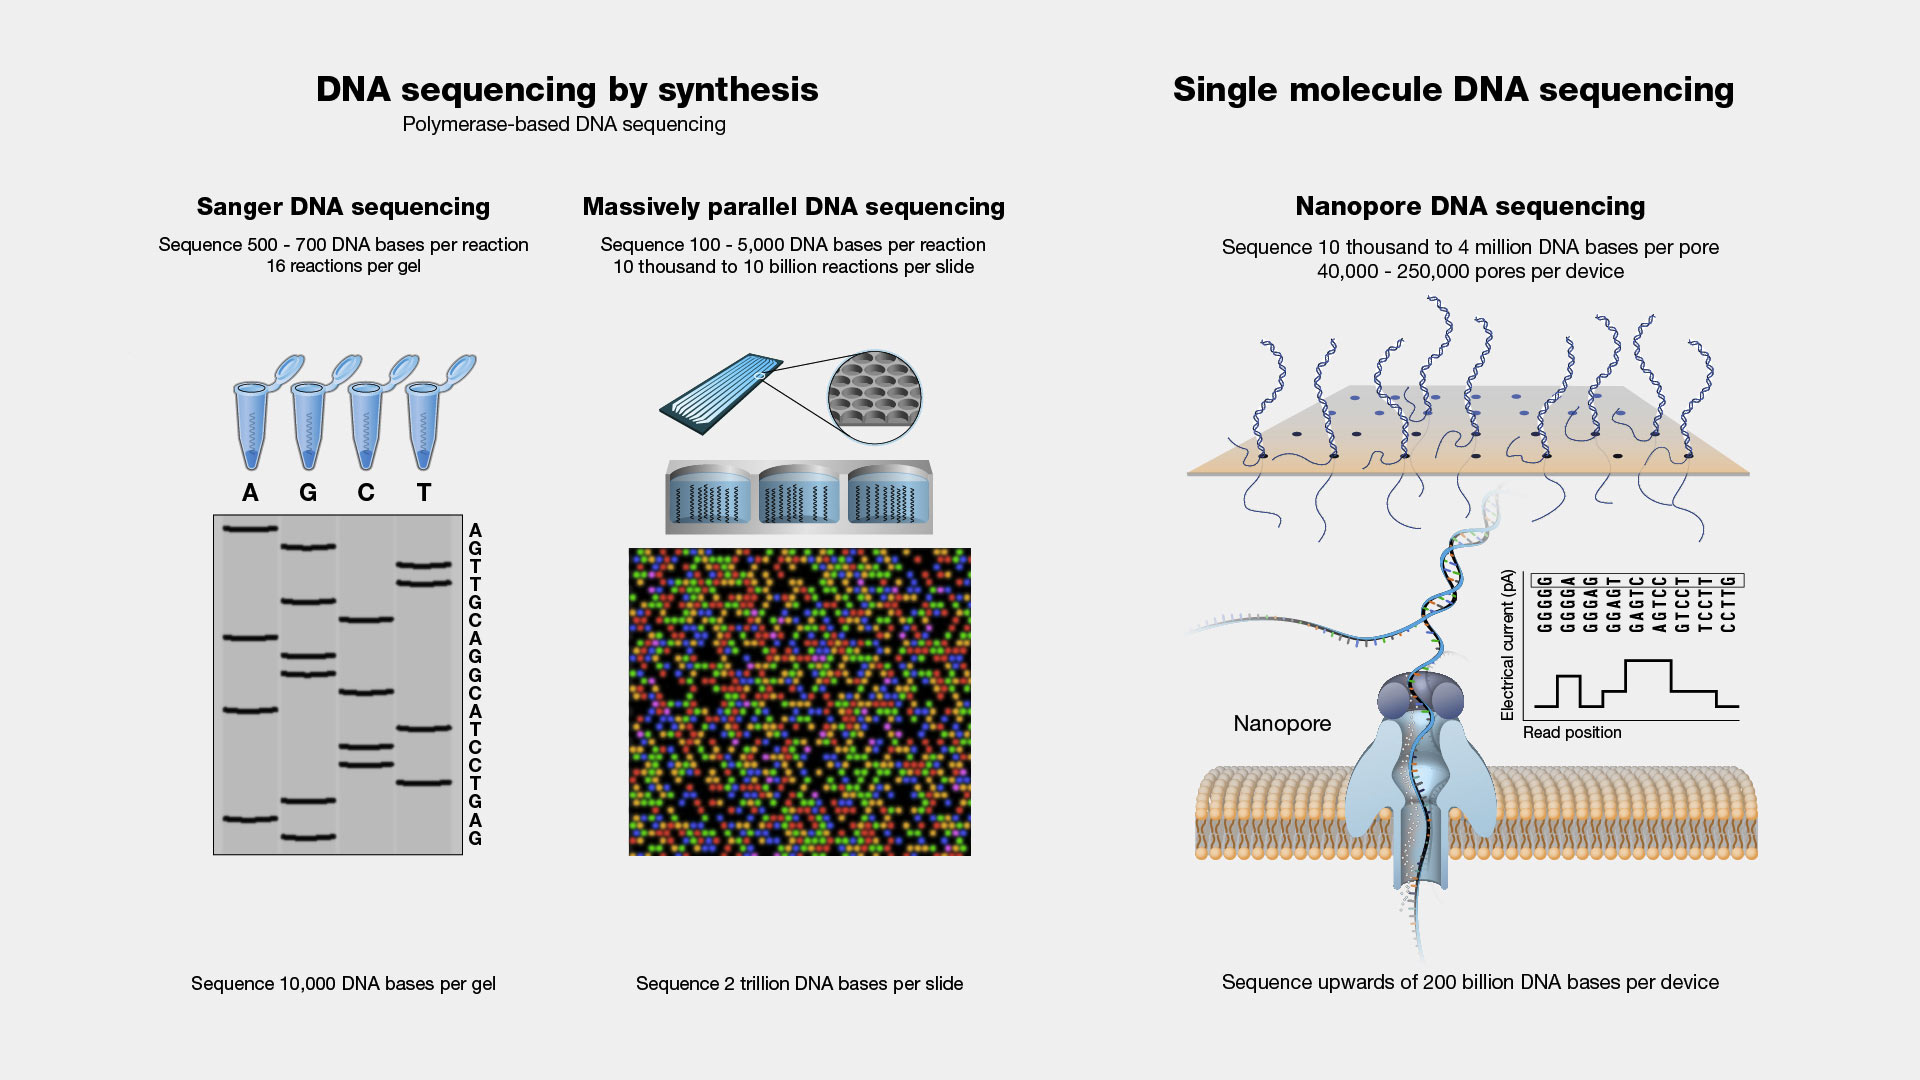
\includegraphics[width=1\linewidth]{images/DNA-Sequencing.jpg}
    \caption[Comparativa tecnologías de secuenciación]{Comparativa tecnologías de secuenciación de ADN\protect\footnotemark.}
    \label{fig:DNA_sequencing}
\end{figure}
\footnotetext{Fuente: https://www.genome.gov/genetics-glossary/DNA-Sequencing}
\subsubsection{Primera generación: Sanger}
Frederick Sanger introdujó la primera generación de tecnologías de secuenciación en el año 1977. El método Sanger utiliza el principio de ``terminación de cadena'' para secuenciar material genético~\cite{sanger1975rapid}. 
%Esta técnica replica el ADN utilizan nucleotidos modificados marcados con fluorescencia que detienen el proceso de replicación.
Durante la PCR se añaden nucleótidos modificados (ddNTPs) marcados con fluoroforo que al ser incorporados en la cadena de ADN detienen la elongación de ésta. Una vez que la reacción ha terminado, se realiza una electroforesis capilar que separa las moleculas de ADN por tamaño y con alta resolución para poder determinar la secuencia de la cadena, generando una única secuencia de como máximo 800 pares de bases por corrida~\cite{crossley2020guidelines}.

La principal ventaja de este método es su alta precisión (99.999\%), siendo ampliamente utilizado en diagnóstico clínico para la detección de mutaciones puntuales. Además de no requerir capacidad de cómputo ni conocimientos bioinformáticos para la generación de la secuencia.  
Entre sus principales desventajas se encuentras que es un método laborioso, costoso e ineficiente al trabajar en proyectos de secuenciación de gran escala como por ejemplo genomas completos o metagenómica debido a la cantidad de información que se puede obtener en la secuenciación, ya que permite obtener una sola secuencia por corrida.
 
Debido a su alta precisión, al secuenciar el gen 16S con Sanger se permite la caracterización a nivel de especie, pero también se pueden encontrar algunas limitantes, como por ejemplo que esta técnica permite detectar una sola especie a la vez. En caso de tener una muestra aislada, la secuenciación permitirá determinar la especie asociada al aíslado, pero en el caso de que la muestra presente más de una bacteria, la señal que se obtendra será una mezcla de las diferentes bacterias, por lo que será imposible realizar una caracterización. 
Esto limita su uso en comunidades complejas o infecciones polibacterianas ~\cite{lamoureux2022prospective}, donde para identificar la comunidad se deben usar tecnologías de secuenciación de nueva generación.
\subsubsection{Segunda generación: Secuenciación de lecturas cortas}
Las tecnologías de secuenciación de segunda generación más importantes son Illumina, IonTorrent y Roche 454. Éstas utilizan el principio de síntesis de cadena complementaria y una señal asociada al nucleótido incorporado (que puede ser fluorescencia, iones cargados, entre otros). %al unirse con la hebra complementaria. 
Esta generación de secuenciadores se caracteriza por ser rápida, de bajo costo, y por permitir obtener simultaneamente millones de moleculas de ADN mediante amplificación clonal o \textit{bridge} PCR, generado en paralelo millones de fragmentos cortos de ADN, de entre 35 a 600 pares de bases, con una precisión de 99.9\%.%, mediante una secuenciación rápida y de bajo costo~\cite{kumar2024next}.


Las principales metodologías de secuenciación de segunda generación son secuenciación por síntesis, utilizada principalmente por Illumina, y secuenciación por ligación utilizada por Roche 454~\cite{mardis2008next}.
Illumina es la \textit{NGS} más utilizada para la secuenciación del gen 16S. Este método utiliza secuenciación por síntesis: la primera etapa corresponde a la fragmentación de ADN y ligación de adaptadores.
Luego los fragmentos de ADN se unen a la superficie de la celda y se amplifican localmente para formar clusters. 
En cada ciclo de secuenciación se añaden nucleótidos marcados con fluoróforos que son removidos para continuar con el siguiente ciclo.
Finalmente, el secuenciador detecta la señal de fluorescencia y registra la secuencia de nucleótidos. 
Illumina posee diferentes dispositivos de secuenciación que permiten obtener \textit{reads} de 2x150 a 2x300 pares de bases como máximo.

Algunas de las plataformas de secuenciación de segunda generación utilizan secuenciación \textit{pair-end} donde cada fragmento de ADN se secuencia en ambas direcciones,  lo que permite obtener fragmentos de mayor tamaño mediante el solapamento de ambas lecturas. 

Dentro de las principales ventajas de las tecnologías de lecturas cortas se encuentra su bajo porcentaje de error, bajo costo, y la gran cantidad de herramientas bioinformáticas ya desarrolladas para trabajar con este tipo de datos~\cite{heather2016sequence}. Por otro lado, el tamaño de los fragmentos secuenciados es su mayor limitante, haciendo más compleja o imposible la resolución de regiones repetitivas o análisis más complejos como el ensamblaje de genomas.


La caracterización de comunidades microbianas con Illumina se ha convertido en el estándar, debido a su bajo costo,througput y alta precisión. Sin embargo las tecnologías de lecturas cortas permiten secuenciar solo una parte del gen 16S rRNA, debido al tamaño de las moleculas que secuencian (lecturas de entre 200 a 400pb)~\cite{salipante2014performance}. 
Diversos estudios se han realizado para analizar qué región permite obtener la mayor diversidad posible y de manera más precisa~\cite{liu2008accurate,schloss2011reducing}. También se ha determinado que existen grupos taxonómicos que se identifican de mejor manera al utilizar cierta regiones hipervariables~\cite{he2013comparison,claesson2010comparison}. De igual forma se ha determinado que al realizar una secuenciación parcial del gen 16S la resolución taxonómica es menor, llegandose a identificar solo hasta el nivel de género~\cite{liu2008accurate}.
 
Es por esto, que las tecnologías de tercera generación, Oxford Nanopore y PacBio se presentan como opciones prometedoras para la secuenciación del gen 16S rRNA, debido a su bajo costo y su capacidad de secuenciar el gen completo en un solo \textit{read}, lo que permite una mayor resolución taxonómica a nivel de especie o incluso de cepa~\cite{szoboszlay2023nanopore,10.1186/s13742}.%~\cite{urban2021freshwater,delahaye2021sequencing}. \hl{revisar estas citas}

%-----------------


%https://sampled.com/short-read-sequencing-vs-long-read-sequencing/#:~:text=Short%2Dread%20sequencing%2C%20as%20the,these%20pieces%20through%20a%20sequencer.

%Al secuenciar el gen 16S con Illumina se sabe que existe presencia de ruido, por lo que se deben realizar filtros como la eliminación de quimeras, eliminación de secuencias singleton y otus raros~\cite{caporaso2011global,auer2017analysis}, realizar denoising con dada~\cite{callahan2016dada2} y unoise~\cite{edgar2016unoise2}. Todas estos filtros y metodologias de trabajo no están disponibles para usarse con TGS como Nanopore y PacBio, debido al porcentaje de error y al tamaño de las lecturas.
%Mientras algunos estudios han demostrado, que Nanopore presenta un porcentaje de ruido muy bajo, casi nulo~\cite{szoboszlay2023nanopore}, y a su vez, al secuenciar el gen completo, y no contar con OTUs, o ASV, permite mejorar el rendimiento de los estimadores de riqueza que se basan en estas metodologias, como los índices de chao1~\cite{chao1984nonparametric}, ACE~\cite{chao1992estimating}, o brakaway~\cite{willis2015estimating}


%Illumina sobrerepresenta el numero de especies debido al ruido? \hl{Nanopore is preferable over ...}


\subsubsection{Tercera generación: Secuenciación de lecturas largas}
Las tecnologías de secuenciación de tercera generación buscan superar las limitaciones de las tecnologías de secuenciación de lecturas cortas, permitiendo obtener información genómica más completa y detallada. % que las tecnologías de secuenciación de segunda generación.
Llegaron a presentarse como una alternativa innovadora y prometedora al poder generar lecturas desde unas pocas kilobases hasta megabases~\cite{amarasinghe2020opportunities}. Junto con su capacidad de secuenciar sin amplificación y en tiempo real. 
Secuenciación de genomas completos, secuenciación de regiones repetitivas, estudios de metilación y bases modificadas son ahora posible de manera más sencilla gracias a la secuenciación de lecturas largas. 
Dentro de esta categoría de plataformas se encuentran Pacific Biosciences (PacBio) y Oxford Nanopore Technologies (ONT).

Mientras PacBio realiza secuenciación por síntesis de moleculas largas, %, donde detectan la incorporación de nucleótidos marcados con fluoróforos en tiempo real mediante el uso de polimerasas\hl{polimerasa XX?}
Oxford Nanopore secuencia mediante la medición de las variaciones de corriente mientras las moleculas de ADN pasan a través de nanoporos, utilizando la diferencia de potencial para determinar la secuencia de nucleótidos.


Su principal ventaja frente a las tecnologías de primera y segunda generación es la obtención de lecturas largas de mas de 1kb, llegando incluso a obtener lecturas de 1.5Mb en el caso de Oxford Nanopore y 200kb en el caso de PacBio, lo que permite la resolución de regiones repetitivas o complejas, como también la identificación de variantes estructurales e identificación de modificaciones epigeneticas de manera mucho más sencilla que al utilizar \textit{short-reads}. 
Dentro de sus principales desventajas se encuentra el porcentaje de error generado por estas plataformas, qué mediante mejoras en la química ha ido disminuyendo pasando de cerca de un 15\% ~\cite{deamer2016three} a menos 1\% para Oxford Nanopore con su nueva química Q20+\footnote{https://nanoporetech.com/accuracy}~\cite{cuber2023comparing} y menor a 0.1\% para PacBio~\cite{cuber2023comparing}.

%Debido a que las tecnologías de tercera generación generan lecturas más largas que las tecnologías de segunda generación, las herramientas utilizadas para caracterizar las comunidades microbianas con las tecnologías cortas son diferentes, ya que no se deben realizar el mismo procesamientos de las secuencias. 
%La cantidad de reads en una posición determinada (ya sea en una referencia o alineadas entre las mismas lecturas) de conoce como \textit{depth} o profundidad, y permite determinar la confianza o precisión de la secuencia~\cite{kumar2024next}.

Con la aparición de las tecnologías de secuenciación de segunda y tercera generación~\cite{janda200716s,pollock2018madness}, la secuenciación del gen 16S rRNA se convirtió en  una técnica masiva para la identificación y caracterización de comunidades microbioanas y de patógenos o aislamiento de bacterias clínicas~\cite{patel200116s}.

%\subsection{xxx}

%El umbral para distinguir especies bacterianas utilizando el gen 16S rRNA es de mínimo 97\% de similitud~\cite{kim2014towards}
%\hl{LEEER} https://www.microbiologyresearch.org/content/journal/ijsem/10.1099/ijs.0.059774-0


%Las tecnologías de secuenciacin de próxima generación presentan ventajas sobre Sanger a la hora de identificación de patogenos, permitiendo la identificacin en pararelo de bacterias en muestras complejas~\cite{peker2019comparison}, como también presenta ventajas tanto en resolución taxonómica como en precisión~\cite{motro2017next}.


%\subsubsection{Aplicación tecnologías de secuenciación para la caracterización de comunidades}



%Ultra-high-throughput microbial community analysis on the Illumina HiSeq and MiSeq platforms.


% \hl{ESTOY VIENDO ACA } https://www.mdpi.com/2076-2607/11/3/804#B1-microorganisms-11-00804
%\subsubsection{Oxford Nanopore}
%\hl{incluso llegandose a secuenciar en el espacio},

%Su bajo costo y su portabilidad, que permiten secuenciar 

%En sus inicios, la mayor limitante de utilizar Oxford Nanopore era su alto porcentaje de error. En el 2019 estudios reportaban que llegar a una resolución de especie no era aún posible con Nanopore~\cite{winand2019targeting}. Estudios posteriores, determinaron que la precisión de secuenciación se encontraba entre el 92\% al cerca del 96\%~\cite{urban2021freshwater,delahaye2021sequencing}, siendo aún inviable para la asignación taxonómica a nivel de especie \hl{creo que deberia tener cuidado con esto, ya que este paper lo dice, pero otros no}. Sin embargo, con la introducción de la nueva química a finales del 2021, el porcentaje de error reportado por nanopore disminuye notablemente, llegando a un 99.9\% de precisión, permitiendo la resolución taxónomica de especie~\cite{yoon2017introducing}.\hl{buscar más citas}


\subsection{Métricas para la evaluación de la diversidad microbiana}
Los índices de diversidad permiten cuantificar y describir propiedades generales de las comunidades, como la riqueza, dominancia, y uniformidad.  %de los diferentes individuos en una comunidad. 
Existen diferentes índices de diversidad, los cuales se pueden dividir en índices de riqueza y de uniformidad, entendiendo la riqueza como el número de especies presentes en una comunidad (sin importar la cantidad de organismos presentes por cada especie) y la uniformidad como la distribución de las abundancias relativas de cada especies.

%Los índices de riqueza permiten evaluar la cantidad de especies presentes en una muestra, mientras que los índices de \hl{uniformidad/divergencia} permiten evaluar la distribución de las especies en la muestra. 
A continuación se presentan algunos de los índices de diversidad más utilizados en la caracterización de comunidades microbianas.   


%dominancia: grado en que uba especie es más abundante que las demás
\subsubsection{Índice de Simpson}
El índice de Simpson mide dominancia y representa la probabilidad de que al seleccionar dos individuos aleatorios de una muestra, ambos pertenezcan a la misma especie. 

Este índice varía entre 0 y 1.  
Valores cercanos a 0 indican una alta diversidad y una baja dominancia de algunas especies en especifico, es decir, al seleccionar dos individuos al azar, la probabilidad de que pertenezcan a la misma especie es baja. 
Valores cercanos a 1 indican una baja diversidad y alta dominancia, es decir una distribución más homogenea. (alta probablidad de que al seleccionar dos individuos al azar sean de la misma especie).
\begin{center}
\begin{math}
D = \sum_{i=1}^{S} \left( \frac{n_i (n_i - 1)}{N (N - 1)} \right)
\end{math}
\end{center}

donde: 
\begin{itemize}
    \item $S$ es el número total de especies
    \item $n_i$ es el número de individuos de la especie $i$
    \item $N$ es el número total de individuos en la muestra
\end{itemize}
Este índice suele expresarse mediante su complemento (1-D) o su inverso (1/D), donde valores cercanos a 1 indican mayor diversidad de especies.

\subsubsection{Índice de Shannon}
Este índice permite cuantificar la variedad de especies, tomando en consideración sus abundancias relativas.

\begin{center}
    \begin{math}
H' = - \sum_{i=1}^{S} p_i \ln(p_i)
\end{math}
\end{center}
donde:
\begin{itemize}
    \item $S$ es el número total de especies
    \item $p_i$ es la proporción de individuos de la especie $i$ respecto al total de individuos
\end{itemize}


Valores mayores a 3 indican una diversidad muy alta, valores entre 2 y 3 indican que las especies estan en equilibrio y valores inferiores a 2 indican baja diversidad.
\subsubsection{Índice de Chao1}
El índice de Chao1 es un estimador de ríqueza que permite obtener un estimado del número total de especies (incluyendo aquellas no detectadas debido a un muestreo insuficiente).
\begin{center}
    \begin{math}
\hat{S}_{Chao1} = S_{obs} + \frac{F_1^2}{2F_2}
\end{math}
\end{center}
donde:
\begin{itemize}
    \item $S_{obs}$ es el número de especies observadas.
    \item $F_1$ es el número de especies observadas que solo se encuentran una vez (singletons).
    \item $F_2$ es el número de especies observadas que se encuentran exactamente dos veces (doubletons).
\end{itemize}
\section{Herramientas}
El desarrollo de un flujo de trabajo automatizado para la caracterización de comunidades microbionas requiere el uso de diferentes herramientas bioinformáticas para el procesamiento de las secuencias, control de calidad, asignación taxonómica con base de datos, análisis de diversidad, caracterización funcional, etc. Por otro lado, el desarrollo de la aplicación web que estará enlazada al flujo de trabajo, requiere del uso diferentes tecnologías web, librerías y de bases de datos para el almacenamiento de la información, generación de gráficos, y procesamiento de información. A continuación se presentan las principales herramientas a utilizar durante esta tesis.
\subsection{Asignación taxónomica}
La asignación taxonómica en el contexto de secuenciación del gen 16S, es el proceso donde dada una secuencia de ADN, se busca identificar a qué organismo pertenece.
Con la secuenciación del gen 16S rRNA se obtiene un conjunto de lecturas (secuencias de nucleótidos), donde cada lectura pertenece a una bacteria presente en la muestra. 
Estas lecturas se procesan y se comparan con bases de datos existentes para poder realizar la asignación taxonómica y poder identificarla. 
Finalmente lo que se obtiene es un perfil de toda la comunidad bacteriana de la muestra, es decir, todas las bacterias presentes que las herramientas bioinformáticas pudieron detectar, junto con su abundancia relativa.


La metodología a utilizar para realizar la asignación va a depender de la tecnología de secuenciación que se haya utilizado.% para Sanger se suele realizar una asignación directa de la lectura que se obtuvo con alguna base de datos como refseq, mientras que para las tecnologías de segunda generación al ser secuencias parciales del gen 16S
Para las tecnologías de tercera generación lo más común es utilizar la base de datos de RefSeq para buscar la secuencia más parecida en la base de datos mediante alguna herramienta de alineamiento como blast.
Algunas metodologías exploran también la corrección de errores de estas secuencias, algoritmos de maximización de expectativas o clustering de las mismas secuencias para aminorizar el porcentaje de error y mejorar la asignación taxonómica. 
%Existen diferentes herramientas para hacer asignación taxonómica de secuencias, algunas incluyen una asignación taxonómica directa a los datos luego del control de calidad, mientras otras herramientas buscan minimizar el error de Oxford Nanopore mediante metodologías de clustering o de algoritmos de maximización de expectativas. 

Algunas de las más utilizadas para trabajar con datos de Oxford Nanopore se presentan a continuación:
%Hoy en día no hay establecidas buenas practicas para el procesamiento del gen 16S rRNA secuenciado mediante Oxford Nanopore, tanto al hablar de la herramienta para hacer asignación taxonómica, como al hablar de la base de datos al utilizar.\hl{leer para ver si citar https://academic.oup.com/femsec/article/97/3/fiab001/6098400}

\subsubsection{Epi2me}
Plataforma desarrollada por Oxford Nanopore para el análisis de datos secuenciación obtenidos mediante sus dispositivos. 
Integra flujos de trabajo para realizar basecalling y demultiplexación, alineamiento, ensamblaje de SARS-CoV-2, asignación taxonómica de gen 16S, 18S, ITS, y metagenómca, variant calling, entre otros.

Mediante la interfaz gráfica el usuario puede seleccionar el análisis a realizar y configurar los parámetros. Debido a su interfaz de fácil uso permite al usuario abstraerse de la ejecución de herramientas o flujos de trabajo y de la necesidad de contar con recursos computacionales para la ejecución de los mismos.
Los resultados se pueden descargar y visualizar mediante la misma plataforma.
%solo requiere acceso a internet por lo que es una buena alternativa para usuarios que no cuentan con recursos computacionales para el analisis de datos de secuenciacion. Sin embargo, la mayoria de sus flujos de trabajo solo cuenta con análisis primarios y no permite la personalización de los scripts o procesos realizados por lo que en caso de requerir una solución personalizada no se podría llevar a cabo mediante la plataforma. De igual manera, al contar solo con analisis primarios, los analisis posteriores deben ser realizados por el usuario mediante el uso de otras herramientas. 


Para la asignación taxónomica del gen 16S utiliza la herramienta blast con la base de datos de Genbank.

% \begin{itemize}
%     \item Qscore mínimo: 7
%     \item Longitud de lectura mínima: 0
%     \item Longitud de lectura máxima: 0
%     \item e-value máximo: 0.01
%     \item coverage mínimo: 30\%
%     \item Porcentaje de identidad mínimo: 77\%
%     \item max target sequences:
% \end{itemize}
Esta herramienta entrega un archivo en formato CSV con la información de la lectura, asignación taxonómica a nivel de especie, porcentaje de identidad de la asignación, entre otras.
\subsubsection{NanoCLUST}
Nanoclust~\cite{10.1093/bioinformatics/btaa900} es un flujo de trabajo desarrollado en Nextflow para la clasificación de amplicones del gen 16s obtenidos mediante secuenciación de Oxford Nanopore. Incluye pasos previos a la asignación taxonomica, como el basecalling, demultiplexación y control de calidad. Destaca por utilizar un clustering no supervisado (UMAP) y un paso exhaustivo de corrección de lecturas basada en los clusters obtenidos previo a la asignación taxonómica.
Utiliza la base de datos de Genbank para realizar la asignación taxonómica.

Cabe destacar que este flujo de trabajo se encuentra descontinuado ya que fue desarrollado utiilzando Nextflow DSL1 (estándar deprecado en la version 22.10). Además, debido a que la herramienta ha dejado de recibir soporte por parte de los desarrolladores, no se han actualizado las versiones de los software ni se han realizado mejoras.

Esta herramienta entrega un archivo csv por cada categoría taxonómica (filo, clase, orden, familia, género, especie) con la cantidad de lecturas asignadas a cada taxonomía. De igual forma, se generan graficos de barra con las asignaciones, y un gráfico de la separación de los clusters. 
\subsubsection{NanoRTax}

NanoRTax~\cite{RODRIGUEZPEREZ20225350} es un flujo de trabajo desarrollado en Nextflow que cuenta con una interfaz web que permite al usuario visualizar el progreso y resultados del pipeline.
Recibe como entrada los archivos FASTQ, a los cuales se les hace un control de calidad mediante fastp, y a continuación se realiza la asignación taxonómica mediante las herramientas Kraken2, Centrifuge y BLAST. 

Al igual que NanoCLUST, NanoRTax utiliza DSL1 por lo que no es comptabile con versiones nuevas de Nextflow.
\subsubsection{EMU}
EMU~\cite{curry2022emu} busca realizar una corrección de errores y mejorar el error de Oxford Nanopore mediante un enfoque basado en algoritmos de maximización de expectativas para generar perfiles taxonómicos de la comunidad microbiona. Permite realizar estos perfiles utilizando diferentes bases de datos, como, la base de datos de Genbank,  RDP y Silva v.138. En el caso de realizar analisis de la región ITS, permite integrar las base de datos de UNITE de fungi y eucariotas.

El output de esta herramienta es un archivo en formato TSV con los perfiles taxonómicos encontrados en cada muestra, es decir, el identificador del taxón, abundancia, especie y la información de todas las categorías taxonómicas. 

% \subsubsection{EzBioCloud Microbial Taxonomic Profiling (MTP) pipeline and the PKSSU4.0 database}
% En algunos estudios se ha utilizado % https://www.mdpi.com/2076-2607/11/3/804#B1-microorganisms-11-00804 , 
% \subsubsection{VSEARCH [35] against the EzBioCloud 16S database.?}


\subsection{Herramientas bioinformáticas}
Existen diferentes herramientas bioinformáticas que se pueden utilizar para el análisis y manipulación de datos de secuenciación, a continuación se presentan algunas de las más relevantes para este trabajo:

% \subsubsection{Guppy}
% Guppy es una suite de herramientas provista por Oxford Nanopore para realizar procesamientos de datos de secuenciación básicos. Permite realizar basecalling y demultiplexación, alineamiento, detección de bases modificadas, etc.
\subsubsection{FastQC}
FastQC\cite{andrews2010fastqc} permite visualizar la calidad de los datos mediante métricas estándar de calidad, contenido GC, distribución de tamaños, niveles de duplicación  y contenido de adaptadores.


Genera un reporte en formato html de fácil visualización separado por módulos, donde cada módulo presenta un estado de Aprobado, Fallido o Advertencia (dependiendo de la calidad de los datos). Se desarrollo pensando en tecnología de secuenciación de lecturas cortas, las cuales poseen un porcentaje de error mucho más bajo (menor al 0.1\%) que las tecnologías de secuenciación de tercera generación y en análisis de genoma completo, por lo que algunos módulos pueden mostrarse como fallidos debido a la naturaleza de los datos de Oxford Nanopore, sin ser datos de baja calidad.
\subsubsection{NanoPlot}
NanoPlot~\cite{10.1093/bioinformatics/btad311} es una herramienta para la evaluación de calidad de datos de secuenciación de lecturas largas, permite visualizar la información de calidad, largo de lecturas y distribución de estas mediantes gráficos interactivos.

Genera un reporte en formato html y gráficos interáctivos que permiten visualizar la calidad de los datos, longitud de las lecturas, distribución de la calidad y longitud, entre otros.
\subsubsection{Fastp}

Fastp\cite{chen2018fastp} es una herramienta de alto rendimiento diseñada para el procesamiento de archivos de secuenciación con calidad (fastq), permite realizar filtrado de secuencias (por calidad, largo), recortar extremos de baja calidad, recortar adaptadores, eliminar colas polyA, etc.
\subsubsection{MultiQC}
MultiQC \cite{ewels2016multiqc} es una herramienta que permite resumir la información obtenida por diferentes herramientas bioinformaticas en un solo informe final. También permite integrar varias muestras en un solo reporte, y multiples pasos de analisis en un solo archivo html.

% Permite una visualización interactiva de los graficos, mediante la cual se puede hacer zoom o quitar muestras de los 

\subsubsection{Seqkit}

\subsubsection{PICRUSt2}
PICRUSt2~\cite{douglas2020picrust2} es una herramienta para la predicción funcional utilizando secuencias marcadoras de genes.
Generalmente se utiliza el gen 16S rRNA para realizar la predicción, pero también se pueden usar otros genes marcadores.

El output entrega archivos en formato CSV con la abundancia de los genes ortologos, la clasificación de las enzimas y las vías metabolicas predichos en cada muestra.

\subsubsection{LEfSe}
LEfSe (Linear discriminant analysis Effect Size)~\cite{segata2011metagenomic}  determina las caracteristicas que permiten explicar las diferencias entre diferentes clases o grupos al combinar pruebas estándar de significancia estadistica junto con pruebas que codifican la consistencia biologica y relevancia del efecto encontrado. 
\subsubsection{vegan package}
Vegan~\cite{dixon2003vegan} es un paquete desarrollado para R que permite realizar análisis de la ecología comunitaria descriptiva. Contiene funciones de análisis de diversidad,  metodos de ordenación comunitaria, análisis de disimilitud, funciones para vegetación y ecologos comunitarios.

% Tiene como objetivo el desarrollo 


\subsubsection{Taxonkit}
Taxonkit~\cite{SHEN2021844} permite la manipulación de información taxónomica de registros de NCBI de una manera eficiente. Dado un identificador taxonómico o un nombre de especie se puede obtener el linage completo de esta.

\subsubsection{csvtk}
csvtk es una herramienta multiplataforma, eficiente y practica para la manipulación de archivos en formato CSV y TSV. Esta herramienta esta desarrollada para utilizarse en conjunto con otras suites de herramientas como TaxonKit, permitiendo obtener resultados de taxonómia de fácil visualización y manipulación para la integración en flujos de trabajo o scripts.
\subsection{Lenguajes de programación y Frameworks}
\subsubsection{Nextflow}
Nextflow~\cite{di2017nextflow} es un framework open source para el desarrollo de flujos de trabajo, el cual permite la ejecución de éstos en diferentes entornos computacionales, ya sea en un computador personal, una plataforma de cómputo de alto rendimiento o en la nube. También permite la ejecución de flujos de trabajo de manera paralela, manejando los recursos computacionales de manera eficiente, y sencilla para el usuario.
 Al permitir el desarrollo de flujos de trabajo escalables y reproducibles es una buena alternativa que ha ganado popularidad debido a su facilidad de uso.

Cuenta con una comunidad llamada nf-core que se encarga de desarrollar flujos de trabajo para el análisis de datos biologicos, los cuales son revisados por la comunidad y publicados en su repositorio. Esto permite contar con una gran cantidad de flujos de trabajo disponibles, los cuales pueden ser ejecutados de manera sencilla por los usuarios, pero cabe destacar que hay que tener conocimientos de linea de comando para poder ejecutarlos.



\subsubsection{FastAPI}
Framework rápido  y ligero para el desarrollo de APIs modernas de manera ágil utilizando Python y basado en sus anotaciones de tipo estandar.
Utiliza pydantic para la validación de los datos de entrada y salida y starlette para el manejo de las peticiones HTTP. %\hl{no estoy 100\% segura}
\subsubsection{SQLalchemy}
Librería de Python que permite la comunicación con base de datos no relacionales de manera sencilla, transformando los registros de la base de datos en objetos utilizables mediante Python. Gestiona la creación de modelos y consultas de forma sencilla.
\subsubsection{Vue.js}
Vue es un framework para la construcción de interfaces de usuario. Se basa en JavaScript, HTML y CSS para proporcionar un modelo de programación declarativo y basado en componentes que permite desarrollar interfaces de manera eficiente.
\subsubsection{TypeScript}  
TypeScript~\cite{bierman2014understanding} es un lenguaje de programación basado en JavaScript, el cual añade sintaxis adicional a JavaScript (o frameworks basados en JS) para soportar la integración de tipado de datos. Al especificar los tipos de datos, TypeScript tiene la capacidad de validarlos e informar errores cuando estos no correspondan.
\subsubsection{Vuetify}
Vuetify es un proyecto de código abierto para la construcción de interfaces utilizando los componentes de Vue. Permite la personalización de los componentes con SASS y SCSS, cuenta con un diseño responsivo, y una gran cantidad de componentes ya predefinidos.
\subsubsection{PostgreSQL}
PostgreSQL es un sistema de gestión de bases de datos relacionales de código abierto que se presentó como la continuación de POSTGRES. Permite el uso de tipos de datos complejos realizar consultas tanto relacionales (SQL) y no relacionales (JSON).

\subsection{Gestores de paquetes}
\subsubsection{Conda}
Conda~\cite{anaconda}  es una herramienta de código abierto, multiplataforma  que permite la gestión de paquetes, dependencias y entornos de desarrollo de manera sencilla. Permite aislar entornos virtuales con caracteristicas especificas, lo que facilita la reproducibilidad de los análisis y la portabilidad de los mismos.
\subsubsection{Apptainer}
Apptainer (antes llamado Singularity~\cite{kurtzer2017singularity}) simplifica la creación y ejecución de contenedores, asegurando el encapsulamiento de los componentes de softwares necesarios para su reproducibilidad y portabilidad.  


\chapter{Flujo de trabajo y Aplicación Web}

\begin{figure}[H]
    \centering
    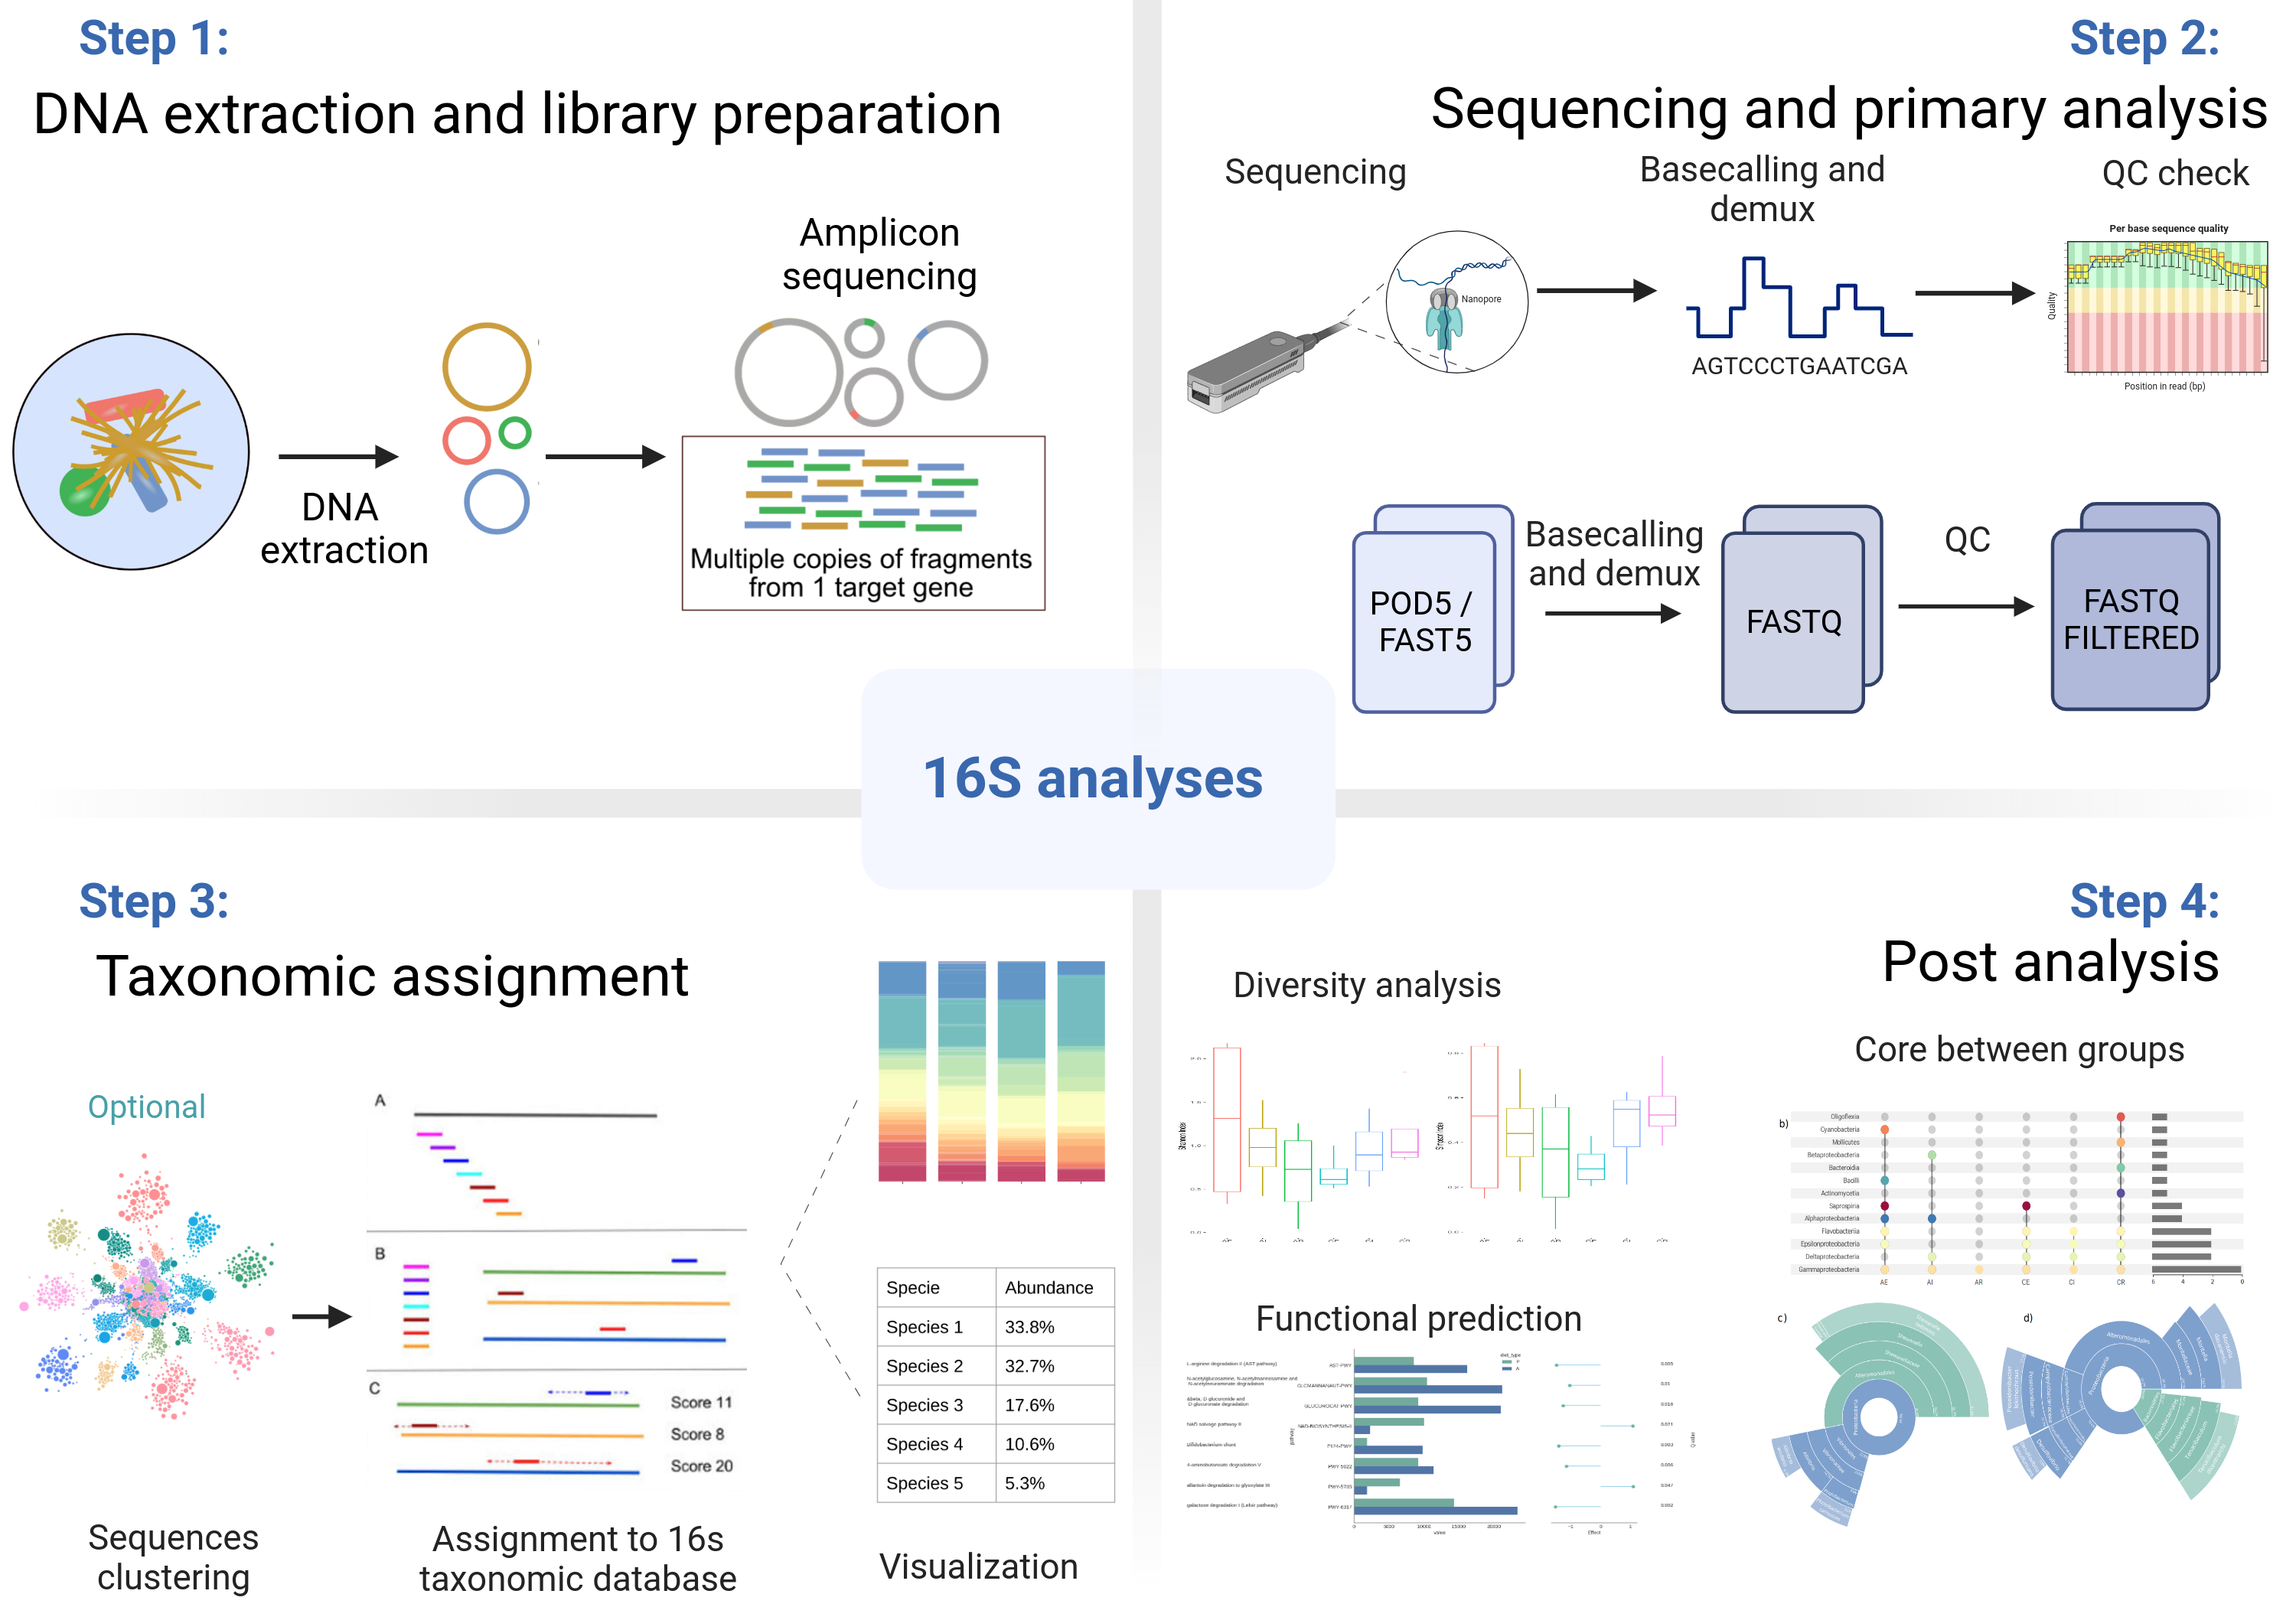
\includegraphics[width=1\linewidth]{images/16s_workflow_schema.jpeg}
    \caption{Flujo de trabajo estándar para la secuenciación y análisis de secuenciaciones del gen 16S}
    \label{fig:16S_workflow}
\end{figure}
\section{Flujo de trabajo}
Se desarrolló un flujo de trabajo automatizado en Nextflow que permite el análisis y la caracterización de secuencias del gen 16S obtenidas mediante dispositivos de secuenciación de Oxford Nanopore. 
El flujo de trabajo está diseñado de manera modular permitiendo que el usuario pueda personalizar su ejecución, agregando o quitando módulos de análisis mediante un archivo de configuración en formato \textit{YAML}.  

El pipeline cuenta con los siguientes módulos: 
\begin{itemize}
    \item Basecalling y demultiplexación (\textit{basecalling}): Este módulo se encarga de realizar el basecalling y demultiplexación de las muestras mediante la herramienta Guppy.
    \item Control de calidad (\textit{qc}): Este módulo se encarga de realizar los filtros y control de calidad de las muestras mediante las herramienta Nanoplot y Fastp.
    \item Asignación taxonómica (\textit{taxonomic\_assignament}): Este módulo se encarga de realizar la asignación taxonómica de las muestras mediante la herramienta BLAST y la base de datos de 16S Genbank. Previo a la asignación taxonómica se realiza un subsampleo de las muestras y se convierten los archivos FASTQ a formato FASTA.
    \item Índices de diversidad (\textit{diversity}): Este módulo se encarga de calcular los índices de diversidad de Shannon, Simpson y Chao1 mediante el paquete vegan de R.
    \item Predicción funcional (\textit{functional\_predicction}): Este módulo se encarga de realizar la predicción funcional de las muestras mediante la herramienta PICRUSt2 y la búsqueda de vías metabólicas que presentan diferencias significativas entre grupos mediante la herramienta Lefse.
\end{itemize}

En los módulos de asignación taxonómica, índices de diversidad y predicción funcional mediante scripts en python se resume la información mediante tablas y se generan gráficos de los resultados obtenidos.

En caso de que el flujo de trabajo se esté ejecutando desde la aplicación web, se ejecutará además un módulo extra que permite escribir los resultados en la base de datos.

\subsection{Archivo de configuración}
El formato YAML se caracteriza por ser un formato de serialización de datos legible por humanos y fácil de interpretar por máquinas.
Tiene una estructura jerárquica que permite la representación de datos de manera más clara y concisa que otros formatos como JSON o XML.

Mediante este archivo de configuración se van a especificar los parámetros necesarios para la ejecución del flujo de trabajo.
Además, el archivo de configuración incluye información sobre los archivos de entrada del flujo de trabajo, nombres de las muestras y grupos asociados, todo en un formato de diccionario.

Para especificar parámetros de un módulo se debe indicar la clave asociada del módulo seguido por \textit{:} y a continuación el nombre del parámetro a modificar y su valor en formato \textit{clave: valor} en la siguiente línea.

Las claves utilizadas en el archivo de configuración para los módulos son las siguientes: \textit{basecalling}, \textit{qc}, \textit{taxonomic\_assignament}, \textit{diversity} y \textit{functional\_prediction}.
A continuación se detallan los parámetros que se pueden modificar en el archivo de configuración y se presenta un ejemplo de archivo de configuración.%(\ref{verb:config}):

\begin{itemize}
    \item \textit{run}: Permite activar o desactivar el módulo. Los valores posibles son ``ON'' o ``OFF''. 
    \item \textit{qc.min\_length}: Permite modificar la longitud mínima requerida de las secuencias. Por defecto es 1000.
    \item \textit{qc.max\_length}: Permite modificar la longitud máxima permitida de las secuencias. Por defecto es 2000.
    \item \textit{qc.min\_qscore}: Permite modificar la calidad mínima requerida de las secuencias. Por defecto es 15 (96,8\% de precisión) .
    \item \textit{qc.subsampling}: Permite modificar la cantidad de lecturas utilizadas para el subsampleo. Por defecto es 100.000.
    \item \textit{qc.save\_reads}: Permite activar o desactivar el guardado de los archivo fastq filtrados en el directorio de resultados. Valores posibles True o False. Por defecto False. 
    \item \textit{taxonomic\_assignament.perc\_identity}: Porcentaje de posiciones idénticas en la secuencia de alineamiento.
    \item \textit{taxonomic\_assignament.evalue}: Valor máximo de evalue aceptado.
    \item \textit{taxonomic\_assignament.qcovs}: Porcentaje de cobertura mínima de alineamientos con altos puntajes.
    \item \textit{taxonomic\_assignament.blast\_db}: Permite ingresar la ruta al directorio que contiene la base de datos de 16S de Genbank (ver sección~\ref{pipeline:how_to_run} para más información).
    \item \textit{group}: Permite ingresar los grupos asociados a las muestras en formato \textit{clave:valor}.
    \item \textit{input}: Permite ingresar el archivo en formato CSV que contiene las columnas samples y fastq.
    \item \textit{outdir}: Permite ingresar el directorio donde se guardaran los resultados del flujo de trabajo.
\end{itemize}

A continuación se presenta un ejemplo de archivo de configuración donde el módulo de basecalling se encuentra desactivado, y los módulos de control de calidad, asignación taxonómica, índices de diversidad y predicción funcional se encuentran activados.
Además se especifican todos los parámetros por defecto del flujo de trabajo, junto con un ejemplo de grupos asociados a las muestras y la ruta al archivo de metadata.



% Además se requiere un archivo de configuración en formato YAML que contenga los parámetros necesarios para la ejecución del pipeline. 
% A continuación se presenta un ejemplo de archivo de configuración:

\begin{verbatim}
  basecalling:
    run: 'OFF'
    save_reads: False
  qc:
    max_length: '2000'
    min_length: '1000'
    min_qscore: '15'
    run: 'ON'
    subsampling: '50000'
    save_reads: False
  taxonomic_assignament:
    run: 'ON'
    blast_db: 'db/'
  diversity:
    run: 'ON'
  functional_prediction:
    run: 'ON'
  group:
    K1.1: Control K
    L1.1: Control L
    L1.2: Control L
    P1.1: No impactadas
    P1.2: No impactadas
    P7.2: Impactadas
    P8.1: Impactadas
  input: samples.csv
  outdir: results
\end{verbatim}
\label{verb:config}

\textit{samples.csv} es un archivo de texto separado por comas (formato CSV) que contiene la información de las muestras a analizar mediante las columnas \textit{samples} y \textit{fastq} \hl{fastq\_2} \hl{group}. 
La columna samples debe contener el nombre con el que se quiere identificar a las muestras y la columna \textit{fastq} la ruta al archivo de secuenciación en formato \textit{fastq}.

\subsection{Estructura del flujo de trabajo}
%El flujo de trabajo se encuentra estructurado por módulos, donde cada módulo se encarga de realizar una tarea específica.

\subsubsection{Basecalling y demultiplexación}
La entrada de este módulo son archivos en formato \textit{POD5} que contienen las secuencias obtenidas en la secuenciación.
El basecalling y demultiplexación se realizan mediante la herramienta Guppy.
%Por defecto se realizará el basecalling de alta preción (HAC).

Para ejecutar este módulo el usuario deben ingresar los siguientes parámetros en el archivo de configuración:
\begin{itemize}
    \item \textit{pod5\_dir}: Directorio que contiene los archivos de secuenciación en formato POD5.
    \item \textit{guppy\_basecalling\_config}: Archivo de configuración a utilizar para hacer el basecalling.
    \item \textit{guppy\_barcoding\_kits}: Kit de barcoding a utilizar para hacer la demultiplexación.
    \item \textit{save\_reads}: Permite activar o desactivar el guardado de los archivos demultiplexados. Valores posibles True o False. Por defecto False.
\end{itemize} 

Por defecto este módulo entrega un archivo HTML con el reporte de la demultiplexación y el basecalling de las muestras (generado con MultiQC), el cual se almacena en la carpeta QC/multiqc\_guppy.html.
En caso de que el usuario quiera almacenar los archivos demultiplexados, debe activar la opción \textit{basecalling.save\_reads} en el archivo de configuración.


\subsubsection{Control de calidad}
Este módulo siempre se ejecuta y es el encargado de realizar los filtros y control de calidad de las muestras.
La entrada de este módulo son archivos en formato \textit{Fastq}, que pueden ser provenientes del módulo anterior (\textit{basecalling y demultiplexación}) o pueden ser indicados por el usuario a través del archivo de configuración.
El control de calidad se realiza mediante la herramienta NanoPlot (antes y después de los filtros).
Los filtros de calidad son llevados a cabo con la herramienta Fastp, utilizando los siguientes parámetros:
\begin{itemize}
    \item calidad mínima: por defecto 15 o valor ingresado en el archivo de configuración \textit{qc.min\_qscore} (\textit{-q 15})
    \item \textit{--cut\_mean\_quality 15}: Permite eliminar bases de baja calidad en los extremos de la secuencia, por defecto 15 (uso en conjunto con \textit{--cut\_front}, \textit{--cut\_tail})
    \item longitud mínima requerida: por defecto 1000 o valor ingresado en el archivo de configuración \textit{qc.min\_length} (\textit{--length\_required 1000}) 
    \item longitud máxima permitida: por defecto 2000 o valor ingresado en el archivo de configuración \textit{qc.max\_length} (\textit{--length\_limit 2000})
    \item deshabilitar la eliminación de adaptadores (\textit{--disable\_adapter\_trimming}) (no modificable)
    \item deshabilitar la eliminación de colas poly g (\textit{--disable\_trim\_poly\_g}) (no modificable)
\end{itemize}

Además, este módulo cuenta con un script desarrollado en Python que permite graficar la longitud promedio versus la calidad promedio de las muestras después de los filtros.

El output de este módulo es una carpeta llamada \textit{QC} que contiene los siguientes directorios:
\begin{itemize}
    \item \textit{fastq\_filtered}: Directorio con archivos FASTQ de las secuencias filtradas (obtenidas con fastp).
    \item \textit{fastp\_reports}: Directorio con los reportes de los filtros de calidad en formato JSON y HTML (obtenidos con fastp).
    \item \textit{nanoplot\_reports/raw|filtered}: Directorio con los reportes de control de calidad de las muestras antes y después de los filtros (obtenidos con NanoPlot).
    \item \hl{multiqc}: Reporte en formato HTML con el resumen de los reportes de NanoPlot y Fastp para los archivos antes y después de los filtros de calidad.
    \item \textit{quality\_plot.pdf}: Gráfico de la longitud promedio versus la calidad promedio de las muestras después de los filtros en una ventana de las posiciones de 1400 a 1600 pares de bases.
\end{itemize}

A continuación se presenta un ejemplo del gráfico de calidad y longitud promedio de las muestras generado por el pipeline (Figura~\ref{fig:pipeline-quality-plot}).
\begin{figure}[H]
    \centering
    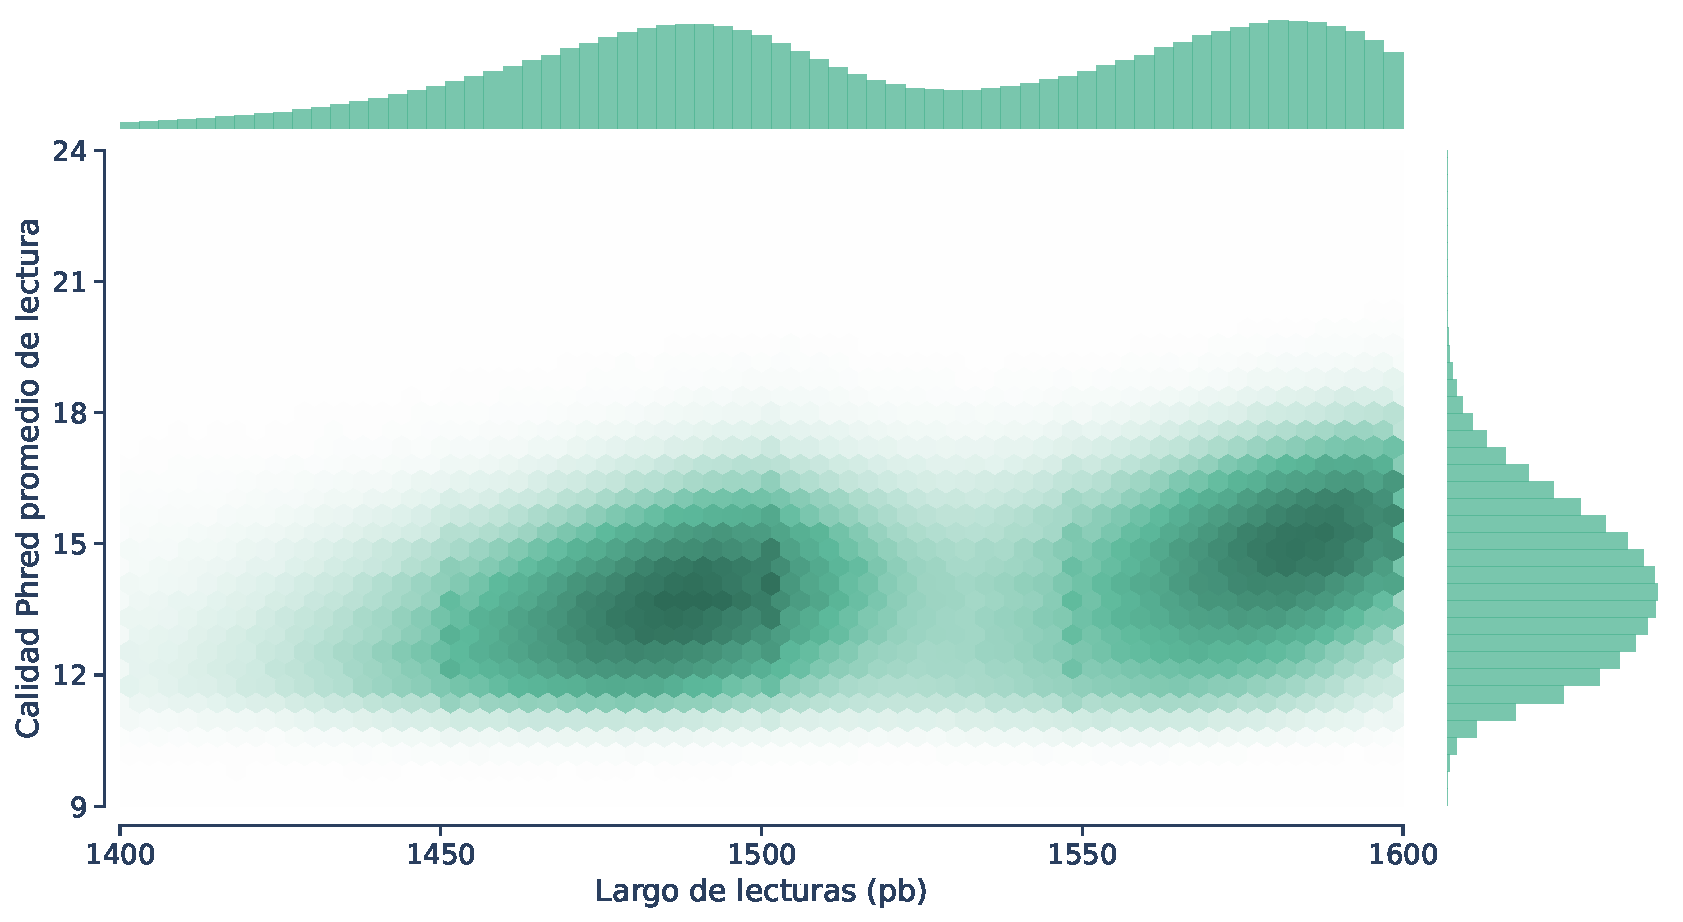
\includegraphics[width=0.85\linewidth]{images/pipeline/quality_plot.pdf}
    \caption{Gráfico de calidad vs longitud promedio. En el eje X esta la longitud de las lecturas, mientras en el eje Y se encuentra la calidad promedio.}
    \label{fig:pipeline-quality-plot}
\end{figure}
\subsubsection{Asignación taxonómica}
Este módulo se ejecuta siempre que el parámetro de asignación taxonómica sea ``ON'' en el archivo de configuración. 
La ruta a la base de datos debe ser especificada mediante el parámetro \textit{taxonomic\_assignament.blast\_db}.
La entrada de este módulo son archivos en formato \textit{FASTQ} que provienen del módulo anterior (\textit{control de calidad}).

Previo a la asignación taxonómica, se realiza un subsampleo de las muestras con la herramienta SeqKit para evitar sesgos en la caracterización de la comunidad microbiana debido a alguna desproporción en la cantidad de lecturas de las muestras.
La cantidad de lecturas utilizadas para el subsampling por defecto es 100.000 o el valor ingresado por el usuario en el archivo de configuración \textit{qc.subsampling}.
Posterior a ello se convierten los archivos FASTQ a formato FASTA mediante la herramienta SeqKit.

La asignación taxonómica se realiza mediante la herramienta BLAST (algoritmo blastn) con la base de datos de 16S de Genbank. 
\hl{Para aceptar un match con la base de datos se requiere un valor de identidad mayor al 97\%, una cobertura mayor al 85\% y un evalue menor a 1e-6.}
\hl{Se eliminan todas las taxas con menos de 0.01\% de abundancia.}

Posterior a la asignación taxonómica, mediante la herramienta TaxonKit se obtiene el linaje completo de todas las especies asignadas con BLAST, este resultado se formatea mediante la herramienta CSVTk. 
Esto se realiza con el objetivo de poder graficar todas las categorías taxonómicas tanto en los gráficos de barras apiladas como en el gráfico circular jerárquico.

Mediante un script en python se realiza un resumen de la asignación taxonómica obtenida con BLAST de todas las muestras y los linajes asociados a cada especie en un solo archivo. Además, se generan archivos por cantidad de lecturas y porcentaje, por cada categoría taxonómica y por muestra y grupo (en caso de ingresarse en el archivo de configuración).
Estos archivos son utilizados como entradas para los scripts que generan los gráficos de barras apiladas y  el gráfico circular jerárquico.


En el caso del gráfico circular, se buscan todas las taxonomías compartidas entre las muestras que tengan una abundance mayor al 1\% en al menos una muestra. 
Una vez que se identifican, se suman las lecturas asignadas a cada taxonomía en todas las muestra del grupo y se grafica el porcentaje de lecturas asignadas a cada taxonomía en todas las muestras del grupo como un valor único.



El output de este módulo es una carpeta llamada \textit{taxonomic\_assignament} que contiene los siguientes directorios:
\begin{itemize}
\item \hl{blast\_out}
\item plots: Este directorio contiene los siguientes directorios:
\begin{itemize}
    \item taxonomy\_plots: Directorio con los gráficos de barras apiladas de las taxonomías. Contiene cuatro tipos de gráficos: 
    \begin{itemize}
        \item barras apiladas por muestra utilizando el valor porcentual.
        \item barras apiladas por muestra utilizando la cantidad de lecturas.
        \item barras apiladas por grupos utilizando el valor porcentual.
        \item barras apiladas por grupos utilizando la cantidad de lecturas.
    \end{itemize}
    \item core\_plot: Directorio con los gráficos circulares jerárquicos de las taxonomías compartidas entre las muestras. Habrá un gráfico general que busca las similitudes en todas las muestras, y un gráfico por cada grupo ingresado (en caso de ingresar grupos)(Figura~\ref{fig:pipeline-core}).
\end{itemize}
 \end{itemize}
A continuación se presentan ejemplos de los gráficos generados en este módulo. La figura~\ref{fig:pipeline-stacked-sample} presenta un gráfico de barras apiladas por muestra utilizando el valor porcentual y la categoría de clase, mientras que la figura~\ref{fig:pipeline-stacked-group} muestra un gráfico de barras apiladas por grupos utilizando el valor porcentual.
\begin{figure}[H]
    \centering
    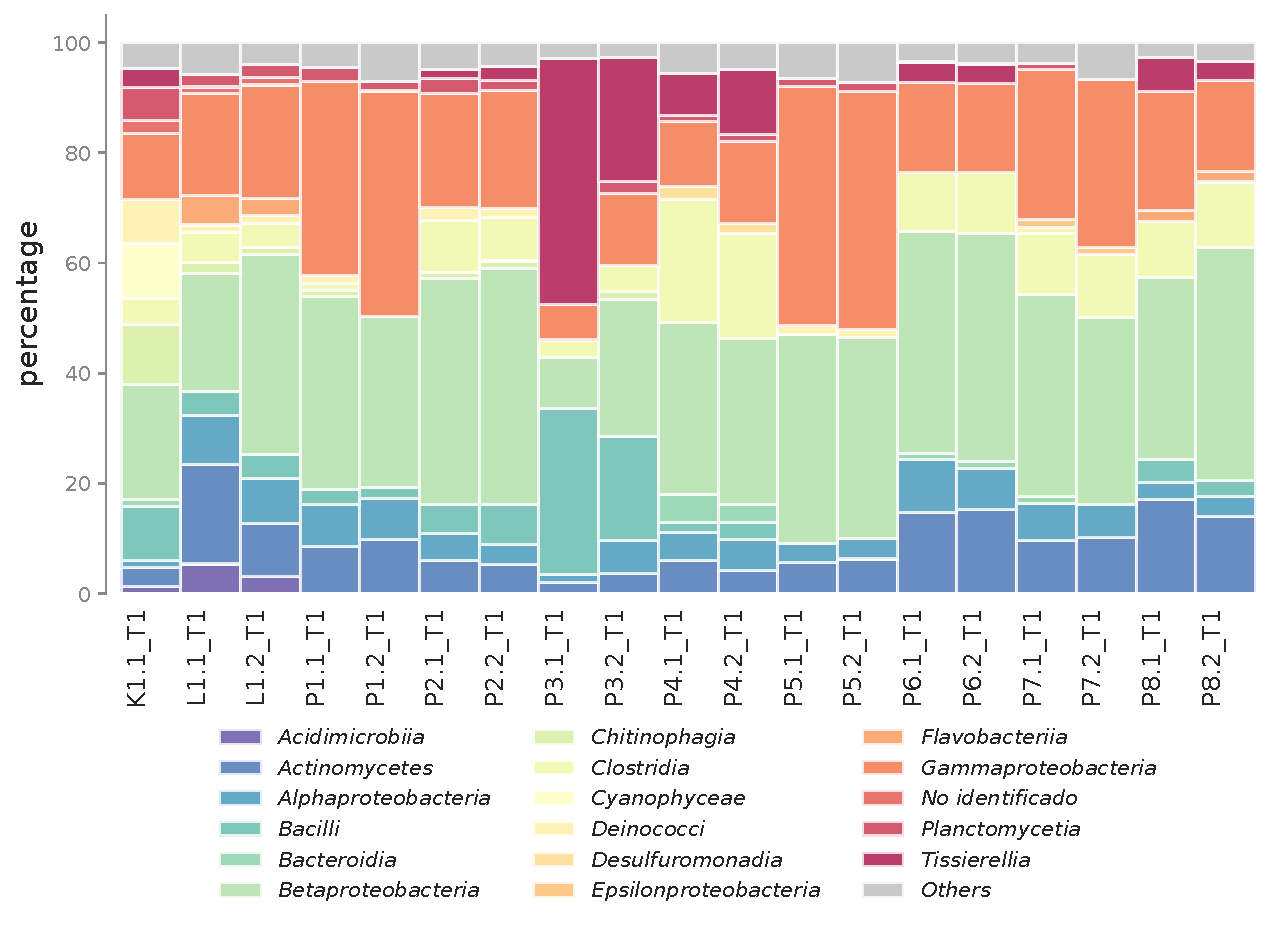
\includegraphics[width=1\linewidth,height=0.4\textheight]{images/pipeline/class_samples_percentage.pdf}
    \caption{Gráfico de barras apiladas por muestra utilizando el valor porcentual y la categoría de clase}
    \label{fig:pipeline-stacked-sample}
\end{figure}
\begin{figure}[H]
    \centering
    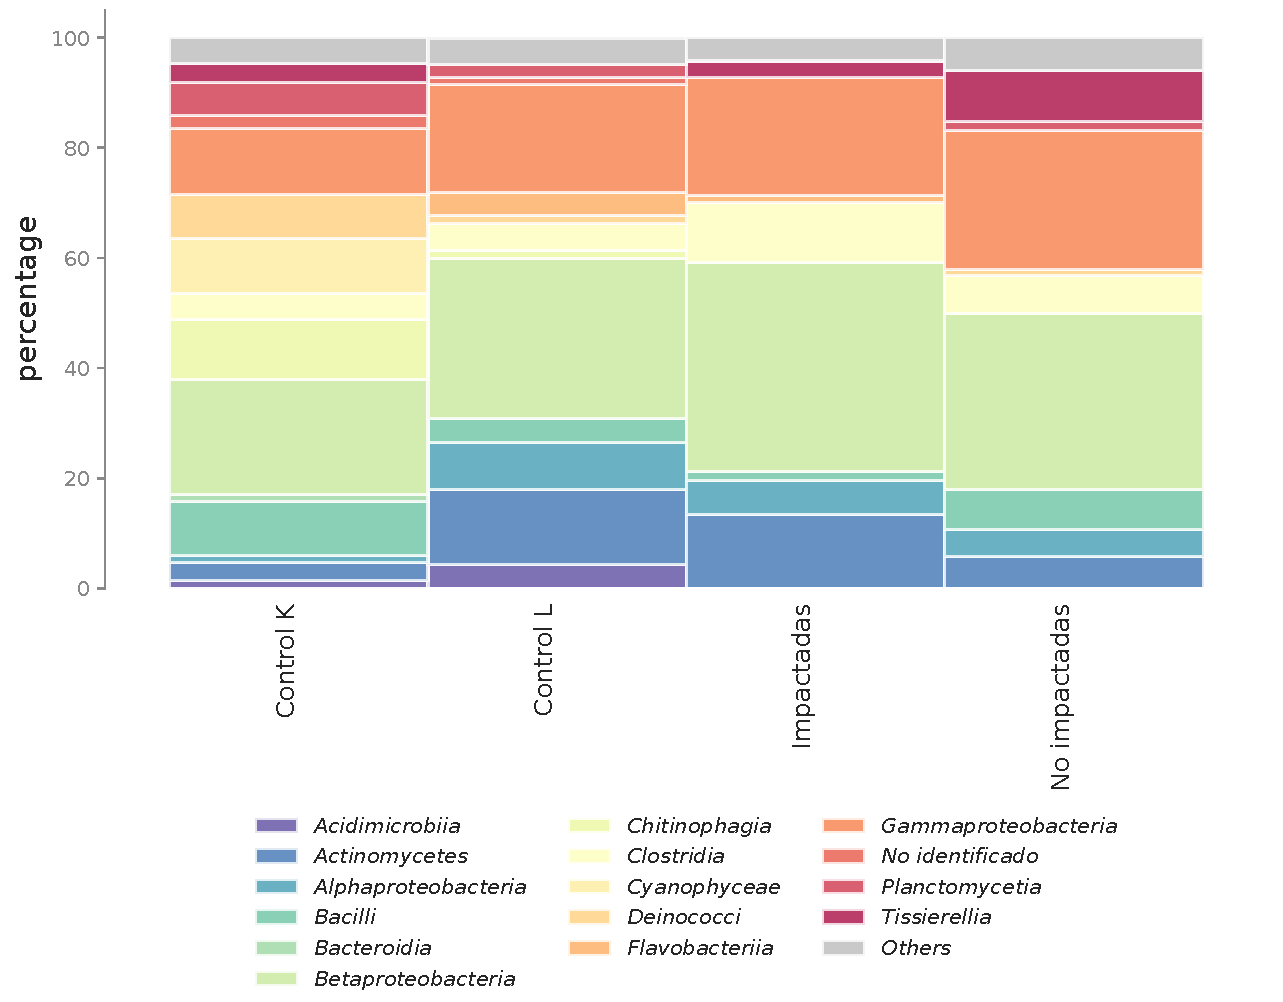
\includegraphics[width=1\linewidth,height=0.4\textheight]{images/pipeline/class_grouped_percentage.pdf}
    \caption{Gráfico de barras apiladas por grupos utilizando el valor porcentual y la categoría de clase}
    \label{fig:pipeline-stacked-group}
\end{figure}

La figura~\ref{fig:pipeline-core} presenta un gráfico circular jerárquico generado para el grupo de muestras categorizadas como No impactadas.
Este gráfico muestra todas las taxonomías compartidas entre las muestras del grupo No impactadas.
\begin{figure}[H]
    \centering
    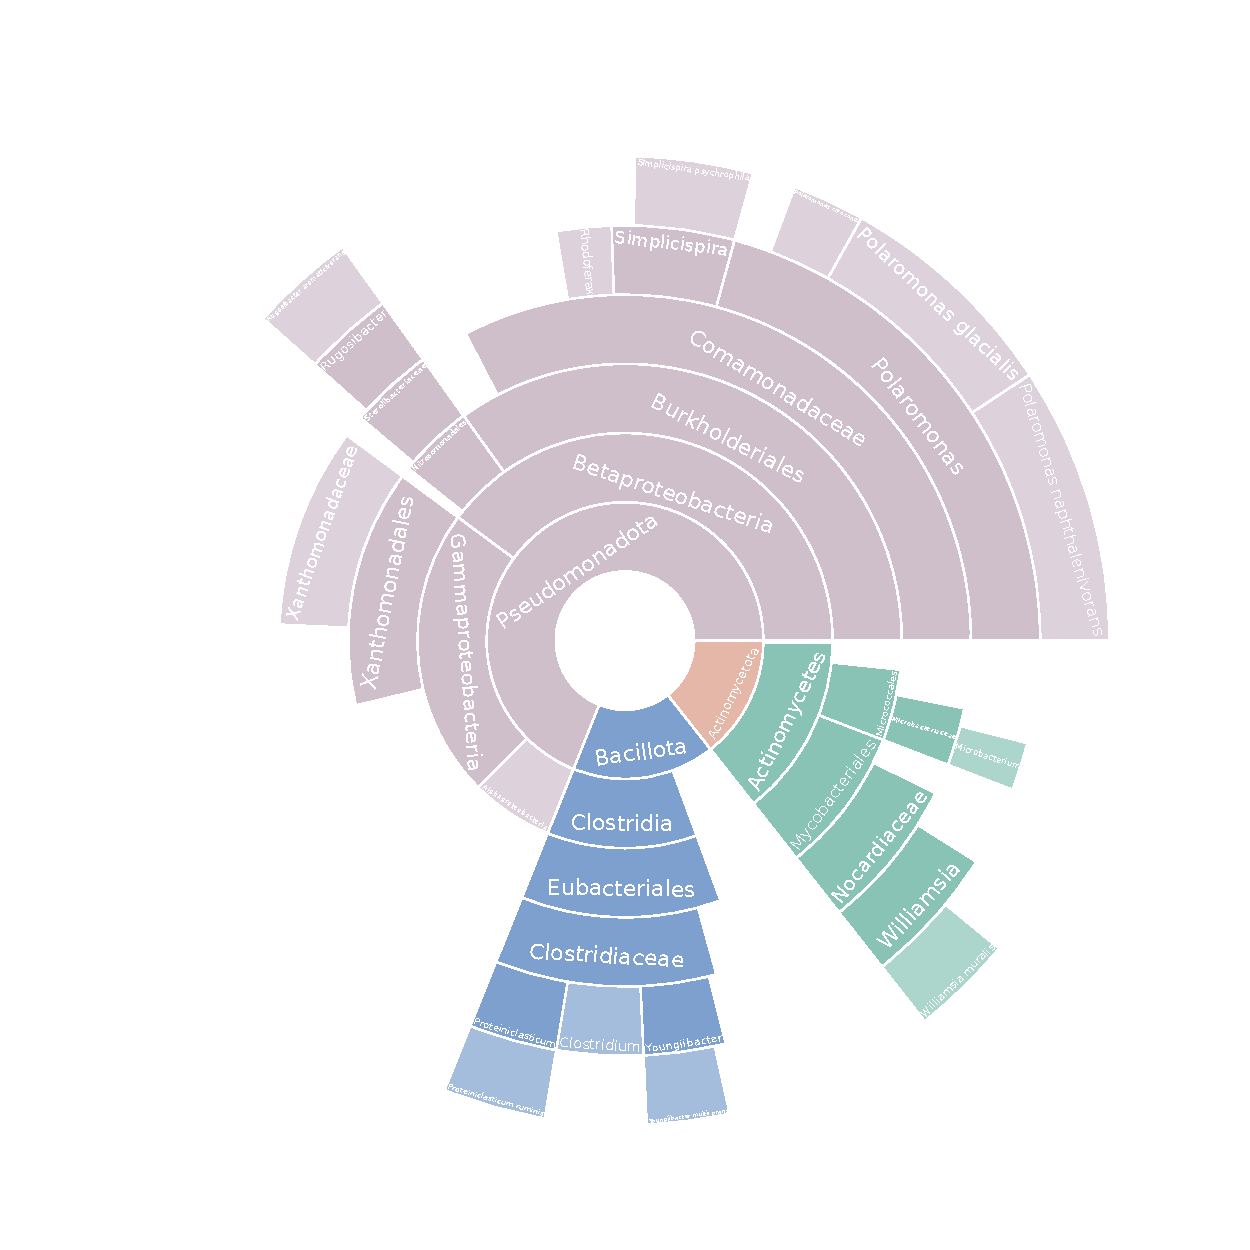
\includegraphics[width=0.9\linewidth]{images/pipeline/core_Impactadas.pdf}
    \caption{Gráfico jerárquico generado para el grupo de muestras categorizadas como No impactadas}
    \label{fig:pipeline-core}
\end{figure}

\subsubsection{Indices de diversidad}
Este módulo solo se ejecutara si el parámetro \textit{diversity.run} es ``ON'' en el archivo de configuración. 
Para poder ejecutarlo se requiere que el usuario haya ingresado grupos asociados a las muestras en el archivo de metadata.

El cálculo de los índices de diversidad se realizará utilizando el paquete \textit{vegan} de R.
La entrada de este módulo es el archivo resumen de blastn obtenido en el módulo anterior (\textit{merge\_blast\_out}) que contiene en las columnas las muestras y en las filas las especies, y  en la intersección la cantidad de lecturas asociadas.
Además del archivo resumen de blast, este módulo requiere los grupos asociados a las muestras en formato diccionario (proveniente del archivo de configuración).

Mediante la función \textit{diversity} se calculan los índices de Simpson y Shannon, y mediante la función \textit{estimateR} se calcula el índice de Chao1.
Utilizando la librería ggplot se representa la información de los índices de diversidad en un gráfico de cajas y bigotes.
Para el cálculo de los índices solo se considerarán aquellos grupos con al menos 3 muestras.

El output de este módulo es una carpeta llamada \textit{diversity} que contiene un archivo csv con los valores de los índices de diversidad calculados para cada muestra y grupo ingresado (\textit{diversity\_index.csv}), junto con el gráfico de cajas y bigotes generado \textit{diversity\_boxplot.pdf}

A continuación se presenta un ejemplo del gráfico de cajas y bigotes generado por el pipeline (Figura~\ref{fig:pipeline-diversity_boxplot}).
\begin{figure}[H]
    \centering
    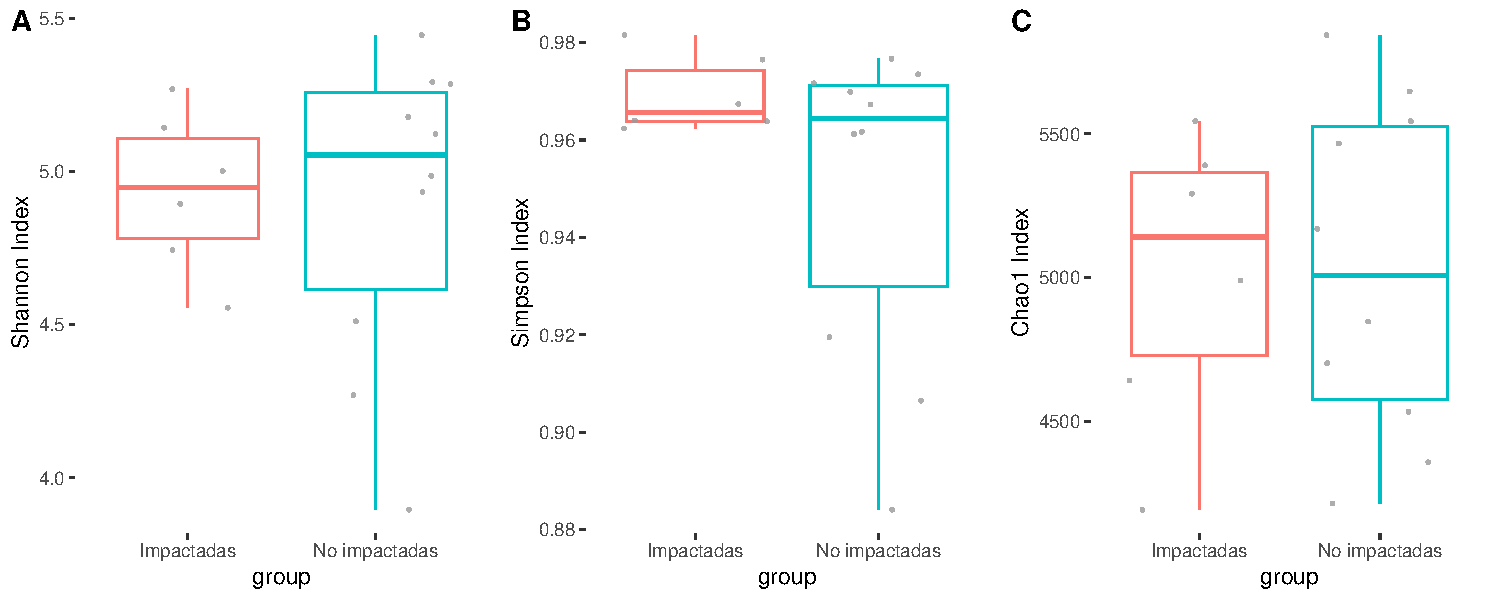
\includegraphics[width=0.9\linewidth]{images/pipeline/diversity_boxplot.pdf}
    \caption{Gráfico de cajas y bigotes de los índices de diversidad calculados para cada grupo ingresado}
    \label{fig:pipeline-diversity_boxplot}
\end{figure}

\subsubsection{Predicción funcional}
Este módulo solo se ejecutará si el parámetro \textit{functional\_prediction.run} es ``ON'' en el archivo de configuración. 
Para poder ejecutar la diferenciación entre grupos se requiere que el usuario haya ingresado esta información en el archivo de metadata.

La predicción funcional se realizará mediante la herramienta PICRUSt2. 
Para disminuir los tiempos de ejecución, se realizará la predicción por muestra y luego mediante un script en python se unirán los resultados en un solo archivo.
Para la búsqueda de vías metabólicas que presentan diferencias significativas entre grupos se utilizará la herramienta Lefse (\hl{valor de normalización}).

El output de este módulo es una carpeta llamada \textit{functional\_prediction} que contiene los siguientes directorios:
\begin{itemize}
    \item \textit{picrust2\_out}: Directorio con los resultados de la predicción funcional por muestra. Contiene los siguientes directorios:
    \begin{itemize}
        \item \textit{EC\_metagenome\_out}: Directorio con los resultados de la predicción de las enzimas EC.
        \item \textit{KO\_metagenome\_out}: Directorio con los resultados de la predicción de los genes KO.
        \item \textit{Pathways\_out}: Directorio con los resultados de la predicción de las vías metabólicas.
    \end{itemize}
    \item \textit{KO.csv}: Archivo resumen con los resultados de la predicción de los genes KO para todas las muestras.
    \item \textit{EC.csv}: Archivo resumen con los resultados de la predicción de las enzimas EC para todas las muestras.
    \item \textit{Pathways.csv}: Archivo resumen con los resultados de la predicción de las vías metabólicas para todas las muestras.
    \item Gráfico de barras con vías metabólicas que presentan diferencias significativas entre grupos
    \end{itemize}

A continuación se presenta el gráfico generado donde se presentan las vías metabólicas que presentan diferencias (obtenidas mediante la herramienta LefSE) significativas entre los dos grupos ingresados  (Figura~\ref{fig:pipeline-lefse}).
    \begin{figure}[H]
        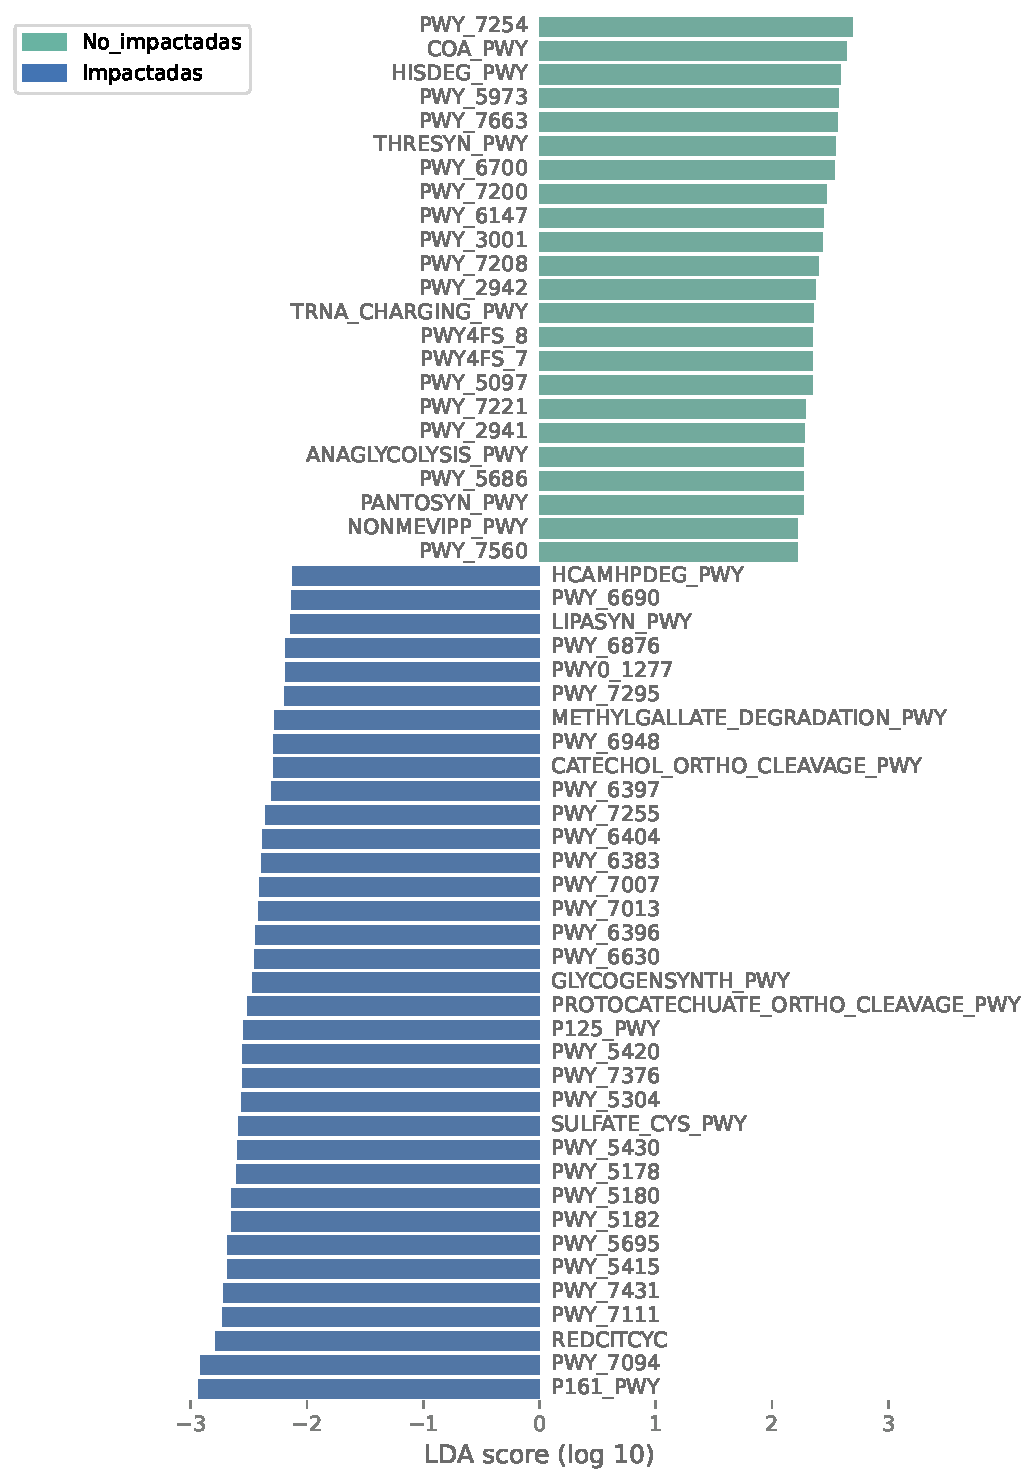
\includegraphics[width=0.7\linewidth]{images/pipeline/lefse_plot.pdf}
        \caption{Barra de navegación}
        \label{fig:pipeline-lefse}
    \end{figure}
\subsubsection{Ejecución del flujo de trabajo}\label{pipeline:how_to_run}
Para ejecutar el flujo de trabajo se debe descargar el ejecutable de Nextflow desde su página oficial\footnote{https://www.nextflow.io/}. 
Además se requiere tener instalado conda para gestionar la instalación de paquetes y herramientas.

Para ejecutar el flujo de trabajo se debe ingresar el siguiente comando en la terminal:
\begin{verbatim}
    nextflow run nanotax-pipeline -profile conda -params-file params.yml

\end{verbatim}
La descarga de la base de datos de 16S de Genbank se puede realizar mediante el FTP de NCBI\footnote{ftp://ftp.ncbi.nlm.nih.gov/blast/db/16S\_ribosomal\_RNA.tar.gz}.

Se recomienda usar la opción \textit{-resume} para reanudar la ejecución en caso de que se haya interrumpido.

\hl{Desarrollo de contenedores o conda enviroments}
Para la reproducibilidad del flujo de trabajo se cuenta con dos \hl{executers}: Conda y \hl{Singularity}    .

\subsubsection{Tiempos de ejecución y requerimientos computacionales}

\newpage
\section{Aplicación Web}
Se desarrollo una aplicación web mediante Vue3, FastAPI y PostgreSQL que permite al usuario subir sus archivos de secuenciación y metadata. 
Con esto el usuario puede abstraerse de tener conocimiento en línea de comando o ejecución de heramientas bioinformaticas y/o flujos de trabajo, 
ya que mediante la interfaz web el usuario solo debe seleccionar los análisis que desea realizar.
La información ingresada por el usuario es guardada en la base de datos y mediante un script se generan los parámetros necesarios para la ejecución del flujo de trabajo.
Una vez el pipeline termina de ejecutarse se escriben los resultados en la base de datos. 
La plataforma lee esta información directa de la base de datos y despliega los resultados en forma de tablas y gráficos en la sección de análisis.


A continuación se detalla cada una de las vistas de la aplicación web y su funcionalidad.
% \subsection{Middleware}
% \subsection{Security}

\subsection{Login}
Al ingresar en la página de Login, el usuario deberá ingresar su nombre de usuario y contraseña.
En caso de que los datos sean correctos será redireccionado a la página de proyectos (Ver sección \ref{projects}).
En caso de que los datos sean incorrectos se mostrará un mensaje de error \textit{“Usuario o contraseña incorrectos”} y deberá ingresar sus credenciales nuevamente.


\begin{figure}[ht]
    \centering
    \begin{subfigure}[b]{0.45\textwidth}
        \centering
        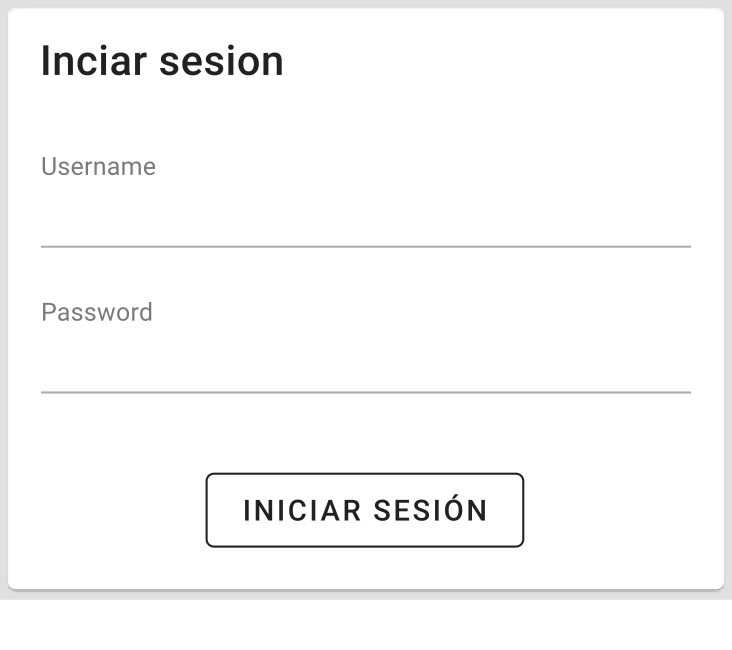
\includegraphics[width=\textwidth]{images/app/login.png}
        \caption{Vista de inicio de sesión por defecto \newline}
        \label{fig:app-login_default}
    \end{subfigure}
    \hfill
    \begin{subfigure}[b]{0.45\textwidth}
        \centering
        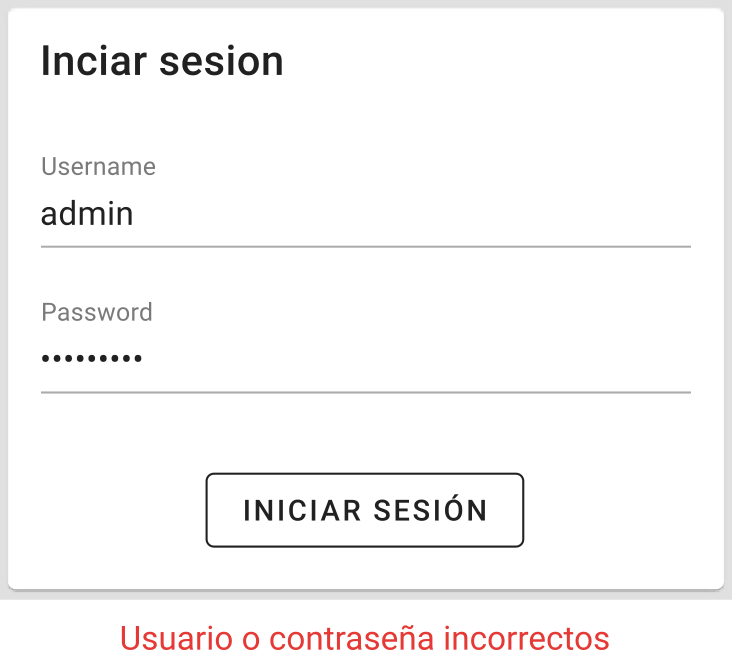
\includegraphics[width=\textwidth]{images/app/login-error.png}
        \caption{Vista de inicio de sesión con mensaje de error al ingresar credenciales inválidas}
        \label{fig:app-login_error}
    \end{subfigure}
    \caption{Vista de Inicio de sesión}
    \label{fig:app-login}
\end{figure}

\hl{Registrarse - vista}
\subsection{Navbar}
Una vez que el usuario inicia sesión, va a poder visualizar la barra de navegación de la plataforma en la parte superior de la página. 
% La plataforma cuenta con las siguientes secciones en la barra de navegación:
% \begin{itemize}
%     \item \textit{Results}
%     \item \textit{New analyses}
%     \item \textit{Change password}: Cambiar contraseña
%     \item \textit{Log out}: Cerrar sesión en la plataforma
% \end{itemize}
\begin{figure}[H]
    
\includegraphics[width=1\linewidth]{images/app/navbar.png}
    \caption{Barra de navegación}
    \label{fig:app-nabvar}
\end{figure}

A continuación se describen las funcionalidades de cada una de las secciones de la barra de navegación:

\subsection{Cambio de contraseña}
Una vez que el usuario validó sus credenciales va a poder acceder a la vista de cambio de contraseña a través de la barra de navegación (Figura~\ref{fig:app-change-psw_default}).



Para realizar el cambio de contraseña, deberá ingresar su contraseña actual y su nueva contraseña dos veces.
En caso de que la contraseña sea cambiada con éxito se mostrará el mensaje \textit{“Contraseña cambiada con exito“} (Figura~\ref{fig:app-change-psw-success}).


\begin{figure}[H]
    \centering
    \begin{subfigure}[b]{0.45\textwidth}
        \centering
        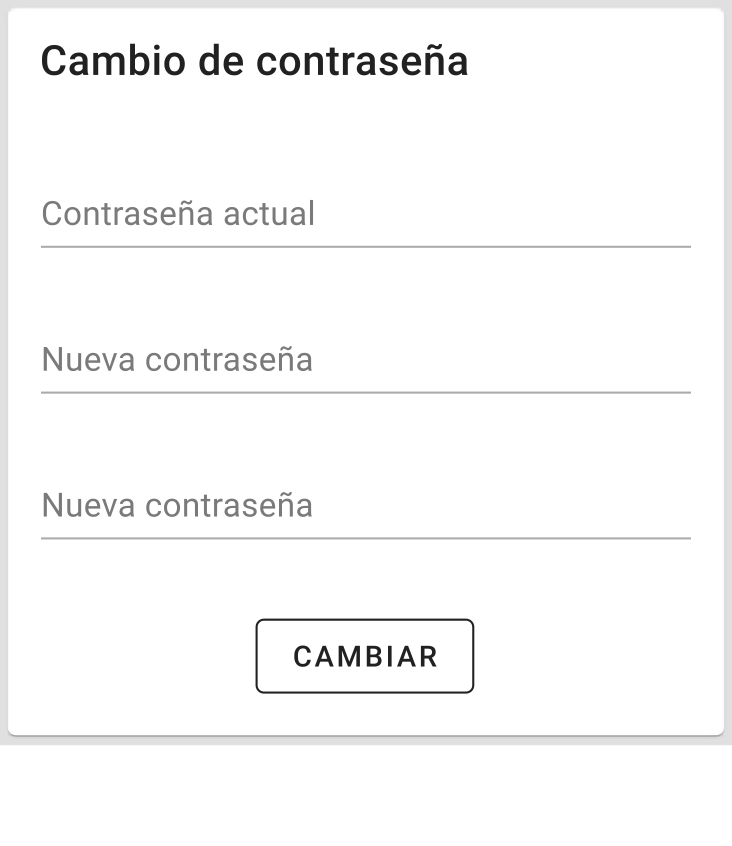
\includegraphics[width=\textwidth]{images/app/change-psw-def.png}
        \caption{Vista de cambio de contraseña por defecto \newline}
        \label{fig:app-change-psw_default}
    \end{subfigure}
    \hfill
    \begin{subfigure}[b]{0.45\textwidth}
        \centering
        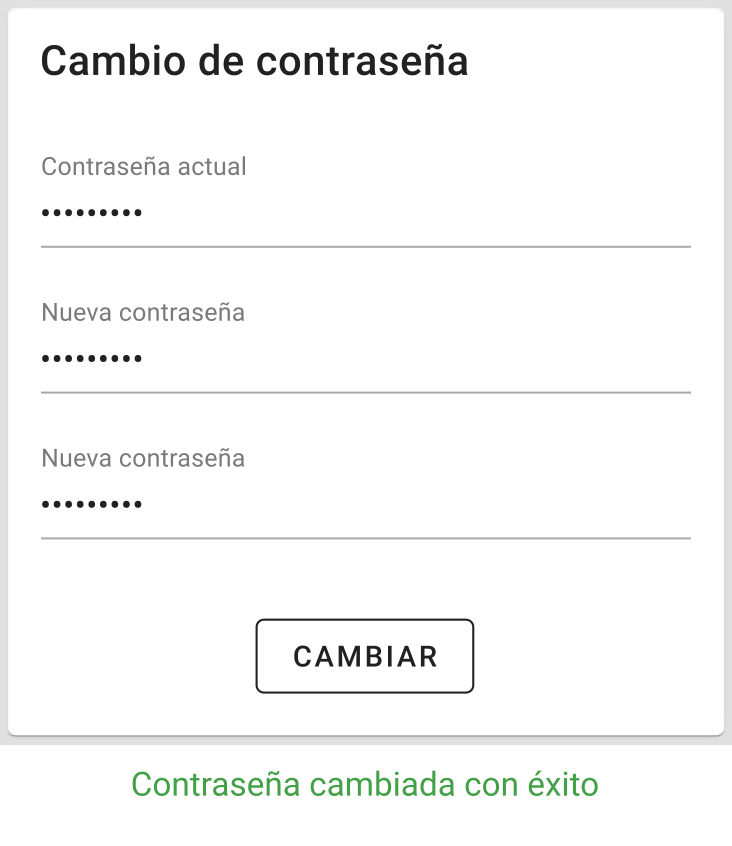
\includegraphics[width=\textwidth]{images/app/change-psw-sucess.png}
        \caption{Vista de cambio de contraseña realizado con exito}
        \label{fig:app-change-psw-success}
    \end{subfigure}
    % \caption{Vista de Cambio de contraseña (I)}
    \label{fig:app-change-psw-1}
\end{figure}
En caso de que la contraseña actual sea incorrecta se mostrará el mensaje de error  \textit{“Contraseña incorrecta”} (Figura~\ref{fig:app-change-psw_error-1}).
En caso de que las contraseñas nuevas no coincidan se mostrará el mensaje de error \textit{“Las contraseñas no coinciden”} (Figura~\ref{fig:app-change-psw_error-2})
\begin{figure}[H]
    \centering
    \begin{subfigure}[b]{0.45\textwidth}
        \centering
        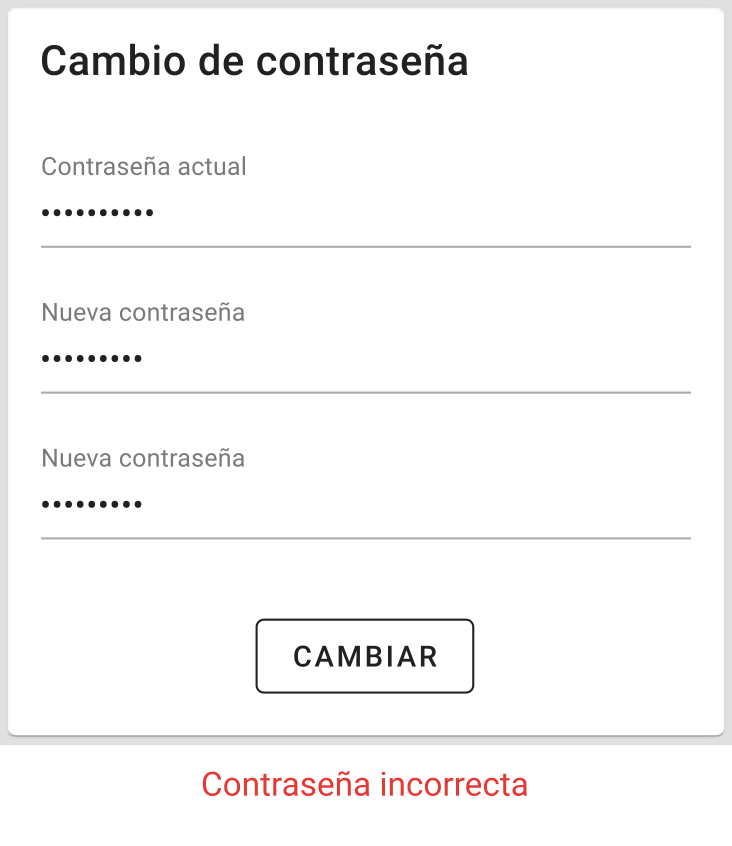
\includegraphics[width=\textwidth]{images/app/change-psw-error1.png}
        \caption{Vista de cambio de contraseña al ingresar contraseña incorrecta}
        \label{fig:app-change-psw_error-1}
    \end{subfigure}
    \hfill
    \begin{subfigure}[b]{0.45\textwidth}
        \centering
        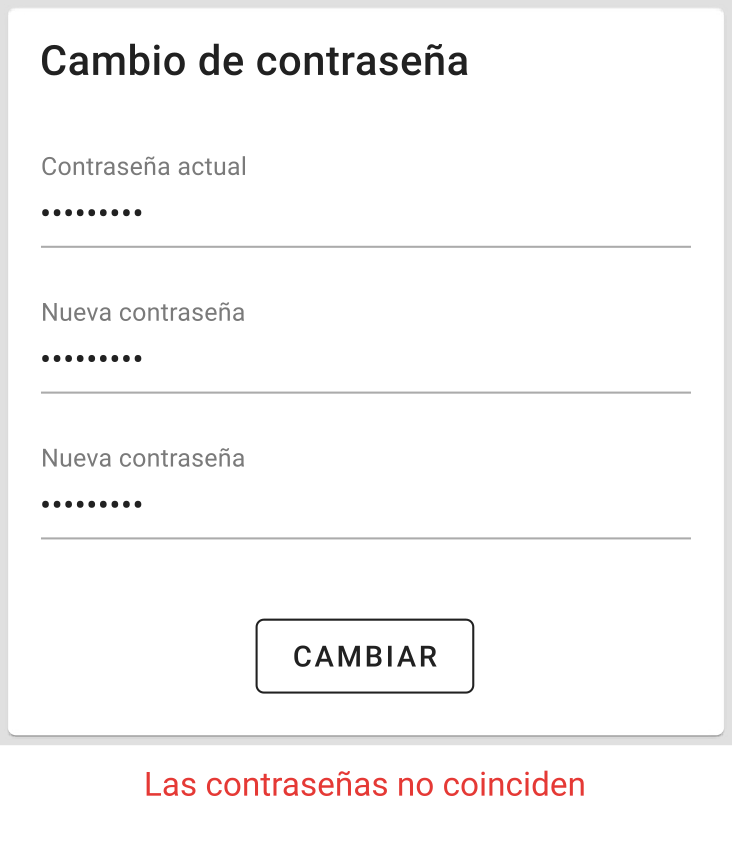
\includegraphics[width=\textwidth]{images/app/change-psw-error2.png}
        \caption{Vista de cambio de contraseña al ingresar contraseñas que no coinciden}
        \label{fig:app-change-psw_error-2}
    \end{subfigure}
    % \caption{Vista de Cambio de contraseña (II)}
    \label{fig:app-change-psw-2}
\end{figure}

En el caso de que la nueva contraseña no cumpla los críterios de seguridad (longitud mínima de 8 caracteres y al menos un número) se mostrará el mensaje de error  \textit{“La contraseña debe tener al menos 8 caracteres / La contraseña debe tener al menos un número”} (Figura~\ref{fig:app-change-psw_error-1}).
\begin{figure}[H]
    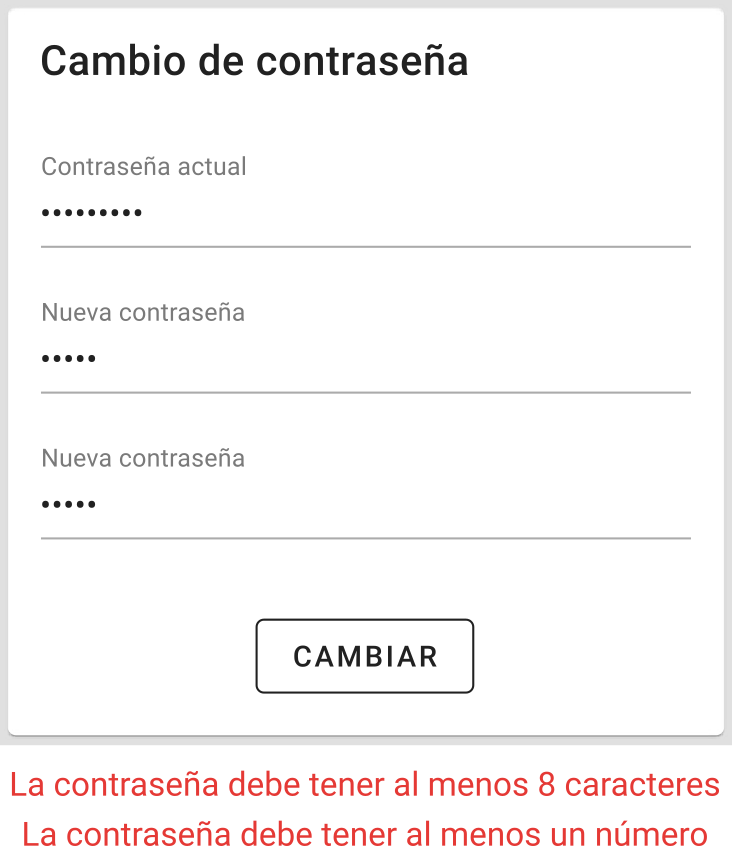
\includegraphics[width=0.45\linewidth]{images/app/change-psw-error3.png}
    \captionsetup{justification=raggedright, width=0.45\linewidth, singlelinecheck=off}

    % \captionsetup{width=0.45\linewidth}
    \caption{Vista de cambio de contraseña al ingresar una nueva contraseña que no cumple con los críterios de seguridad}
    \label{fig:app-change-psw_error-3}
\end{figure}

% \begin{figure}[H]
%     \centering
%     \begin{subfigure}[b]{0.4\textwidth}
%         \centering
%         \includegraphics[width=\textwidth]{images/app/chage-psw-def.png}
%         \caption{a}
%         \label{fig:subfig1}
%     \end{subfigure}
%     \hfill
%     \begin{subfigure}[b]{0.4\textwidth}
%         \centering
%         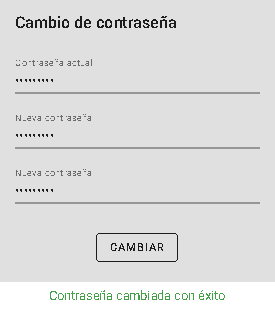
\includegraphics[width=\textwidth]{images/app/chage-psw-sucess.png}
%         \caption{b}
%         \label{fig:subfig2}
%     \end{subfigure}

%     \vskip\baselineskip

%     \begin{subfigure}[b]{0.4\textwidth}
%         \centering
%         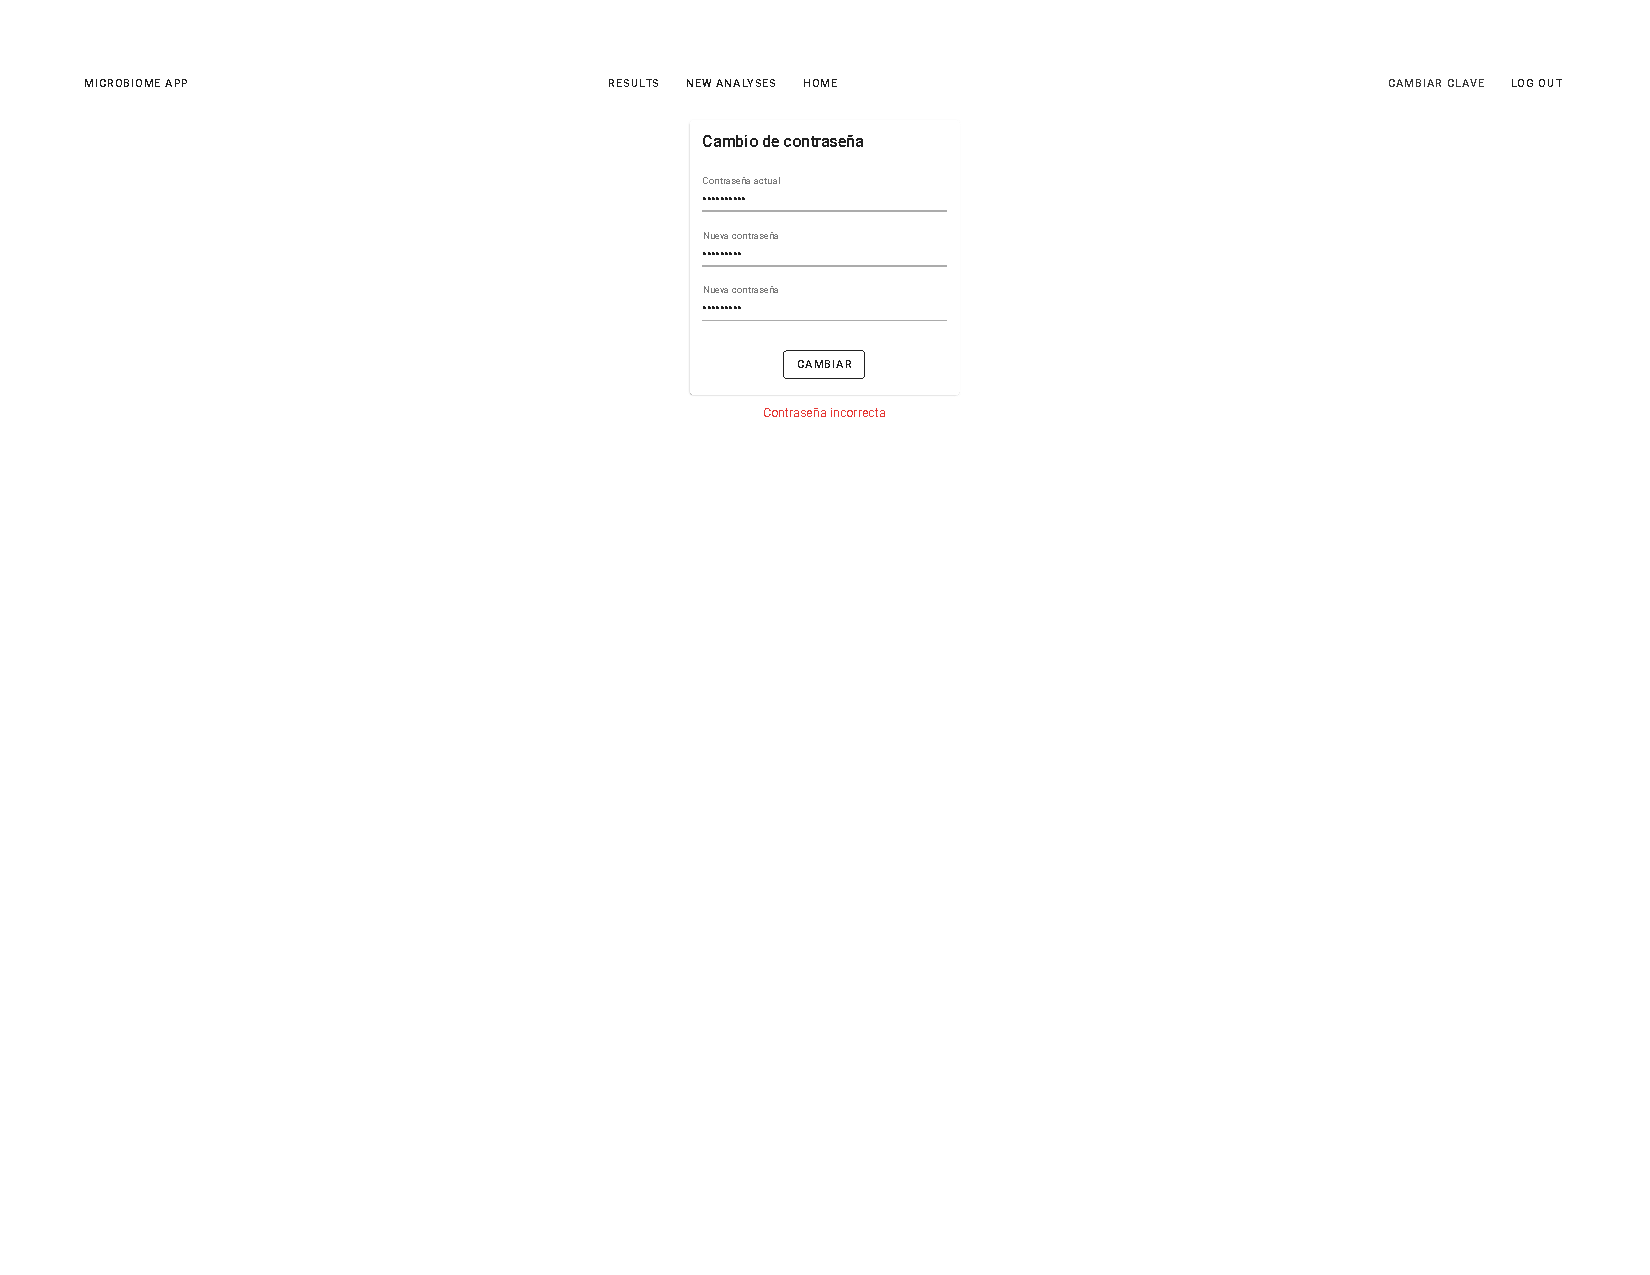
\includegraphics[width=\textwidth]{images/app/chage-psw-error1.png}
%         \caption{c}
%         \label{fig:subfig3}
%     \end{subfigure}
%     \hfill
%     \begin{subfigure}[b]{0.4\textwidth}
%         \centering
%         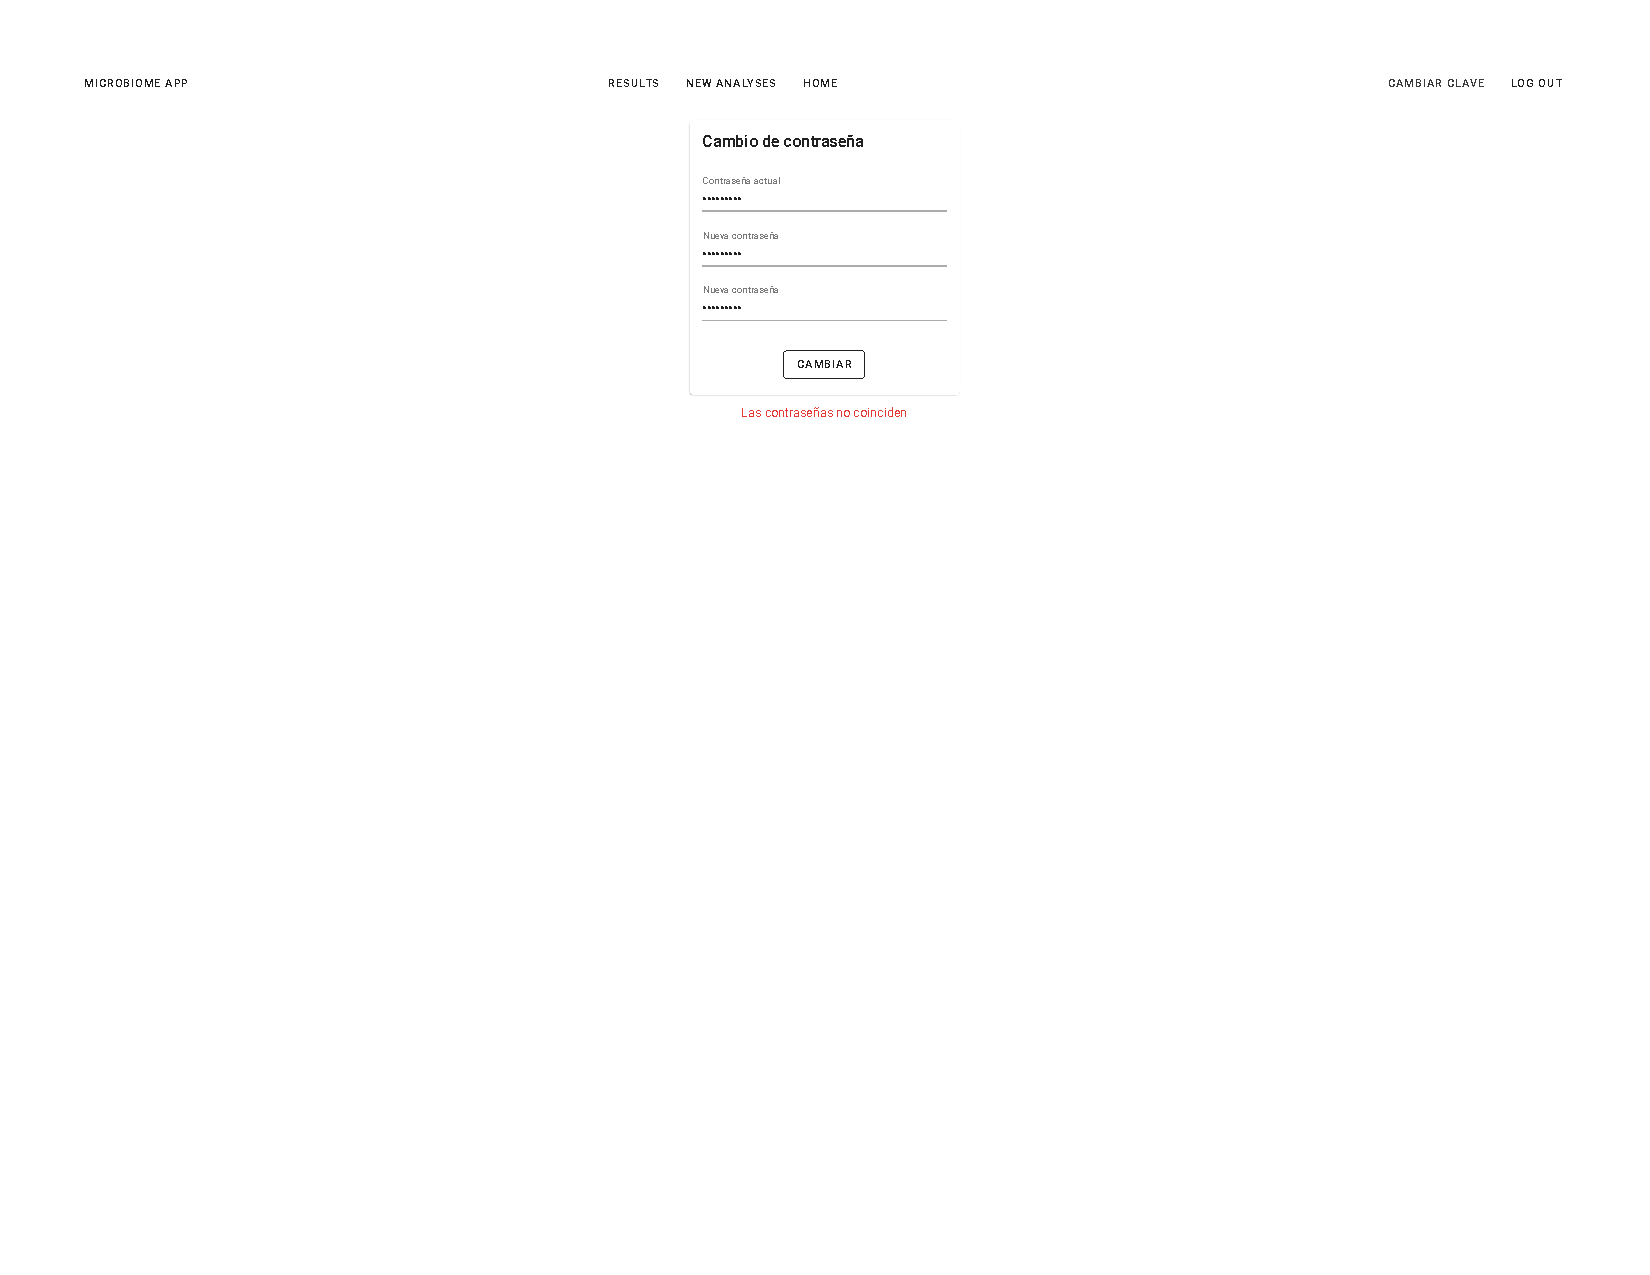
\includegraphics[width=\textwidth]{images/app/chage-psw-error2.png}
%         \caption{d}
%         \label{fig:subfig4}
%     \end{subfigure}

%     \vskip\baselineskip

%     \begin{subfigure}[b]{0.4\textwidth}
%         \centering
%         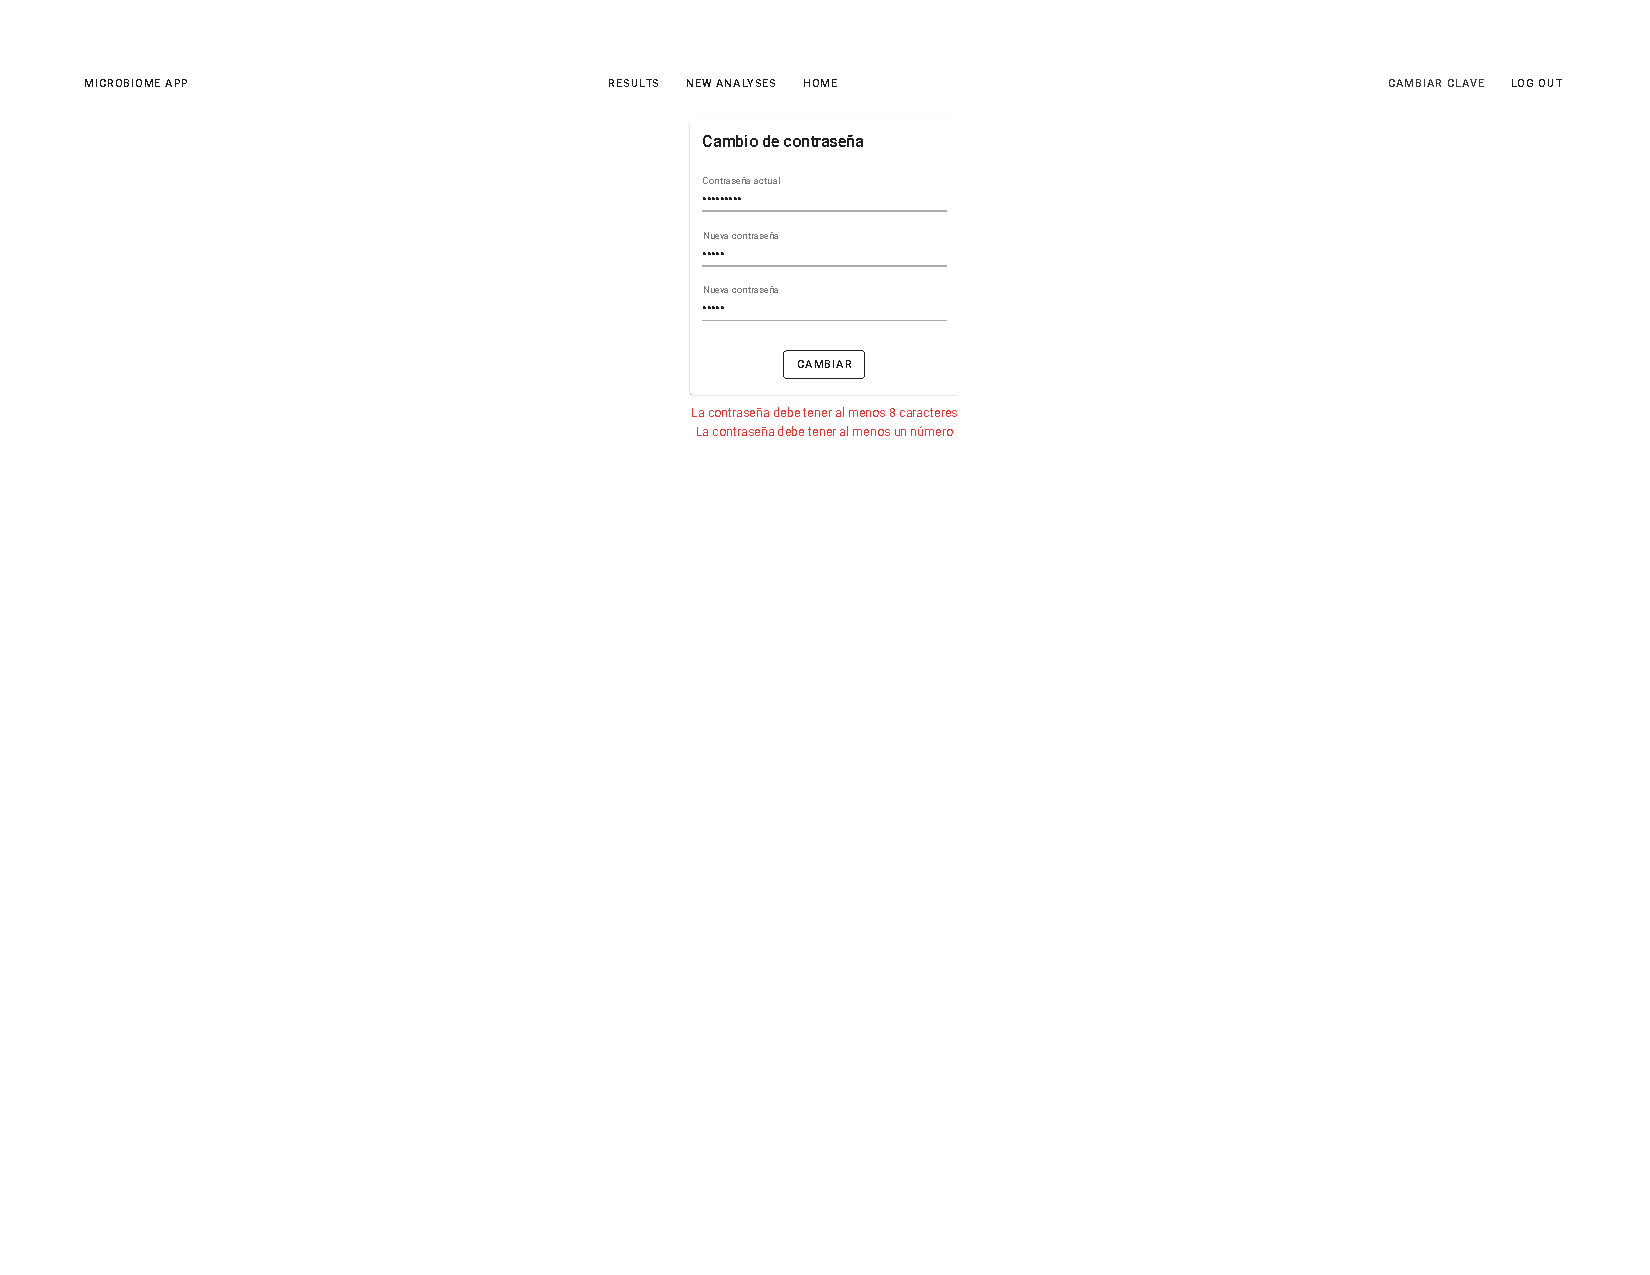
\includegraphics[width=\textwidth]{images/app/chage-psw-error3.png}
%         \caption{e}
%         \label{fig:subfig5}
%     \end{subfigure}
    
%     \caption{Título de la figura principal}
%     \label{fig:main}
% \end{figure}


\subsection{Nuevo análisis}
En esta sección el usuario deberá ingresar la información del proyecto, datos de secuenciación, y metadata para poder realizar los análisis. 
El usuario deberá rellenar la información básica del proyecto como, nombre, descripción, tipo de archivos y mediante un archivo en formato (XLXS) deberá ingresar la información de las muestras. %, como nombre de archivo, nombre de la muestra, barcode (opcional) y grupo (opcional).
Los datos de secuenciación se debe subir a algún directorio del drive del usuario y se debe dar acceso a la cuenta \textit{nanotax.catg@gmail.com}.
La figura~\ref{fig:app-new-analysis-def} presenta la vista inicial de la sección de Nuevo análisis.

\begin{figure}[H]
    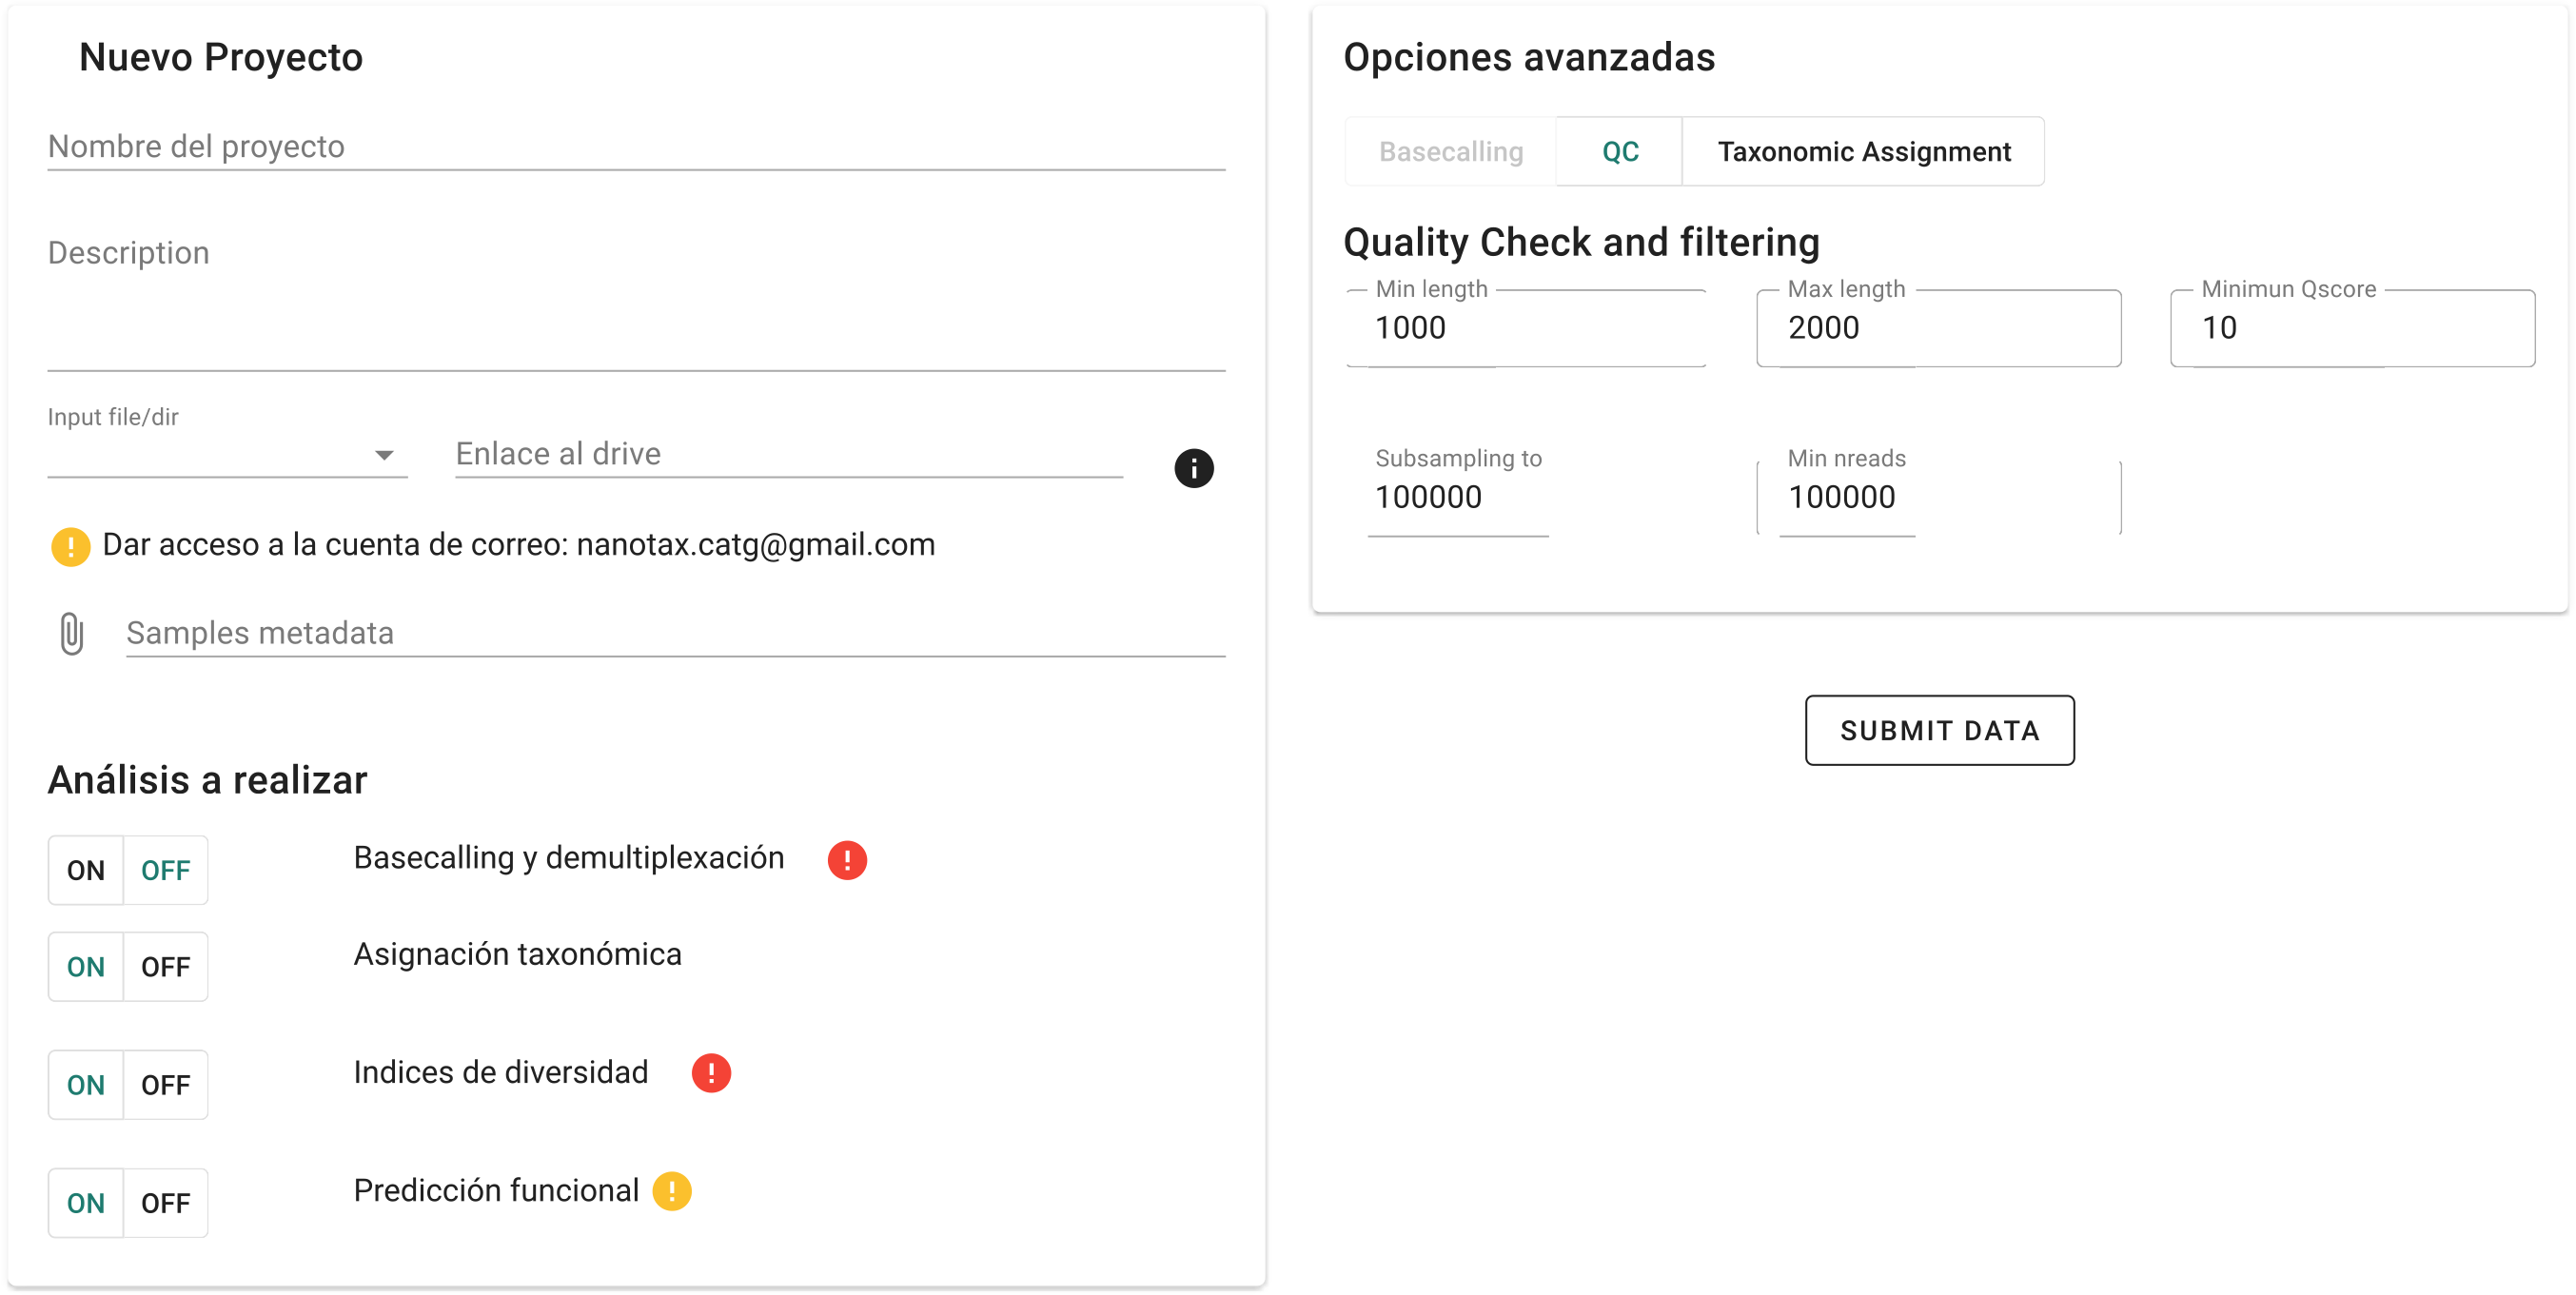
\includegraphics[width=1\linewidth]{images/app/newAnalysis/new-analysis-def.png}
    % \captionsetup{justification=raggedright, width=0.45\linewidth, singlelinecheck=off}

    % \captionsetup{width=0.45\linewidth}
    \caption{Vista por defecto de Nuevo análisis}
    \label{fig:app-new-analysis-def}
\end{figure}


A continuación se describen los datos que el usuario debe rellenar:

\begin{itemize}
    \item Nombre: Nombre del proyecto a utilizar en la plataforma (sección de visualización de proyectos y resultados).
    \item Descripción (opcional): Descripción del proyecto, campo opcional.
    \item Tipo de archivo a subir (POD5, FASTQ): Archivos de secuenciación que se procesarán:
    \begin{itemize}
        \item POD5: En caso de querer comenzar desde el proceso de basecalling y demultiplexación de las muestras.
        \item FASTQ: En caso de querer saltarse el paso de basecalling y demultiplexación e iniciar directamente con el control de calidad y asignación taxonómica.
    \end{itemize}
    \item Archivo de metadata en formato XLXS con las siguientes columnas para cada muestra:
    \begin{itemize}
        \item file: nombre del archivo subido al drive (obligatorio)
        \item sample: identificador de la muestra (obligatorio)
        \item barcode (opcional): barcode que identifica la muestra (en caso de querer realizar basecalling y demultiplexación)
        \item group (opcional): groupo al que pertenece cada muestra (en caso de querer hacer diferenciación entre grupos)
    \end{itemize}
    \item Análisis a realizar:
    \begin{itemize}
        \item Basecalling y demultiplexacion
        \item Asignación taxonomica
        \item Indices de diversidad
        \item Predicción funcional
    \end{itemize}
\end{itemize}


En el lado derecho de la vista se puede visualizar una sección de opciones avanzadas, donde el usuario puede modificar los parámetros por defecto en caso de que quiera modificar el comportamiento del pipeline (gigura~\ref{fig:app-new-analysis-def}). Esta información es seleccionados desde la base de datos la cual almacena los parámetros por defecto del flujo de trabajo.

Cabe destacar que en caso de que el directorio del drive no contenga la información necesaria, el proyecto se subirá correctamente y luego pasara a un estado de datos inválidos.
Los filtros y control de calidad se realizan siempre por lo que no aparecerá la opción en la lista de análisis.
Por defecto basecalling y demuliplexación se encuentra deshabilitado, en caso de que el usuario desee realizar este análisis deberá seleccionarlo, y al hacerlo se desbloqueará la sección de configuración de este análisis (Figura~\ref{fig:app-new-analysis-basecallingON}).



\begin{figure}[H]
    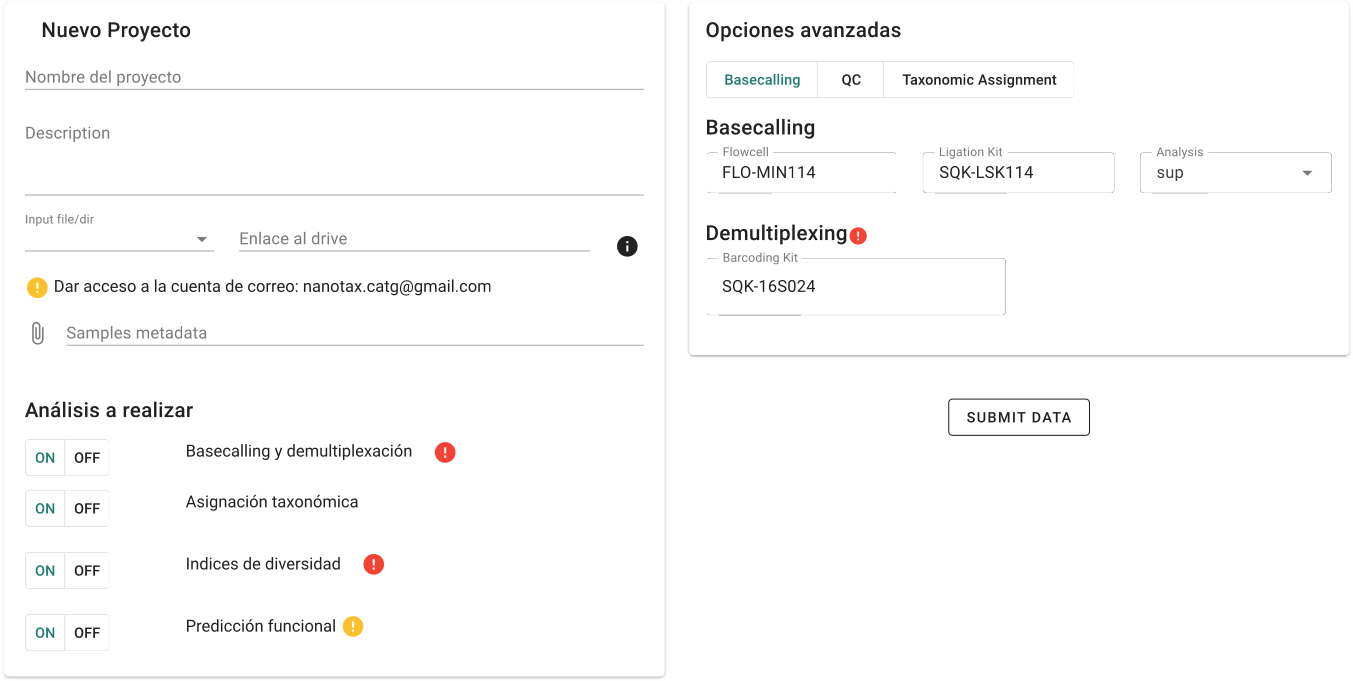
\includegraphics[width=1\linewidth]{images/app/newAnalysis/new-analysis-basecallingON.png}
    % \captionsetup{justification=raggedright, width=0.45\linewidth, singlelinecheck=off}

    % \captionsetup{width=0.45\linewidth}
    \caption{Vista de Nuevo análisis habilitando la opción de basecalling y demultiplexación}
    \label{fig:app-new-analysis-basecallingON}
\end{figure}
% La plataforma se encarga de verificar si el archivo de metadata cuenta con la información necesaria para realizar cada analisis. En caso de que el archivo de metadata no cuente con la información necesaria y el usuario desee realizar uno de esos analisis, se desplegara un mensaje de error al lado del análisis indicando que información se debe añadir en el archivo de metadata. Los parámetros que se pueden modificar son los siguientes:
% \begin{itemize}
%     \item Basecalling y demultiplexacion: Flowcell, kit de ligación y kit de barcoding utilizados durante la secuenciación. Modelo a utilizar para realizar el basecalling
%     \item QC: Longitud mínima y máxima en pares de bases de las lecturas, calidad mínima de las lecturas y cantidad de lecturas a utilizar para los análisis posteriores(subsampleo).
%     \item Predicción funcional: \hl{completar}
% \end{itemize}

% En la parte derecha del componente el usuario puede visualizar los parámetros por defecto y modificarlos en caso de que lo desee. 


Una vez que el usuario presione al botón \textit{Subir proyecto}, la plataforma realiza un proceso de validación para verificar que toda la información subida por el usuario sea correcta. En caso de no serla, la plataforma no permitirá subir el proyecto y podrá presentar alguno de los siguientes mensajes de error:
\begin{itemize}
    \item En caso de no completar el nombre del proyecto o el enlace al directorio del drive ambos campos pasarán a estar en color rojo (figura ~\ref{fig:app-new-analysis-type-file-error}).
    \item En caso de no seleccionar el tipo de archivo a subir, este campo pasará a estar en color rojo y se presentará el siguiente mensaje: \textit{Debe seleccionar el formato de los archivos de entrada} (figura ~\ref{fig:app-new-analysis-type-file-error}).
    \item En caso de seleccionar el formato de archivo \textit{POD5} y no haber seleccionado el proceso de basecalling y demultiplexación como inicio se presentará el mensaje: \textit{Al iniciar con basecalling debe subir los archivos POD5} (figura ~\ref{fig:app-new-analysis-type-file-error}).
    \item En caso de seleccionar el formato de archivo \textit{FASTQ} y haber seleccionado el proceso de basecalling y demultiplexación como inicio se presentará el mensaje: \textit{Al iniciar con QC o asignación taxonómica debe subir los archivos FASTQ} (figura ~\ref{fig:app-new-analysis-type-file-error}).
    \item En caso de que el archivo de metadata no cuente con todas las columnas necesarias se pueden presentar uno o más de los siguientes mensajes de errores (figura ~\ref{fig:app-new-analysis-type-file-error}):
    \begin{itemize}
        \item \textit{El archivo de metadata le falta la columna file}
        \item \textit{El archivo de metadata le falta la columna sample}
        \item \textit{El archivo de metadata le falta la columna barcode}: Solo en caso de seleccionar basecalling y demultiplexación como inicio del pipeline.
        \item \textit{El archivo de metadata le falta la columna group}: Solo en caso de querer realizar análisis por grupos (índices de diversidad).

    \end{itemize}
\end{itemize}


\begin{figure}[H]
    \centering
    \begin{subfigure}[b]{0.45\textwidth}
        \centering
        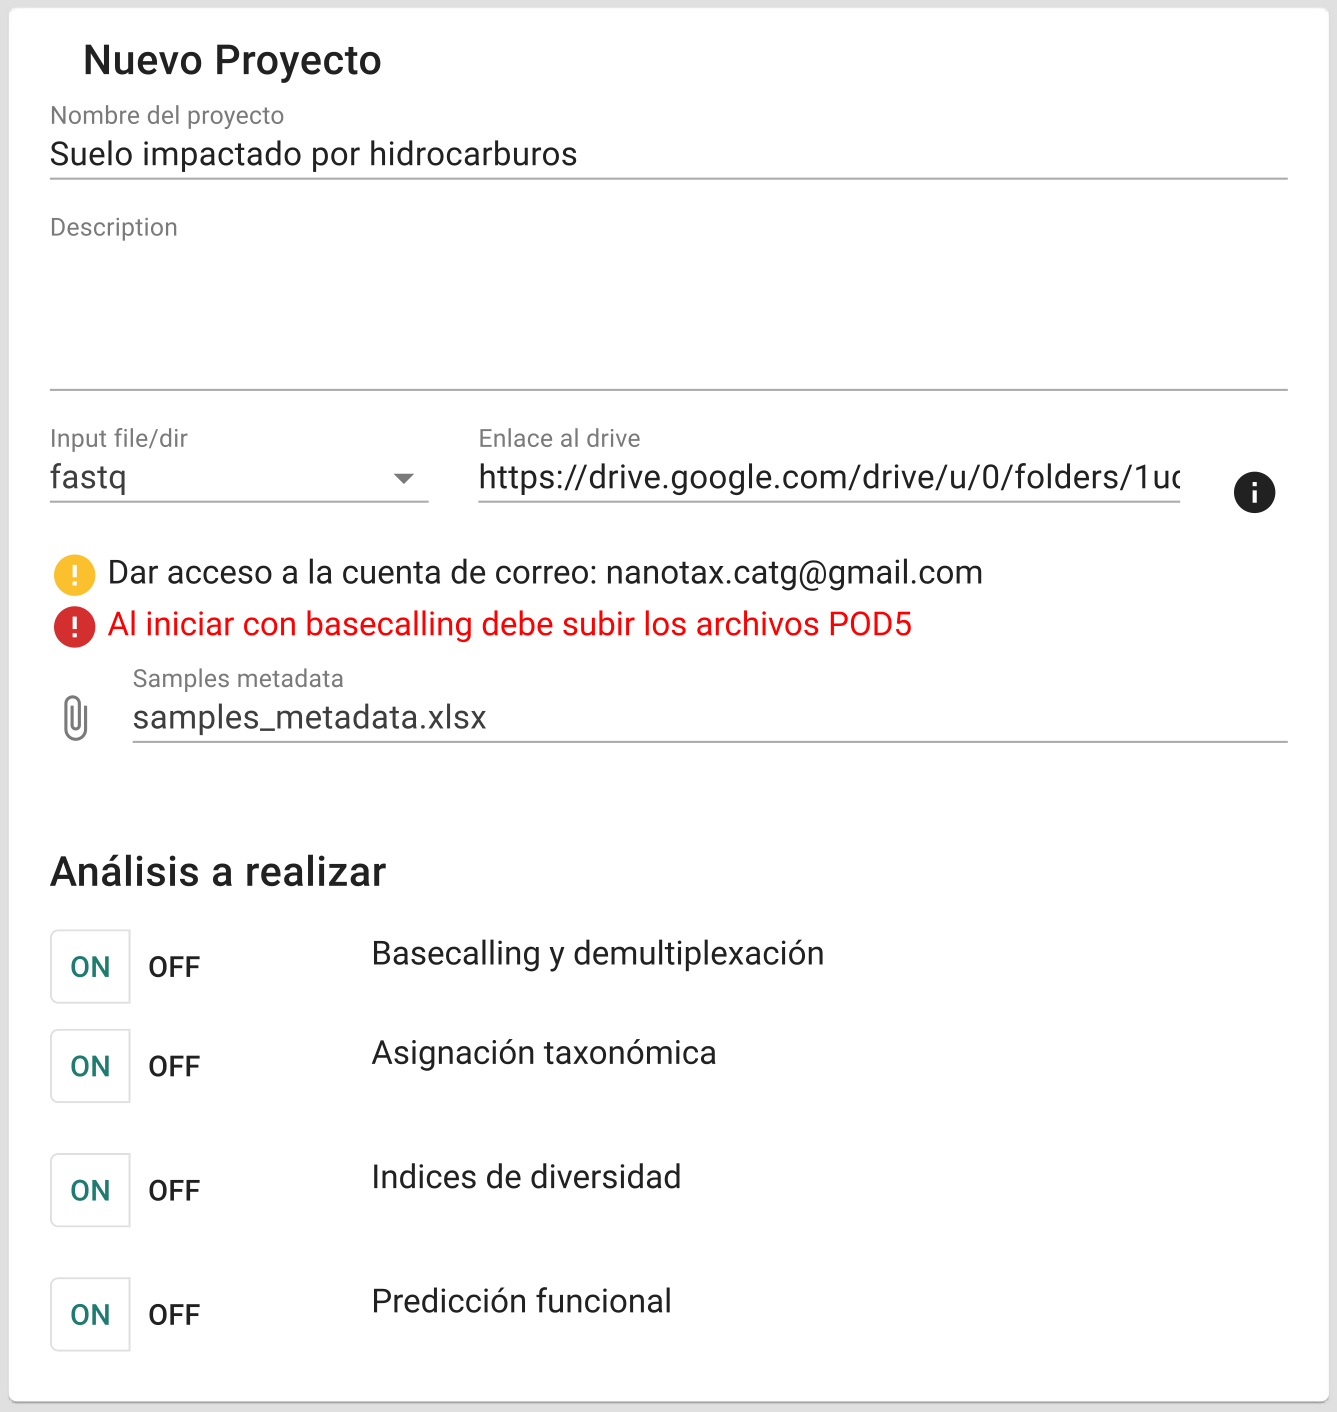
\includegraphics[width=\textwidth]{images/app/newAnalysis/pod5-error.png}
        \caption{Vista de nuevo análisis: Error al seleccionar el tipo del archivo}
        \label{fig:app-new-analysis-pod5-error}
    \end{subfigure}
    \hfill
    \begin{subfigure}[b]{0.45\textwidth}
        \centering
        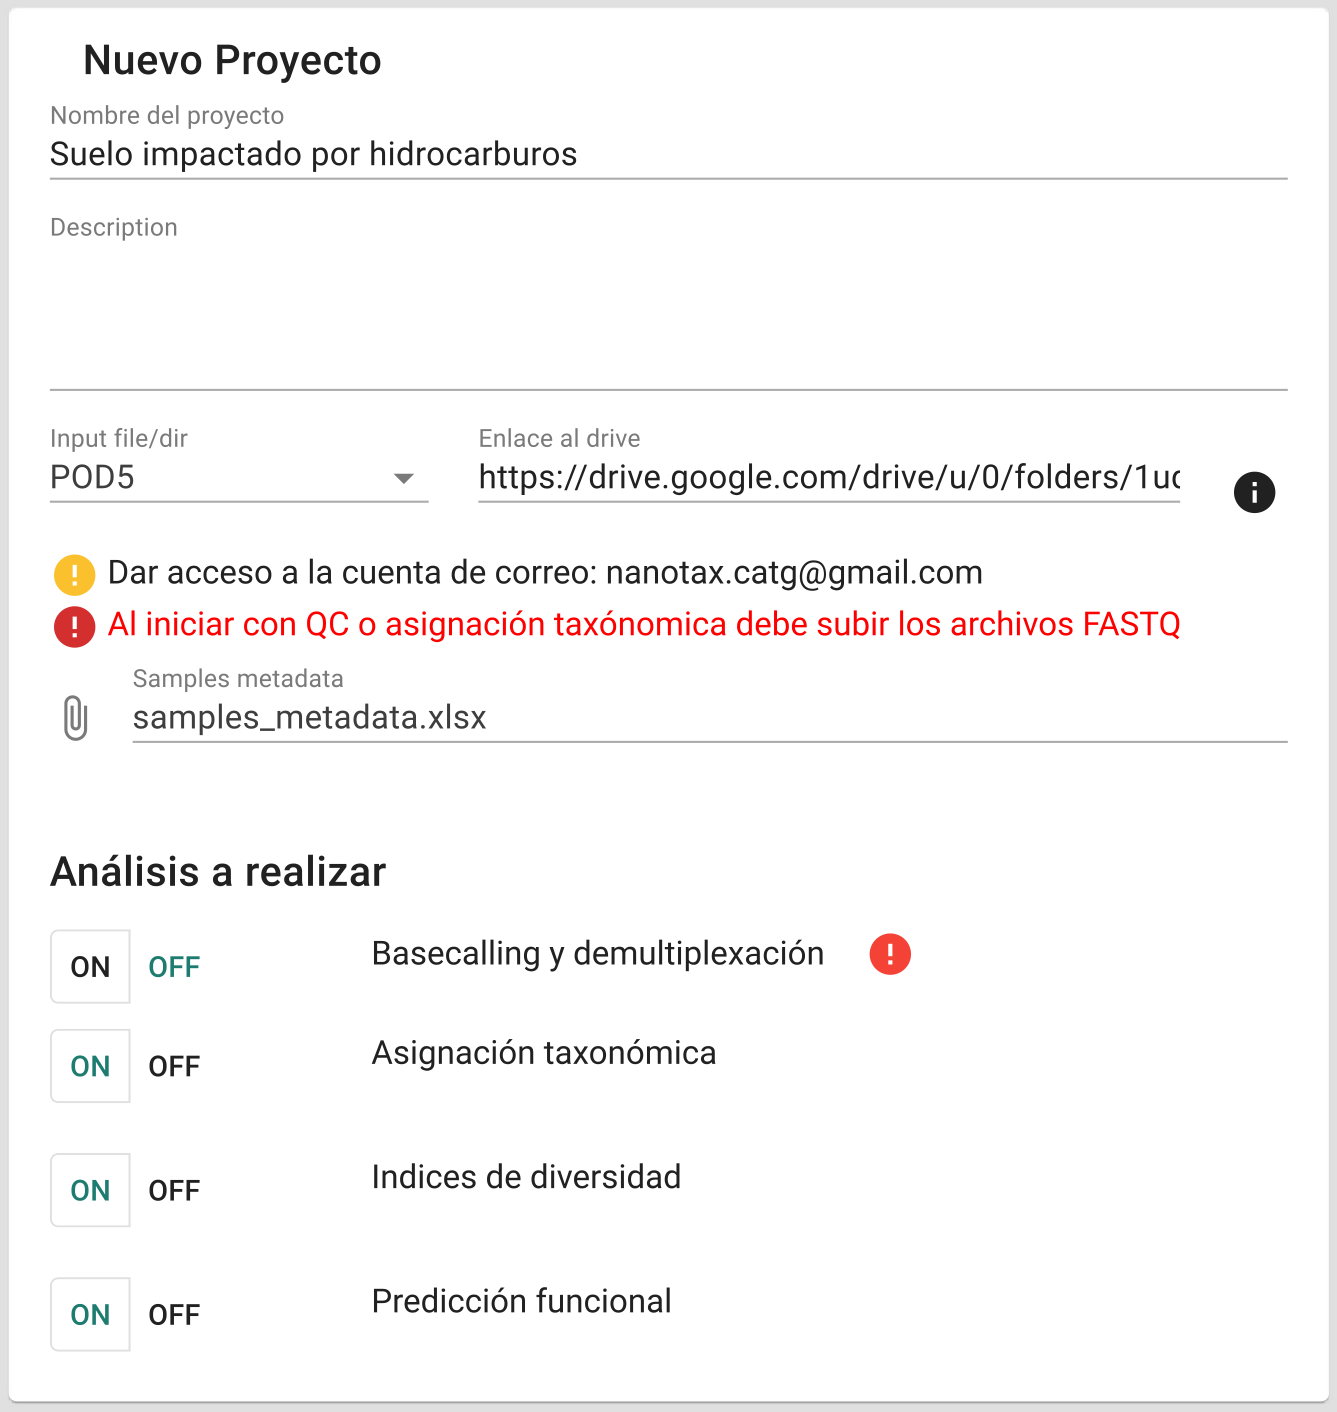
\includegraphics[width=\textwidth]{images/app/newAnalysis/fastq.png}
        \caption{Vista de nuevo análisis: Error al seleccionar el tipo del archivo}
        \label{fig:app-new-analysis-fastq-error}
    \end{subfigure}
    \caption{Vista de nuevo análisis: Error al seleccionar el tipo del archivo}
    \label{fig:app-new-analysis-type-file-error}
\end{figure}



\begin{figure}[H]
    \centering
    \begin{subfigure}[b]{0.45\textwidth}
        \centering
        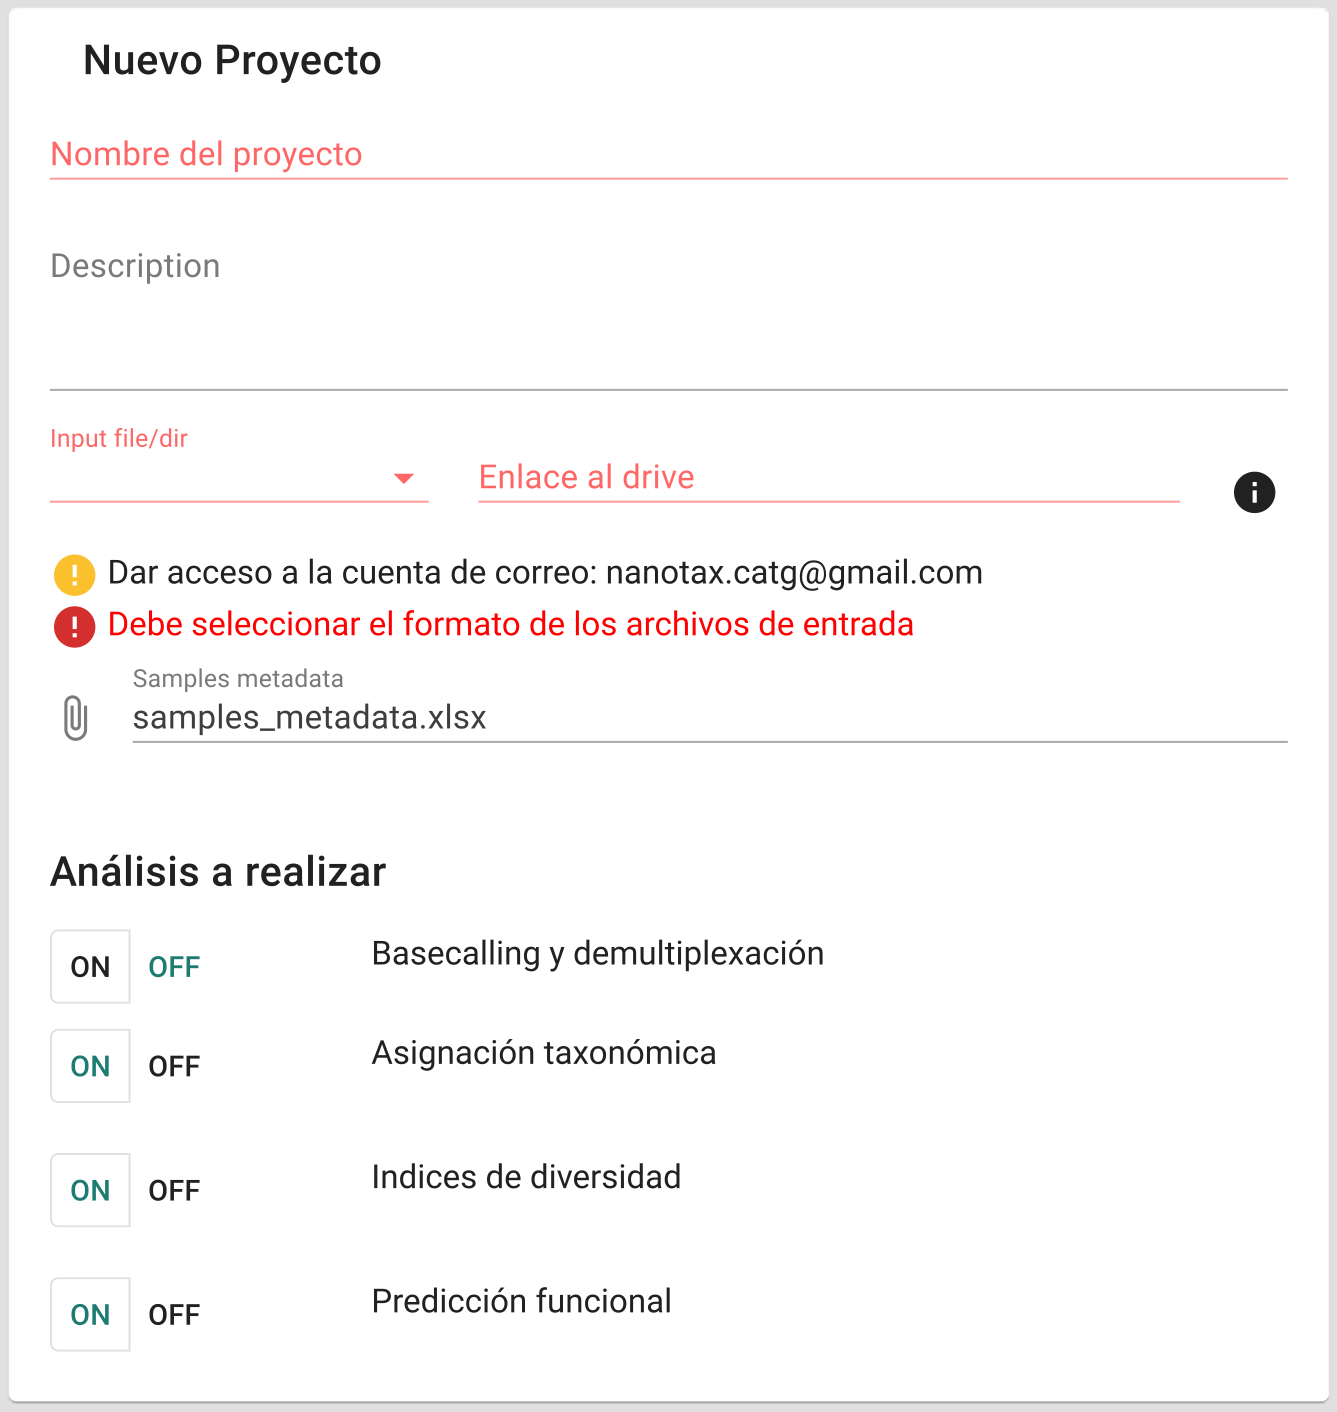
\includegraphics[width=\textwidth]{images/app/newAnalysis/errors1.png}
        \caption{Vista de nuevo análisis: Errores por falta de información}
        \label{fig:app-new-analysis-nodata-error}
    \end{subfigure}
    \hfill
    \begin{subfigure}[b]{0.45\textwidth}
        \centering
        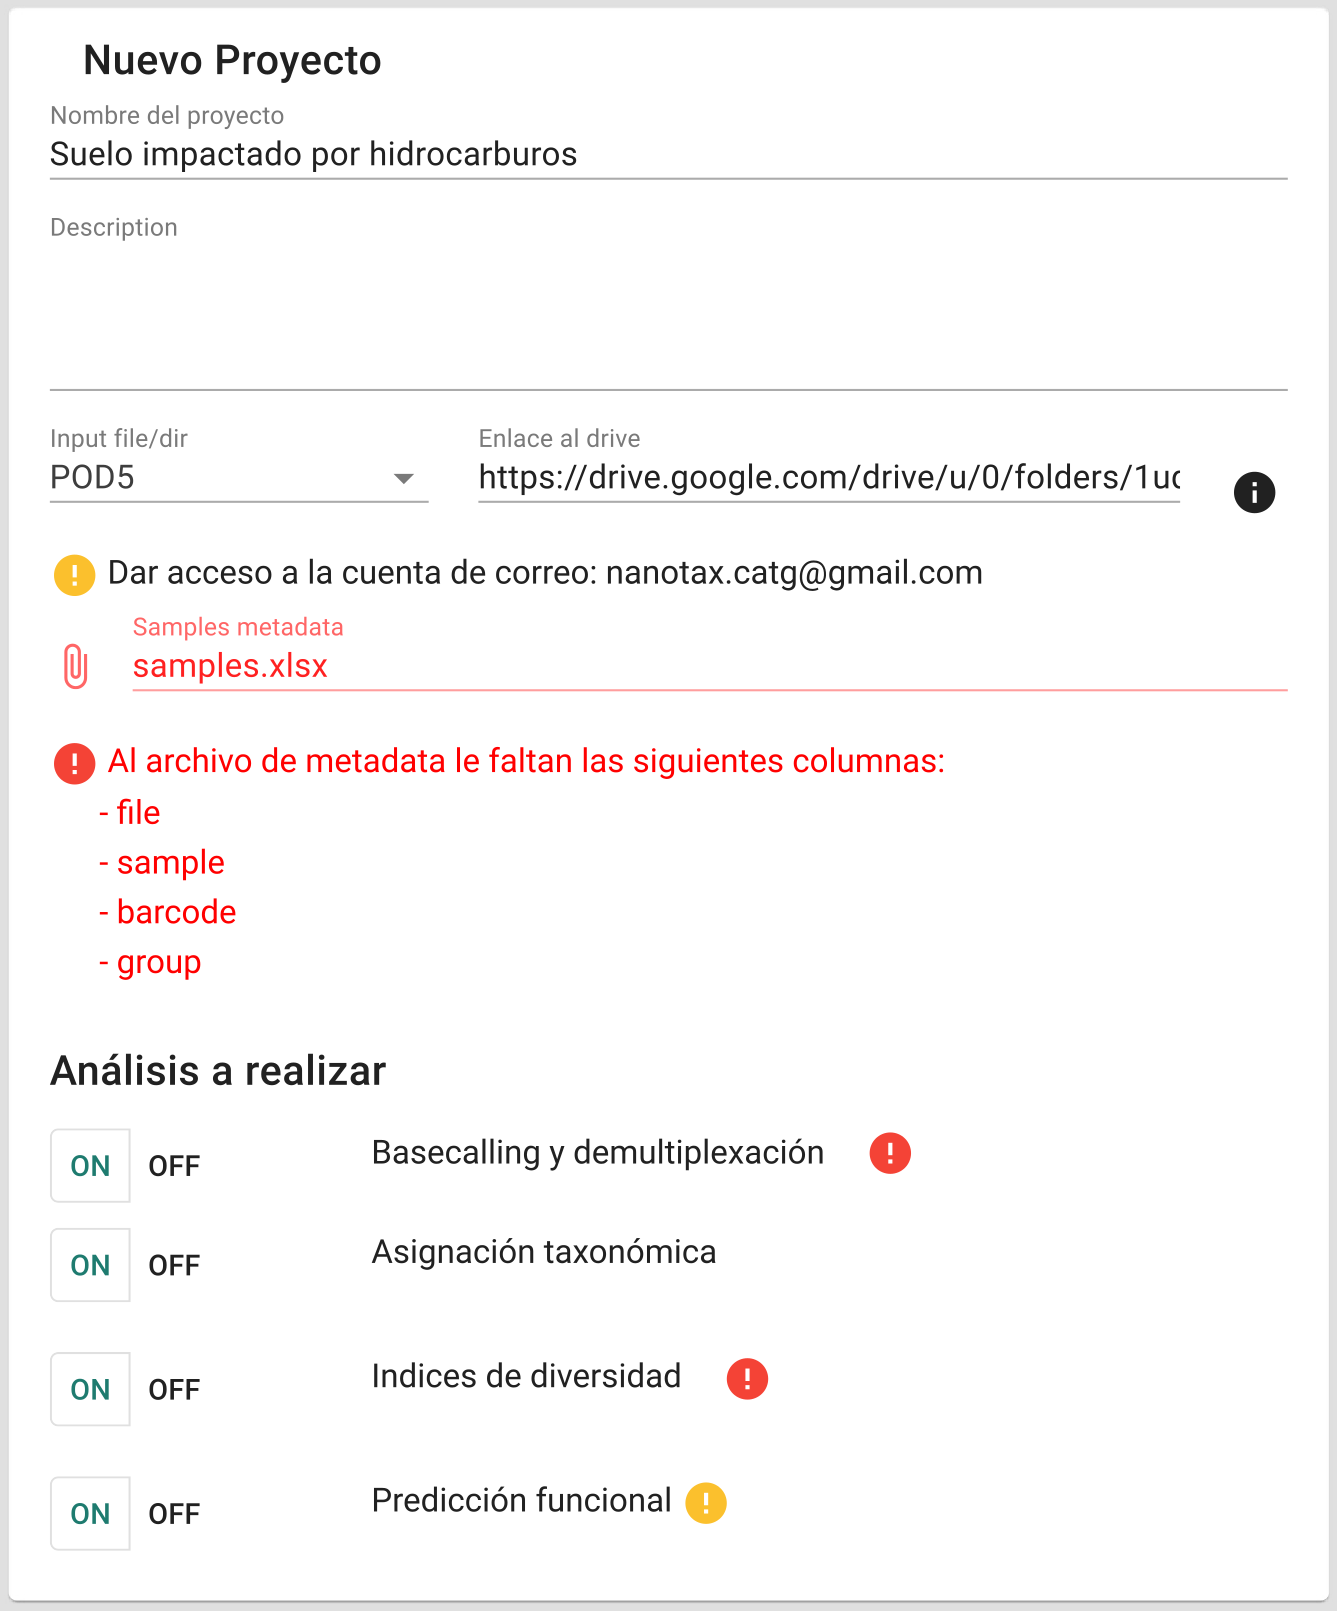
\includegraphics[width=\textwidth]{images/app/newAnalysis/metadata-error-1.png}
        \caption{Vista de nuevo análisis: Errores en el archivo de metadata}
        \label{fig:app-new-analysis-metadata-error}
    \end{subfigure}
    \caption{Vista de nuevo análisis: Errores }
    \label{fig:app-new-analysis-metadata-nodata-error}
\end{figure}



En la parte inferior del componente se encuentra el botón de Subir data, el cual al hacer click en el, ingresará la información a la base de datos y copiará los archivos a la plataforma de computo. Una vez que el usuario presionar el botón de subir data, la plataforma se encarga de verificar que se cuente con toda la información necesaria para correr el pipeline.





%%%%%%%%%%%%%%%%%%%%%%%%%%%%%%%%%%%%%%%%%%%%%%%%%%%%%%%%%%%%%%%%%%%%%%

\subsection{Resultados/Proyectos} \label{projects}
Una vez que el usuario valida sus credenciales en la plataforma será redireccionado a la sección de Resultados. En esta sección se mostraran los proyectos que el usuario ha subido a la plataforma, estos proyectos pueden estar en ejecución, finalizados o finalizados con errores. 
Por cada proyecto se desplegará la información básica en una tarjeta:
\begin{itemize}
    \item Nombre del proyecto
    \item Descripción del proyecto
    \item Cantidad de muestras procesadas, descartadas y totales
    \item Estado del proyecto (corriendo, finalizado, subido con errores)
    \item En caso de que el proyecto haya finalizado el usuario podrá acceder a la sección especifica de resultados del proyecto mediante el botón de Ver resultados.
\end{itemize}

A continuación se presenta un ejemplo de la vista de proyectos subidos a la plataforma (Figura~\ref{fig:app-results-projects}).
El primer proyecto se encuentra \textit{corriendo} por lo que no se tiene acceso a los resultados (botón de de ver resultados) ni a la información de las muestras descartadas ni analizadas correctamente.
El segundo proyecto se encuentra finalizado, por lo que se puede acceder a los resultados y se puede visualizar además la cantidad de muestras procesadas, descartadas y totales. 

\begin{figure}[H]
    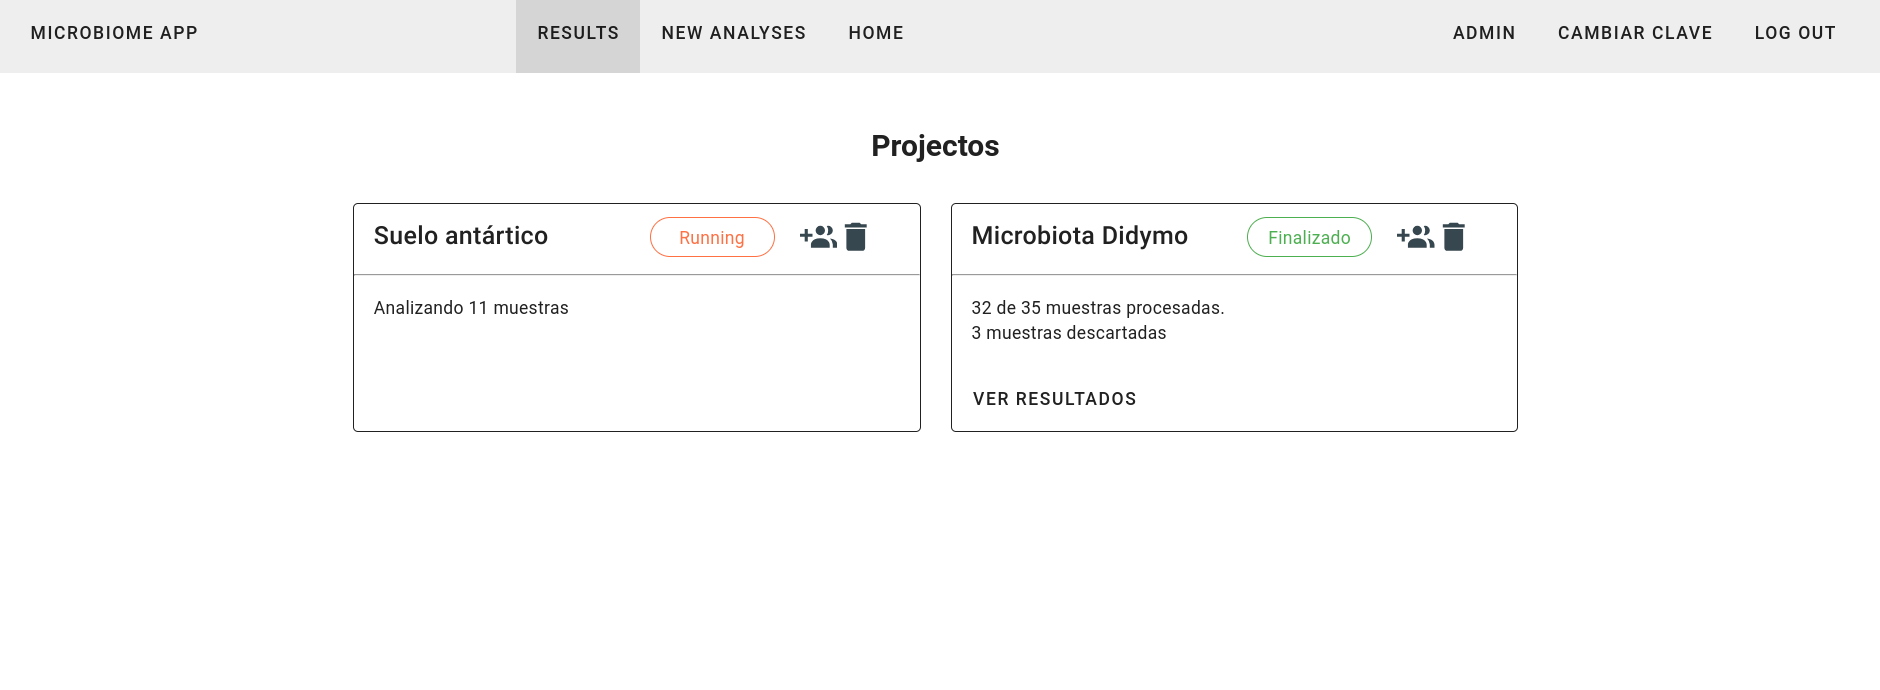
\includegraphics[width=1\linewidth]{images/app/projects.png}
    % \captionsetup{justification=raggedright, width=0.45\linewidth, singlelinecheck=off}

    % \captionsetup{width=0.45\linewidth}
    \caption{Vista de proyectos subidos a la plataforma}
    \label{fig:app-results-projects}
\end{figure}
En la parte superior de la tarjeta del proyecto se pueden visualizar dos íconos, uno para eliminar el proyecto y otro para poder compartir los resultados del proyecto con otros usuarios de la plataforma.


En el caso de seleccionar el botón para añadir usuarios se desplegará una ventana emergente donde se podrá ingresar el nombre de usuario al que se desea compartir los resultados del proyecto(Figura~\ref{fig:app-add-project}). 
En caso de que el usuario no exista en la plataforma se mostrará un mensaje de error \textit{“Usuario no encontrado”} (Figura~\ref{fig:app-add-project-invalid-usar}).
\begin{figure}[H]
        \centering
        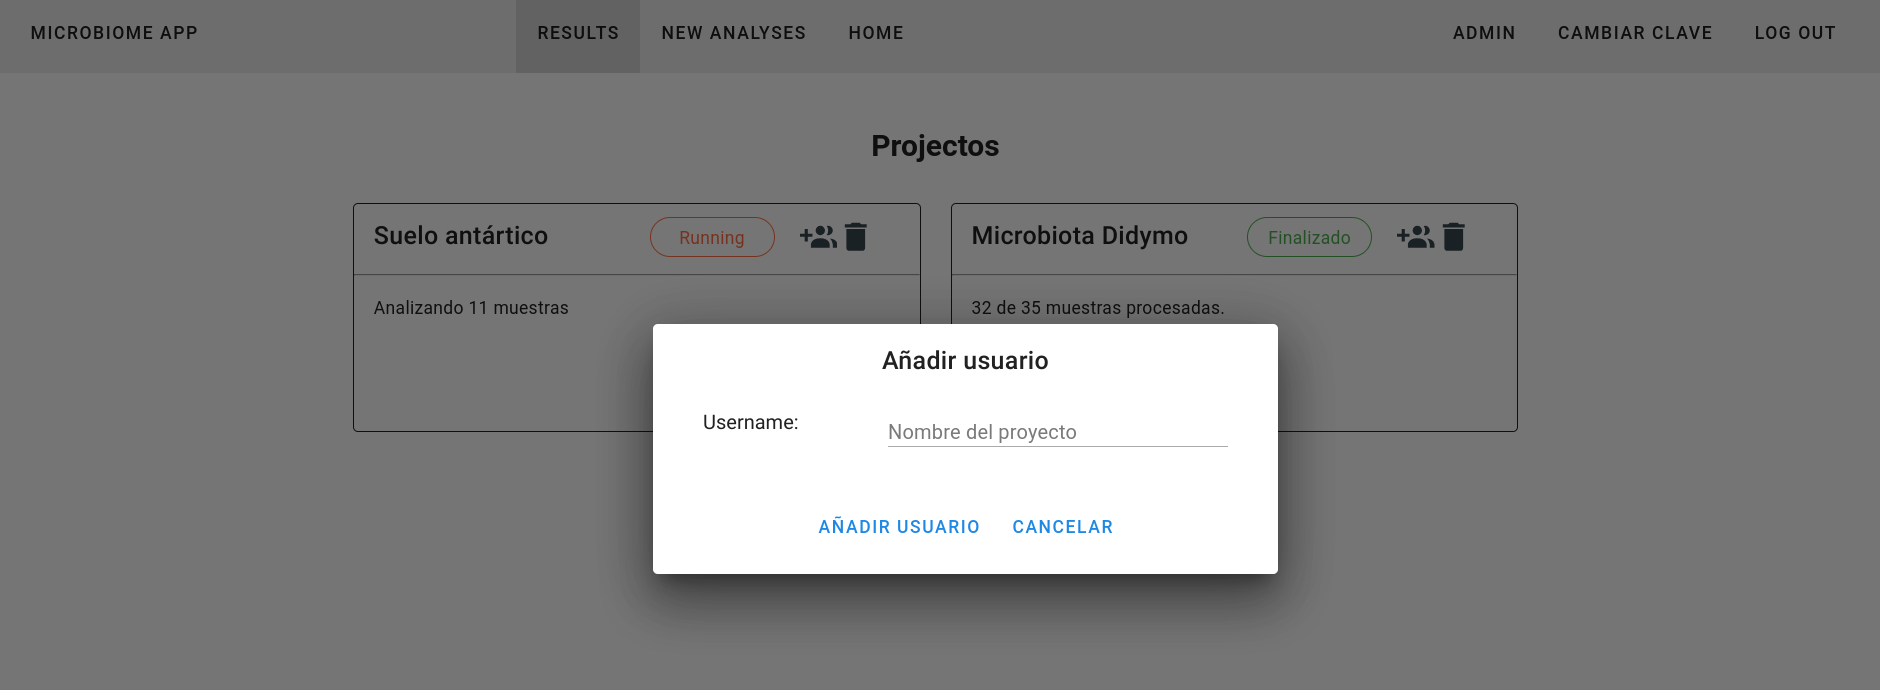
\includegraphics[width=\textwidth]{images/app/addUser.png}
        \caption{Añadir usuario a un proyecto existente}
        \label{fig:app-add-project}

\end{figure}

\begin{figure}[H]
    \centering
    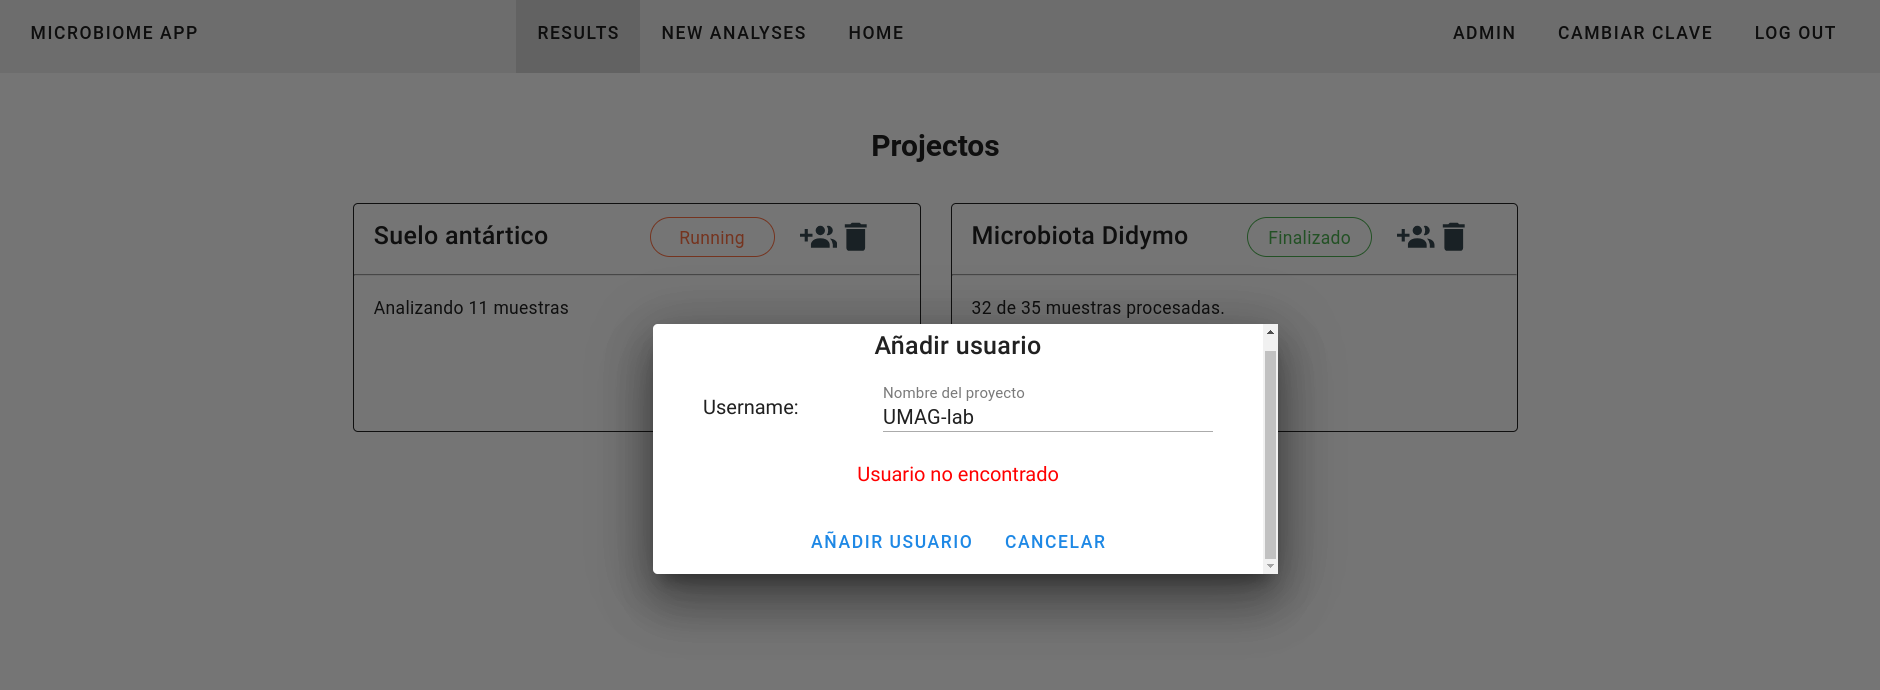
\includegraphics[width=\textwidth]{images/app/addUser_notFound.png}
    \caption{Añadir usuario a un proyecto existente: Mensaje de error debido a que el usuario no existe en la plataforma}
    \label{fig:app-add-project-invalid-usar}

\end{figure}

En el caso de seleccionar el icono para eliminar el proyecto se desplegará una ventana emergente con un mensaje de confirmación, en caso de confirmar la eliminación del proyecto se eliminará toda la información asociada al proyecto de la base de datos y se eliminarán los archivos asociados al proyecto de la plataforma de computo~\ref{fig:app-delete-project}.

\begin{figure}[H]
    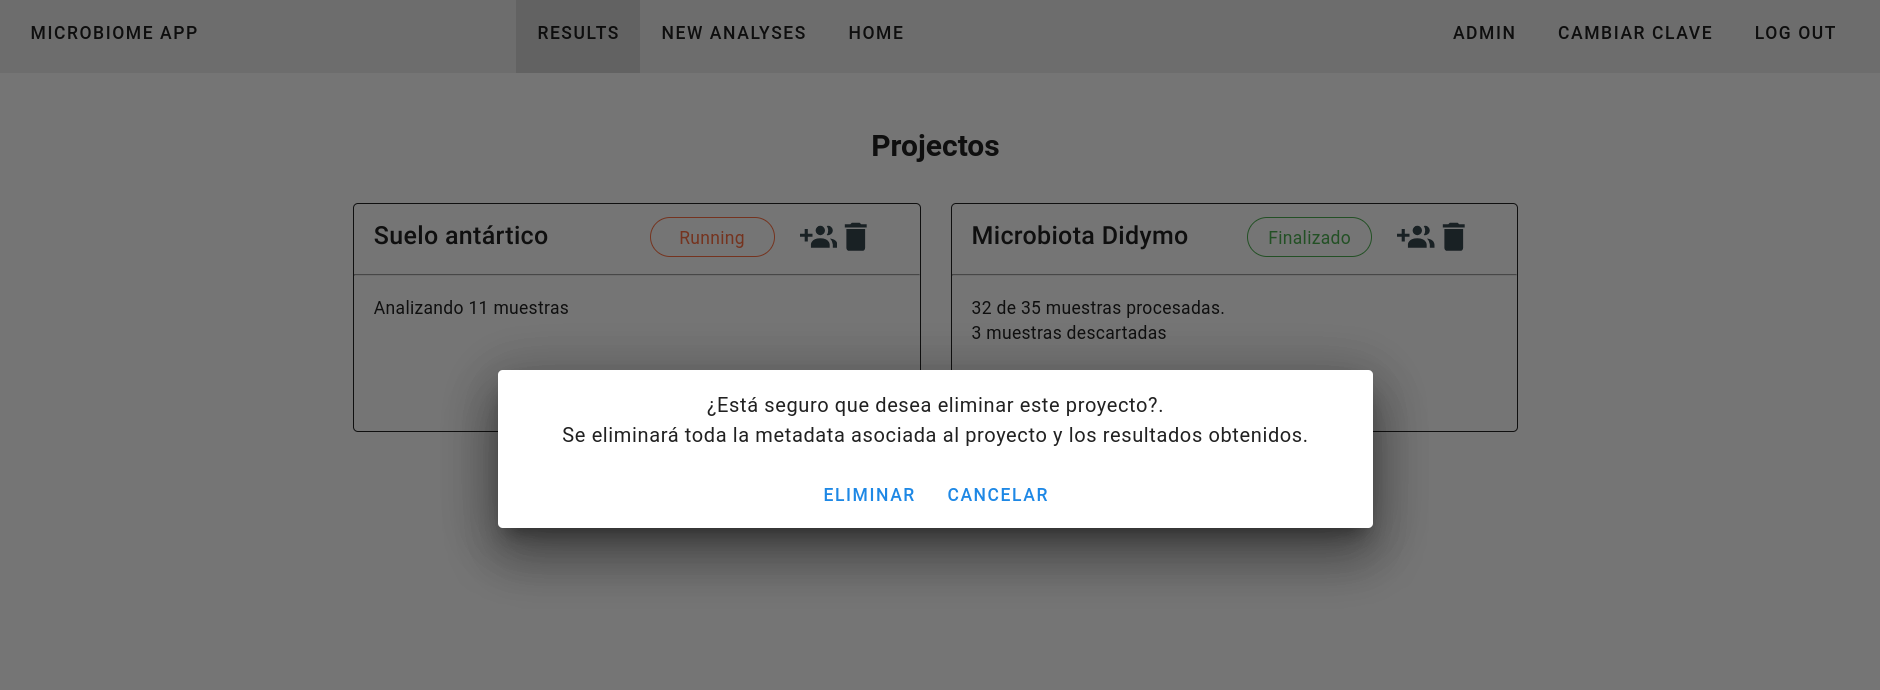
\includegraphics[width=1\linewidth]{images/app/deleteProject.png}
    % \captionsetup{justification=raggedright, width=0.45\linewidth, singlelinecheck=off}

    % \captionsetup{width=0.45\linewidth}
    \caption{Eliminar proyecto de la plataforma}
    \label{fig:app-delete-project}
\end{figure}

\subsection{Resultados de un proyecto en especifico}
Una vez que el pipeline haya finalizado su ejecución, la plataforma permitirá al usuario acceder a los resultados de cada proyecto leyendo los resultados desde la base de datos y desplegando la información en la sección de resultados de cada proyecto.
Esta sección cuenta con 5 subsecciones, cada una con información específica del análisis realizado. 
En caso de que al ingresar el proyecto el usuario no seleccione todos los análisis, solo se mostrarán las secciones indicadas por el usuario.

\subsection{Información básica de las muestras}
%Esta sección se mostrará siempre que el usuario empiece con archivos POD5 o FastQ, es decir, ya sea comenzando el análisis desde el basecalling o desde el control de calidad. \hl{Igual si es que solo se hace asignaicón taxonomica}.
Esta sección se desplegará siempre en la plataforma y cuenta en el lado izquierdo con una tabla con información básica de las muestras y en el lado derecho un gráfico que representa la calidad y tamaño promedio de las lecturas.
La tabla esta compuesta por los siguientes elementos:
\begin{itemize}
    \item Nombre de la muestra: Nombre indicado en el archivo de metadata al ingresar el proyecto.
    % \item \hl{Grupo}: Grupo asociado a la muestra en el archivo de metadata (en caso de ingresar grupo).
    \item Total de lecturas: Cantidad de lecturas previo a los filtros de calidad.
    \item Calidad promedio: Calidad promedio en formato phred despues de los filtros de calidad.
    \item Largo promedio: Largo promdio despues de los filtros de calidad
    \item Lecturas después de los filtros: Cantidad de lecturas luego de los filtros de calidad.
    \item Nota: Si la muestra fue descartada por no contar con la cantidad suficiente de lecturas se informará en esta columna.
\end{itemize}
En la parte inferior de la tabla hay una nota que indica la cantidad de lecturas que se consideraron para los análisis posteriores, este valor por defecto es 100.000, pudiendo ser modificado por el usuario en las opciones avanzadas al ingresar el proyecto.

En la parte derecha de la sección se puede visualizar un heatmap donde en el eje X se encuentra el tamaño de las secuencias, y en el eje Y la calidad. 
El color indica la cantidad de lecturas que se encuentran en esa intersección, mientras más intenso el color, más secuencias tienen la calidad y tamaño indicado.
Para este grafico se consideraron todas las muestras con sus lecturas después de los filtros de calidad.

% En la parte inferior del gráfico hay una nota que indica en que rangos de tamaño se encuentran la mayoria de las lecturas\hl{Muy generico?}. 
A continuación se presenta un ejemplo de la sección de información básica de las muestras (Figura~\ref{fig:app-results-basicStatistics}).
\begin{figure}[H]
    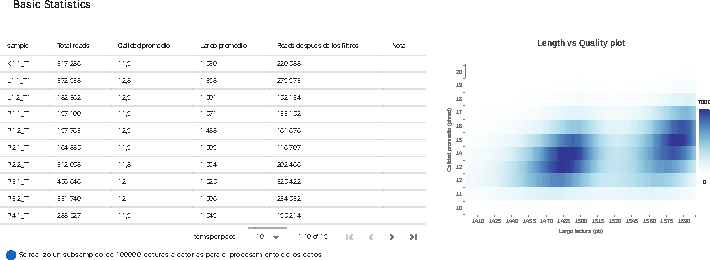
\includegraphics[width=1\linewidth]{images/app/results/basicStatistics.pdf}
    % \captionsetup{justification=raggedright, width=0.45\linewidth, singlelinecheck=off}

    % \captionsetup{width=0.45\linewidth}
    \caption{Estadisticas básicas (resultados)}
    \label{fig:app-results-basicStatistics}
\end{figure}

En caso de que el usuario ingrese un valor mínimo de lecturas para realizar los análisis y alguna de las muestras no cumpla con este valor, se mostrará un mensaje de error en la tabla de información básica de las muestras (Figura~\ref{fig:app-results-basicStatistics-exclude}).
\begin{figure}[H]
    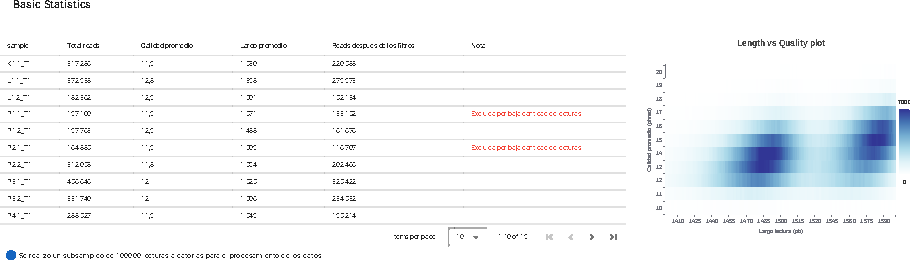
\includegraphics[width=1\linewidth]{images/app/results/basicStatistics_exclude.pdf}
    % \captionsetup{justification=raggedright, width=0.45\linewidth, singlelinecheck=off}

    % \captionsetup{width=0.45\linewidth}
    \caption{Estadisticas básicas (resultados)}
    \label{fig:app-results-basicStatistics-exclude}
\end{figure}

\subsection{Asignación taxonómica}
En la parte superior de esta sección se pueden visualizar pestañas que representan cada categoría taxonómica (especie, género, familia, orden, clase y filo), las cuales permiten ajustar la visualización de la información presentada en esta  sección (gráfico de barras apiladas y tabla). Por defecto se presenta la información para la categoría de especie.

Debajo de las pestañas en el lado izquierdo hay un gráfico de barras apiladas que permite visualizar la abundancia de las taxonomías en cada muestra.
El usuario puede interactuar con el gráfico modificando la visualización a través de los botones que se encuentran en la parte inferior, pudiendo visualizar la información en porcentaje o en cantidad de lecturas, como también pudiendo modificar el porcentaje mínimo para crear la categoria \textit{Otros}.
En caso de que el usuario hubiera ingresado información de grupos asociados a las muestras, se podrá visualizar un nuevo grupo de botones que permite al usuario visualizar la información de las taxonomías por grupo o por muestra.
La leyenda del gráfico de barras apiladas presenta solo las 10 taxonomías con mayor abundancia. 
Por defecto, todas aquellas taxonomías que tengan un valor menor al 0.01\% de abundancia serán eliminadas y aquellas con un porcentaje menor a un 1\%  serán agrupadas en una nueva taxonomia llamada \textit{Otros}.


A continuación se puede visualizar como se presenta la sección de taxonomía en la plataforma (Figura~\ref{fig:app-results-taxonomy}).

\begin{figure}[H]
    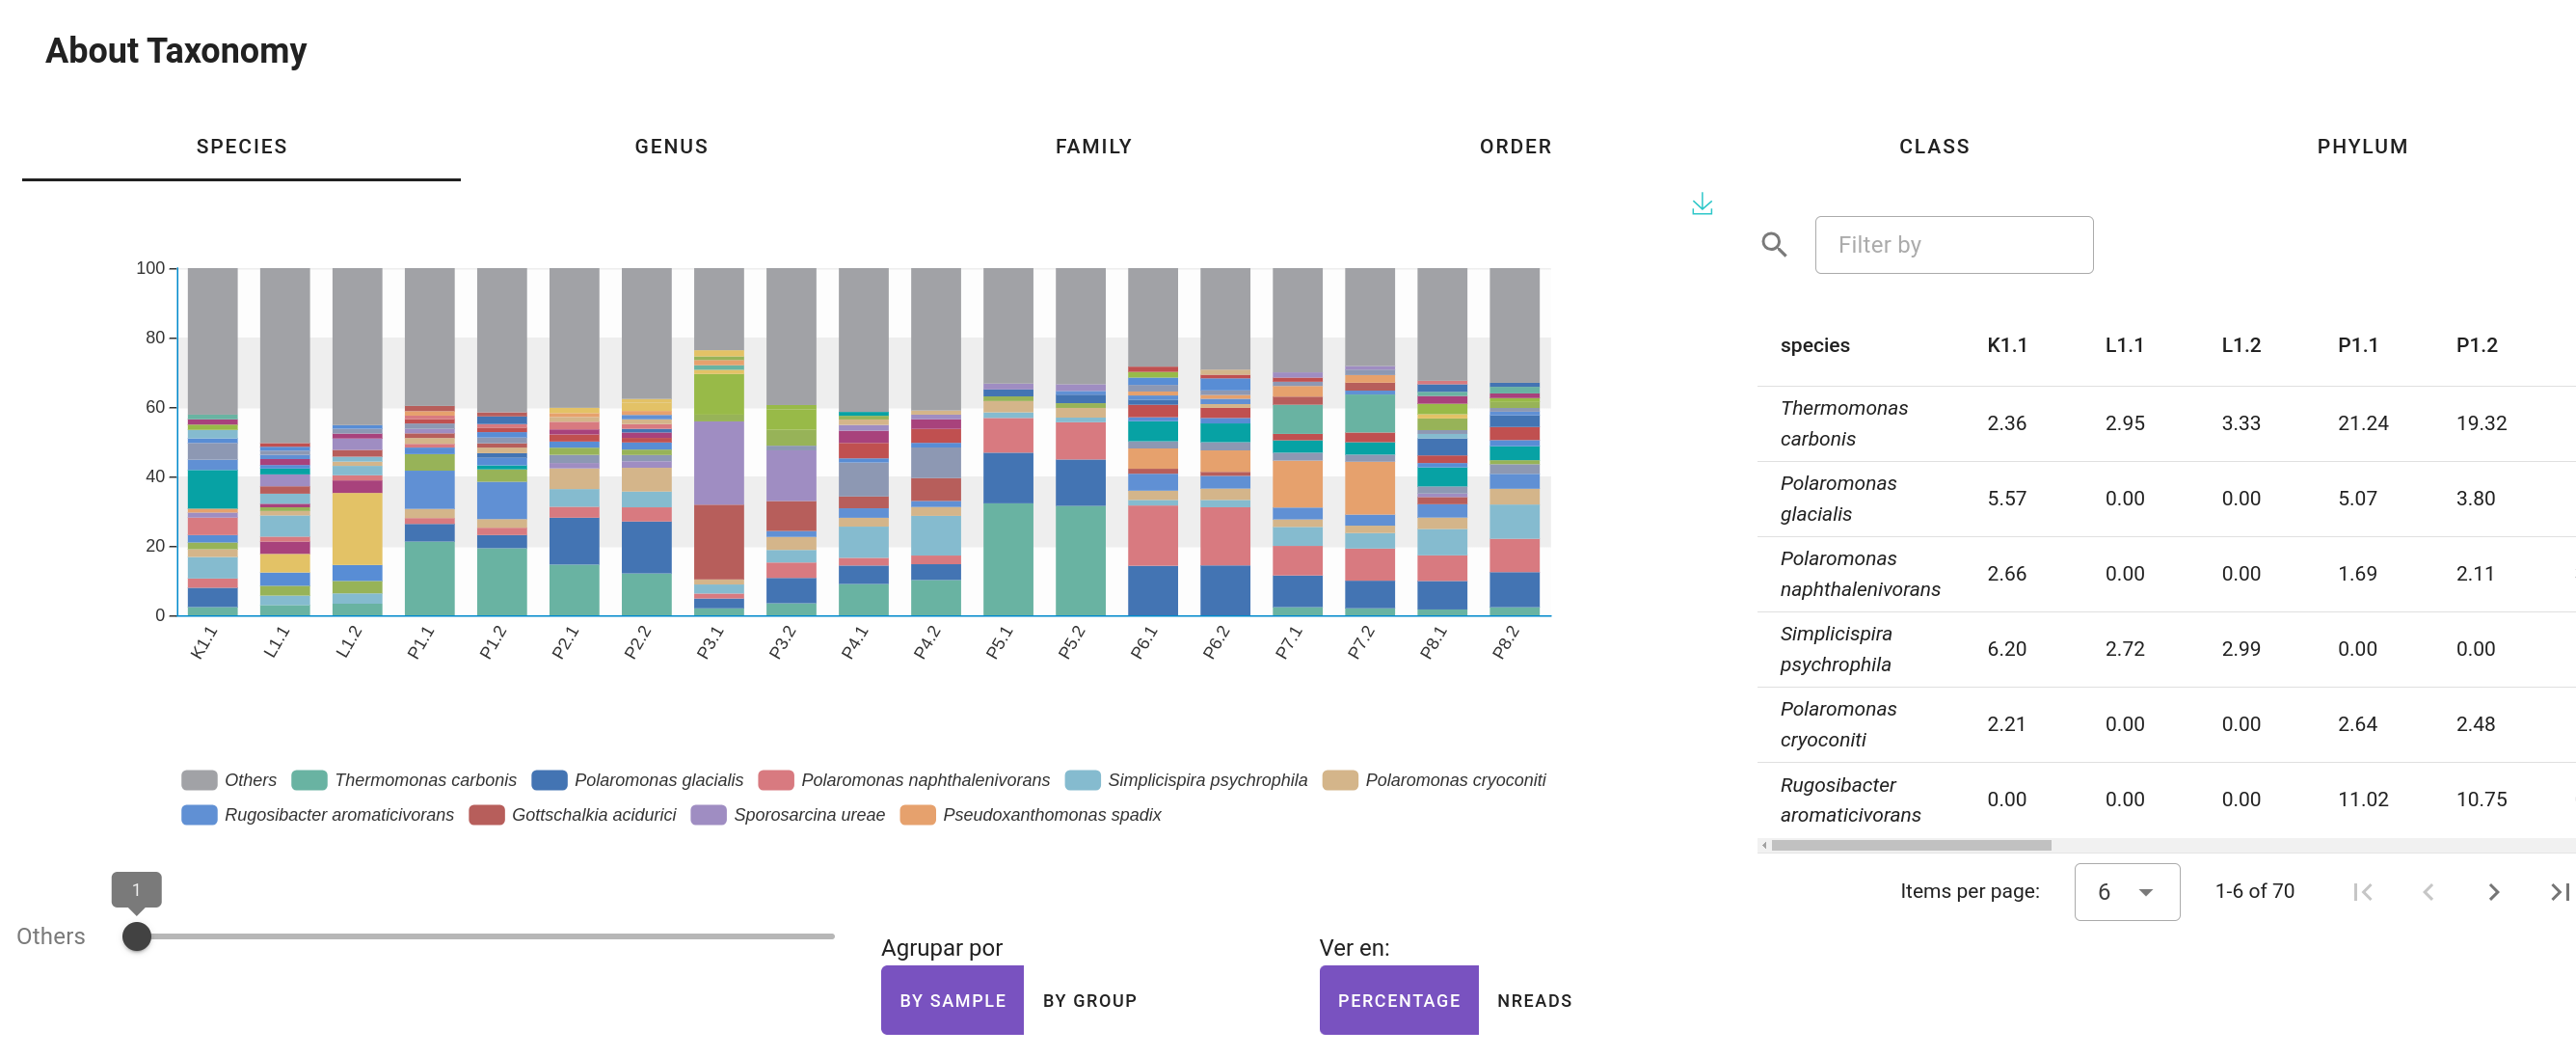
\includegraphics[width=1\linewidth]{images/app/results/taxonomy.png}
    % \captionsetup{justification=raggedright, width=0.45\linewidth, singlelinecheck=off}

    % \captionsetup{width=0.45\linewidth}
    \caption{Vista de asignación taxonómica (resultados)}
    \label{fig:app-results-taxonomy}
\end{figure}

% En el lado derecho, hay una tabla que permite visualizar el detalle de la información presentada en el gráfico. 
% Se puede visualizar además un campo de texto que permite al usuario buscar una taxonomía en especifico y visualizar su abundancia o cantidad de lecturas en todas las muestras.

En caso de que la pantalla tenga una resolución menor a \hl{XX} la tabla y gráfico se desplegarán uno debajo del otro(Figura~\ref{fig:app-results-taxonomy-small-dev}).
\begin{figure}[H]
    \centering
    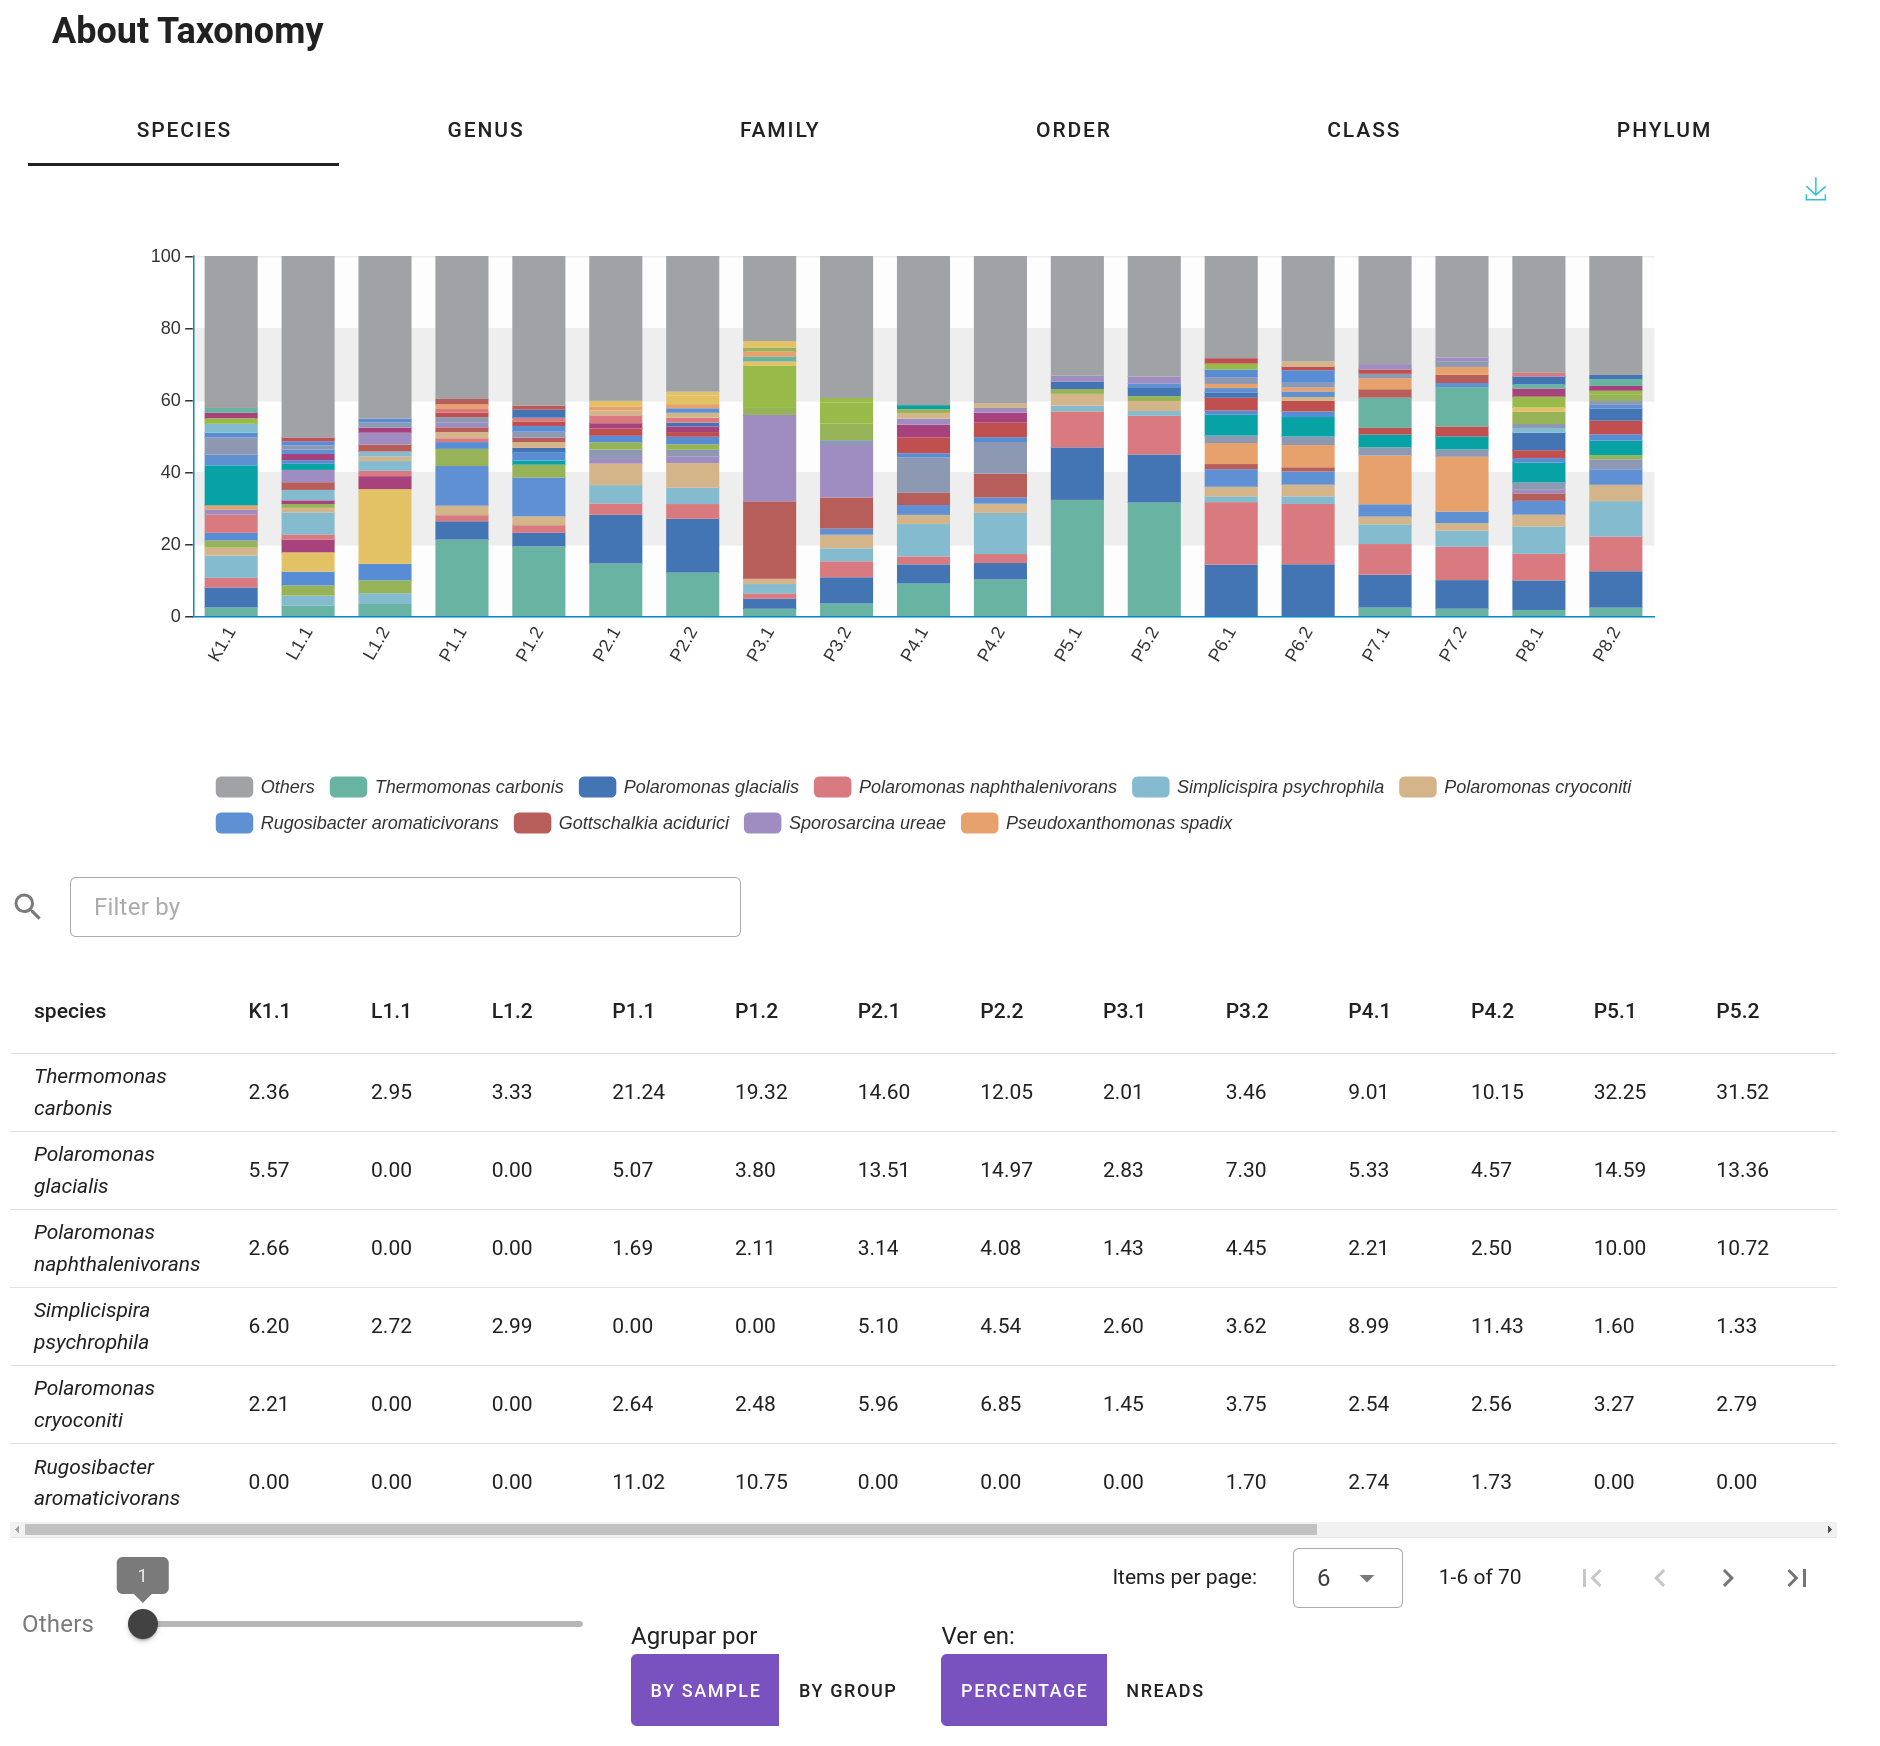
\includegraphics[width=0.8\linewidth]{images/app/results/taxonomy_small_dev.png}
    % \captionsetup{justification=raggedright, width=0.45\linewidth, singlelinecheck=off}

    % \captionsetup{width=0.45\linewidth}
    \caption{Estadisticas básicas (resultados)}
    \label{fig:app-results-taxonomy-small-dev}
\end{figure}

Ambos componentes, la tabla y el gráfico de barras apiladas se ajustan automáticamente para presentar la información requerida por el usuario, es decir, cada vez que el usuario selecciona una nueva categoría taxonómica en las pestañas, se vuelve a generar la información proporcionando una visualización clara y detallada de los datos.







% El usuario puede modificar la visualización de la información en el gráfico de barras apiladas y tabla a través de las pestañas que se encuentran en la parte superior del gráfico 
En la Figura~\ref{fig:app-results-taxonomy-order} el usuario seleccionó la pestaña de orden, por lo que se visualiza la información de la taxonomía en la categoría de orden.
\begin{figure}[H]
    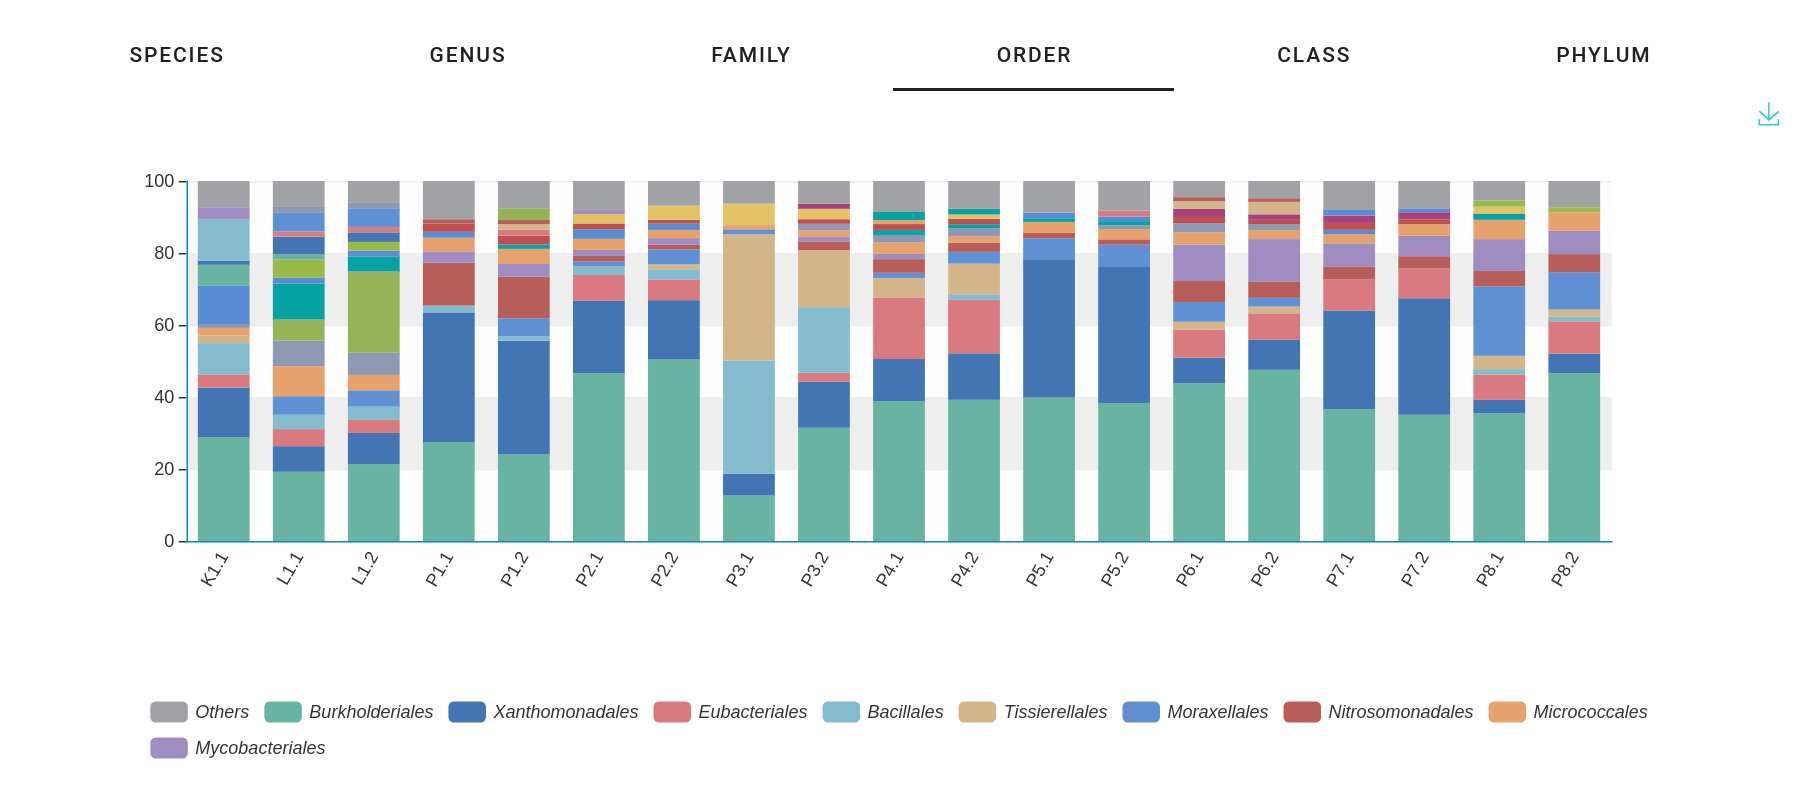
\includegraphics[width=1\linewidth]{images/app/results/taxonomy_order.png}
    % \captionsetup{justification=raggedright, width=0.45\linewidth, singlelinecheck=off}

    % \captionsetup{width=0.45\linewidth}
    \caption{Vista de asignación taxonómica en categoría de orden (stacked plot)}
    \label{fig:app-results-taxonomy-order}
\end{figure}



% \begin{figure}[H]
%     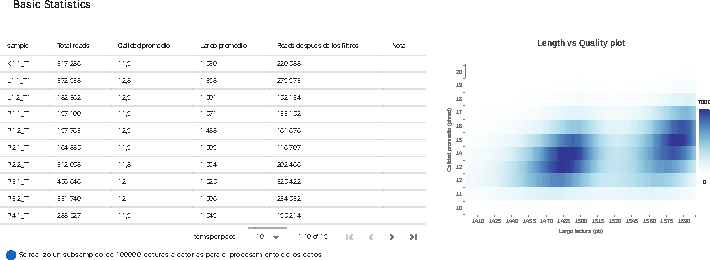
\includegraphics[width=1\linewidth]{images/app/results/basicStatistics.png}
%     % \captionsetup{justification=raggedright, width=0.45\linewidth, singlelinecheck=off}

%     % \captionsetup{width=0.45\linewidth}
%     \caption{Estadisticas básicas (resultados)}
%     \label{fig:app-results-taxonomicAssig-group-perc}
% \end{figure}




El usuario también puede modificar la información de la tabla y gráfico utilizando los botones que se encuentran en la parte inferior del gráfico. 
Pudiendo visualizar la información en porcentaje o en cantidad de lecturas~\ref{fig:app-results-taxonomy-sample-nreads}, como también pudiendo agrupar las muestras por grupo~\ref{fig:app-results-taxonomy-groups-perc}.
\begin{figure}[H]
    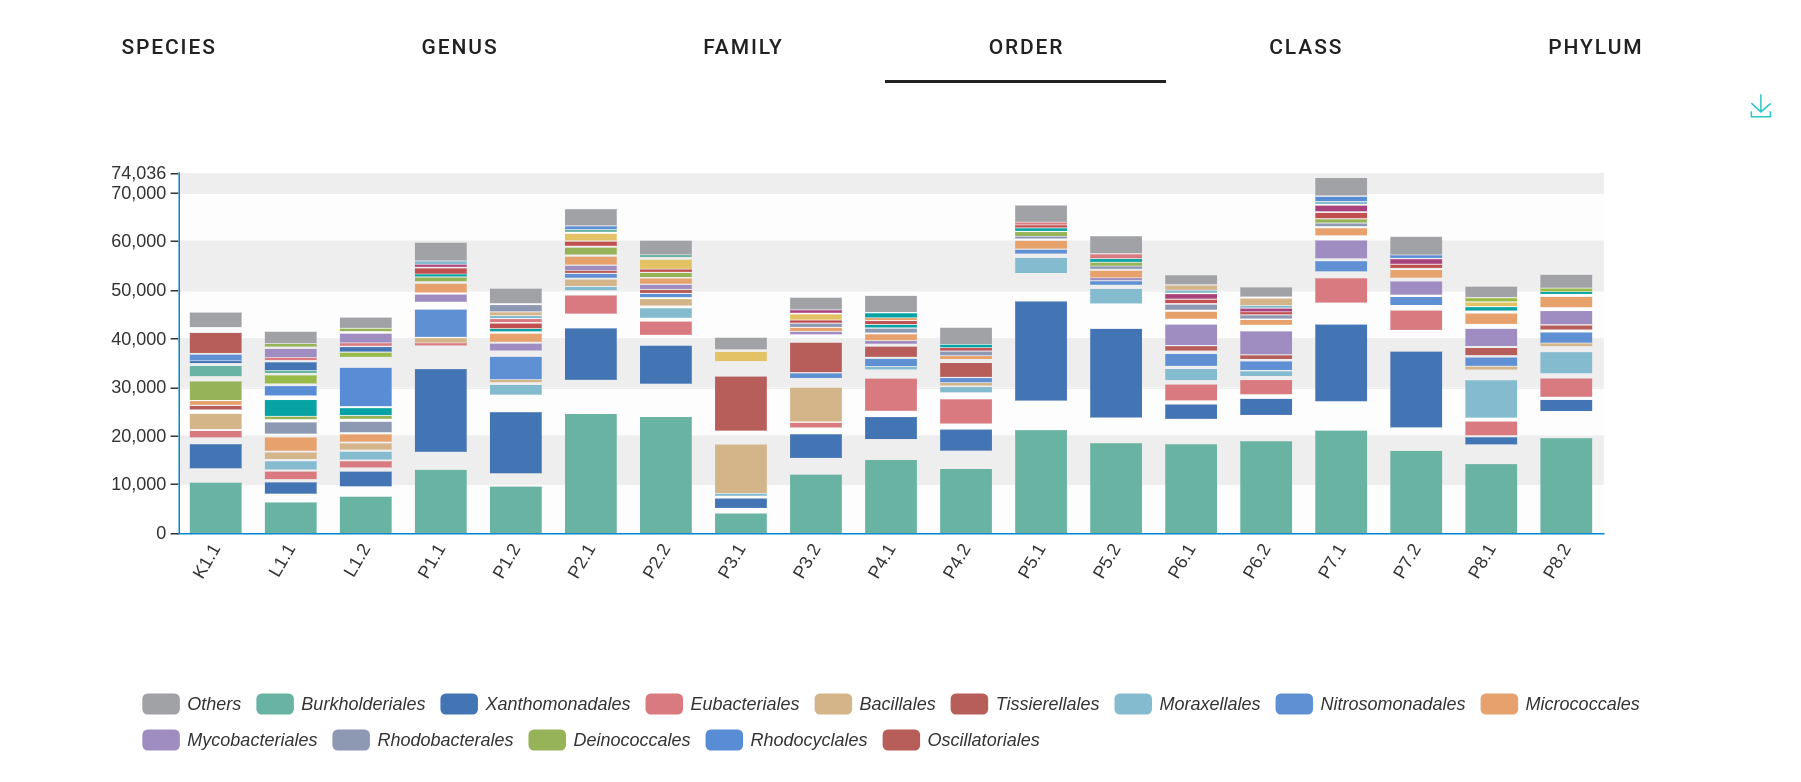
\includegraphics[width=1\linewidth]{images/app/results/taxonomy_sample_nreads.png}
    % \captionsetup{justification=raggedright, width=0.45\linewidth, singlelinecheck=off}

    % \captionsetup{width=0.45\linewidth}
    \caption{Taxonomias por muestra utilizando cantidad de lecturas}
    \label{fig:app-results-taxonomy-sample-nreads}
\end{figure}

\begin{figure}[H]
    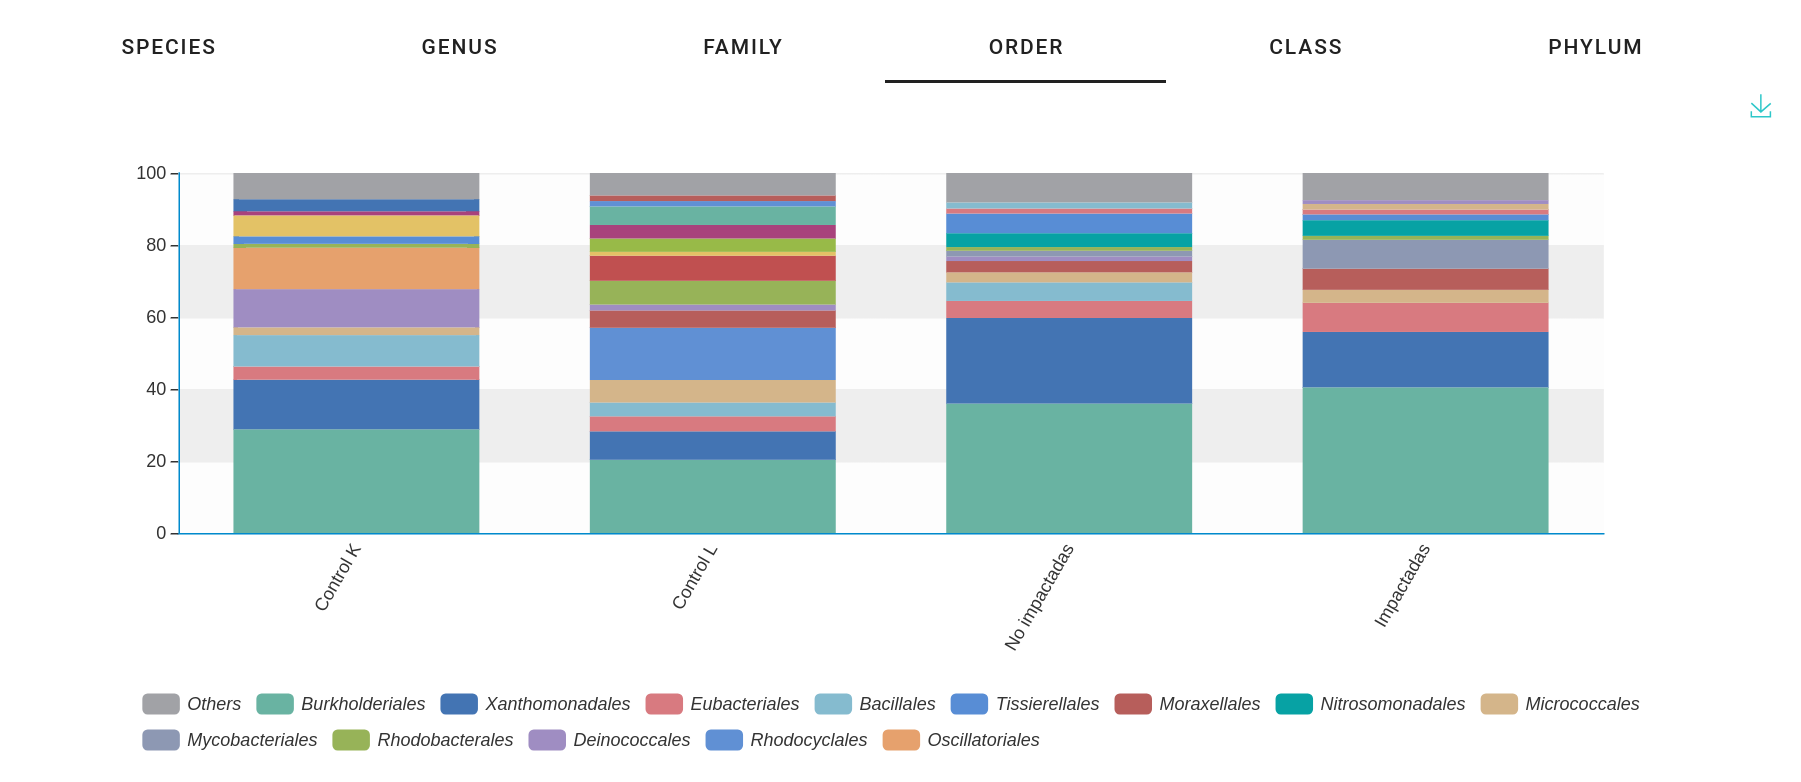
\includegraphics[width=1\linewidth]{images/app/results/taxonomy_grooups_perc.png}
    % \captionsetup{justification=raggedright, width=0.45\linewidth, singlelinecheck=off}

    % \captionsetup{width=0.45\linewidth}
    \caption{Taxonomias por grupo utilizando valor porcentual}
    \label{fig:app-results-taxonomy-groups-perc}
\end{figure}


De igual forma el usuario puede posicionar el mouse sobre alguna barra del gráfico o sobre alguna taxonomía de la leyenda y destacar esa taxonomía en todas las muestras y visualizar el porcentaje o cantidad de lecturas en la muestra que el mouse se encuentra posicionado (Figura~\ref{fig:app-results-taxonomicAssig-others}).
\begin{figure}[H]
    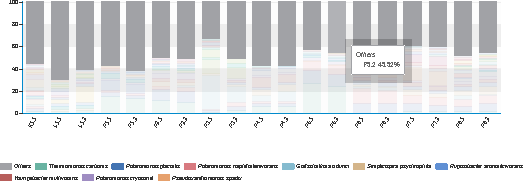
\includegraphics[width=1\linewidth]{images/app/results/taxonomy_others.pdf}
    % \captionsetup{justification=raggedright, width=0.45\linewidth, singlelinecheck=off}

    % \captionsetup{width=0.45\linewidth}
    \caption{Taxonomía por muestra: Destacar taxonomía en todas las muestras}
    \label{fig:app-results-taxonomicAssig-others}
\end{figure}


La tabla de taxonomías presenta un campo de búsqueda en la parte superior que permite al usuario filtrar la tabla por una taxonomía en especifico (Figura~\ref{fig:app-results-taxonomy-search}).
En el ejemplo se busca la palabra \textit{Polar} por lo que aparecen todas taxonomías que contienen esta palabra en su nombre.
\begin{figure}[H]
    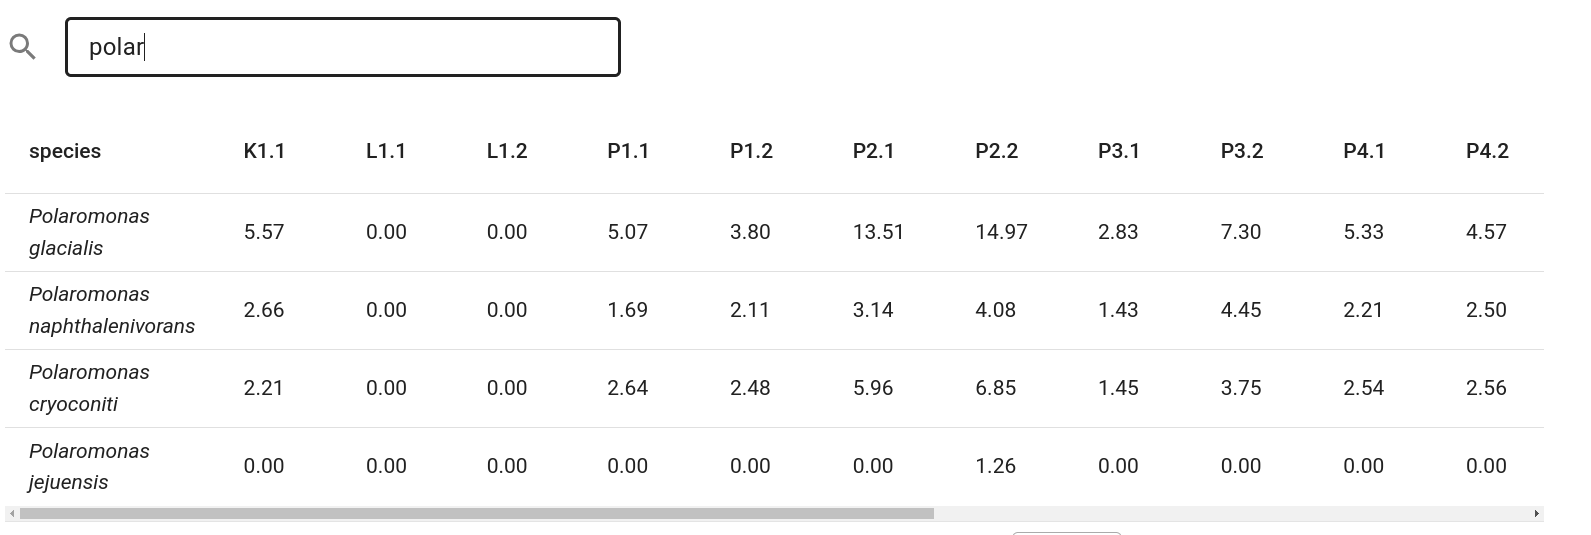
\includegraphics[width=0.9\linewidth]{images/app/results/taxonomy_search.png}
    % \captionsetup{justification=raggedright, width=0.45\linewidth, singlelinecheck=off}

    % \captionsetup{width=0.45\linewidth}
    \caption{Filtro de resultados en tabla de asignación taxonómica}
    \label{fig:app-results-taxonomy-search}
\end{figure}

\subsection{Similitud entre las muestras}
Esta sección representa las taxonomías compartidas por las muestras mediante un gráfico circular de anillos jerarquicos. 
Cada nivel del gráfico representa una categoría taxonómica, siendo la más interna especie, y la más externa filo.
Mientras más grande el diamentro del anillo en el gráfico, mayor es la presencia de esa taxonomía en las muestras.

Las taxonomías presentadas incluyen todas las taxonomías con abundancia mayor al 1\% y que estan presentes en todas las muestras del grupo.
El porcentaje presentado corresponde el porcentaje de todas las lecturas en el grupo graficado.


A continuación se presenta un ejemplo de como se visualiza el gráfico circular de anillos jerarquicos para dos grupos(Figura~\ref{fig:app-results-core}).
\begin{figure}[H]
    \centering
    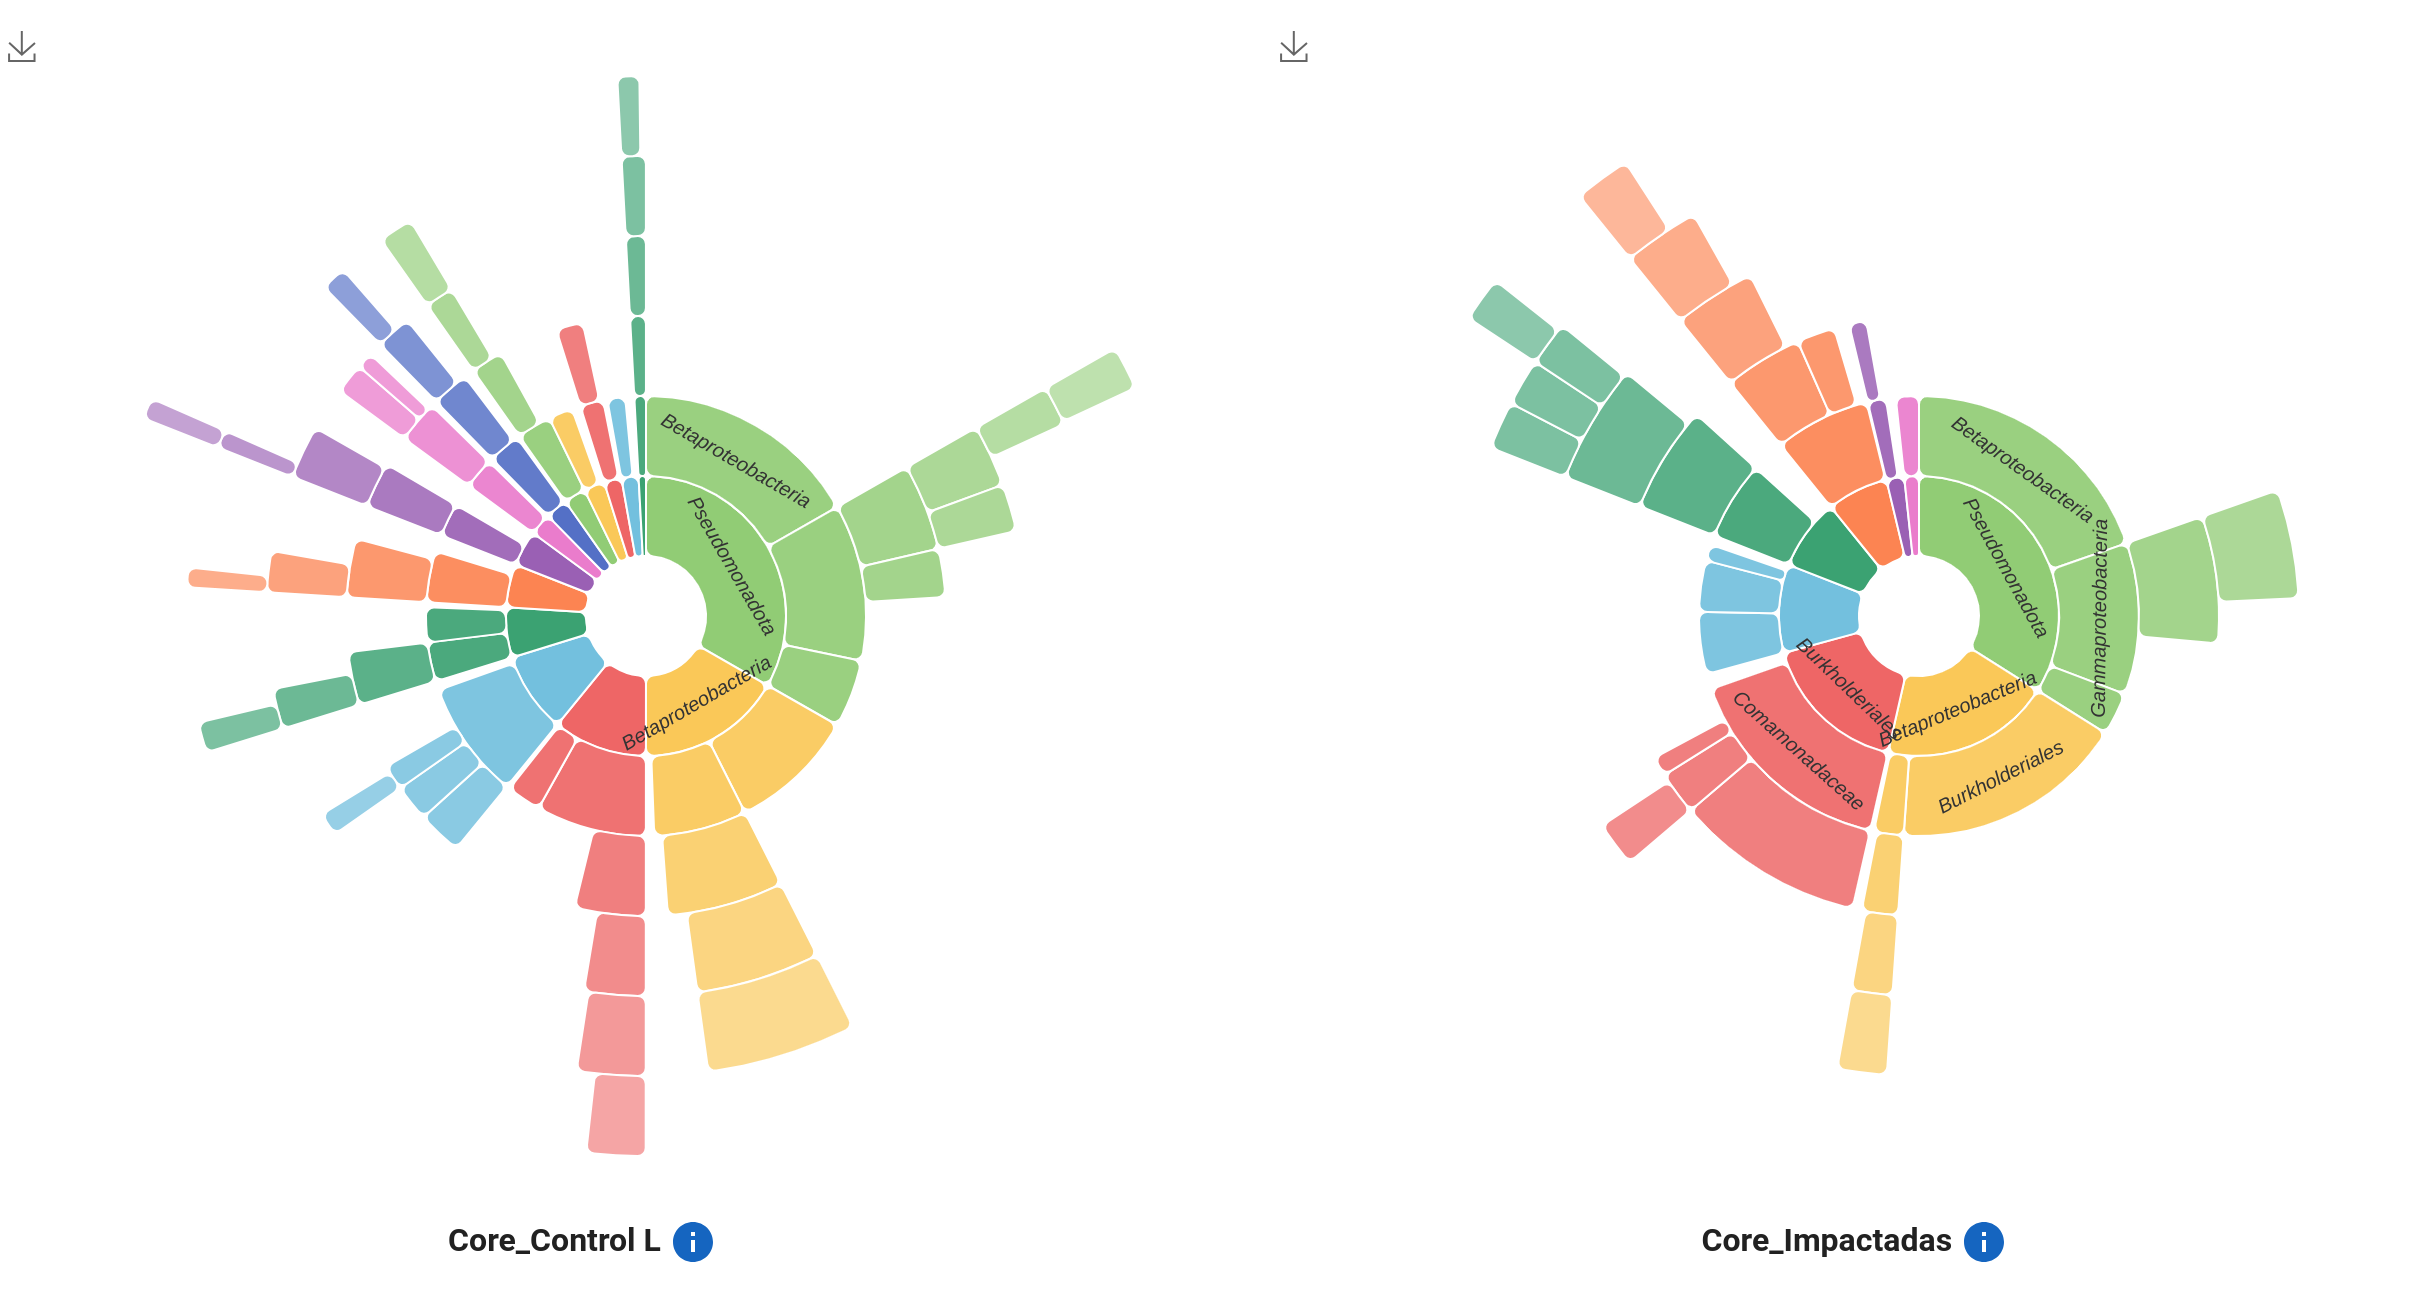
\includegraphics[width=0.8\linewidth]{images/app/results/core.png}
    % \captionsetup{justification=raggedright, width=0.45\linewidth, singlelinecheck=off}

    % \captionsetup{width=0.45\linewidth}
    \caption{Gráfico de similitud  (resultados)}
    \label{fig:app-results-core}
\end{figure}

En esta sección se puede presentar un solo gráfico de las taxonomías compartidas entre todas las muestras, y en el caso de que el usuario haya ingresado grupos, se desplegaran además los gráficos por cada grupo, como se visualiza en la Figura~\ref{fig:app-results-core}.

En la parte inferior del gráfico, al lado derecho de la leyenda se puede visualizar un icono, el cual al posicionarse sobre el, va a mostrar las muestras utilizadas para generar el gráfico(Figura~\ref{fig:app-results-core-tooltip}).

\begin{figure}[H]
    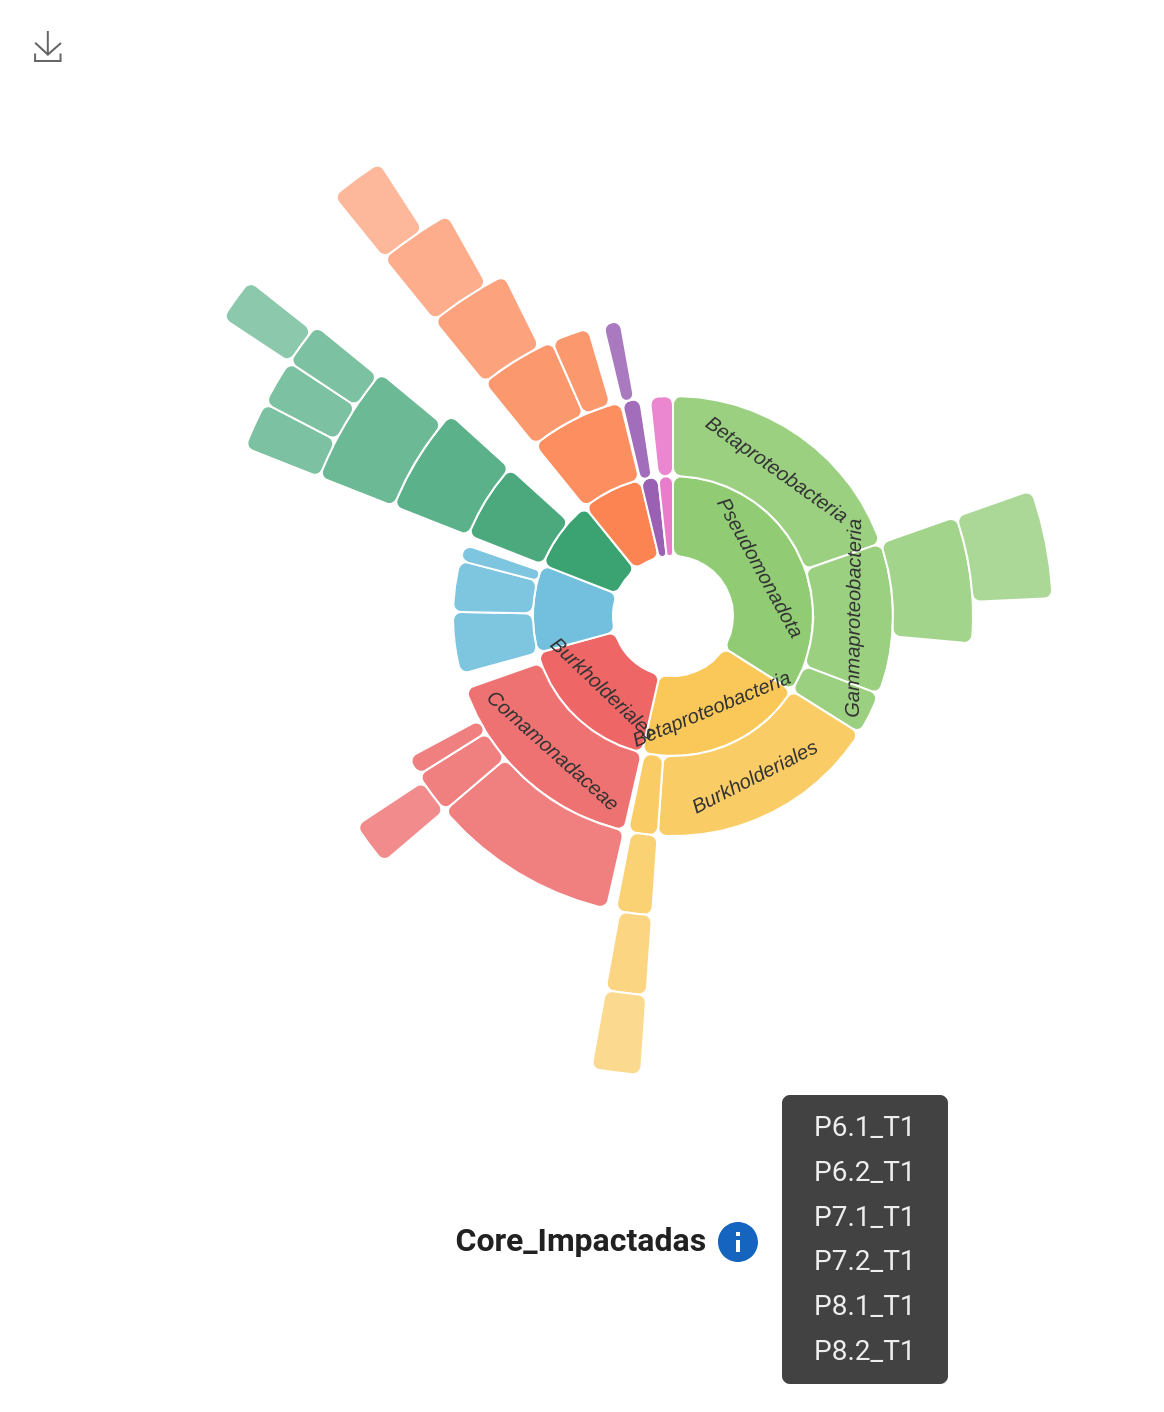
\includegraphics[width=0.8\linewidth]{images/app/results/core_tooltip.png}
    % \captionsetup{justification=raggedright, width=0.45\linewidth, singlelinecheck=off}

    % \captionsetup{width=0.45\linewidth}
    \caption{Gráfico de similitud: Tooltip asociado a las muestras (resultados)}
    \label{fig:app-results-core-tooltip}
\end{figure}

\subsection{Indices de diversidad}

En caso de que el usuario hubiera ingresado grupos al inicio del proyecto y hubiera activado los análisis de índices de diversidad, se podrá visualizar tres gráficos boxplot, uno por cada índice de diversidad (Shannon, Simpson y Chao2). En caso de que el usuario no haya ingresado grupos, esta sección no se desplegará en la plataforma.

A continuación se presenta un ejemplo de la visualización de esta sección en la plataforma:



\subsection{Predicción funcional}
Al igual que en la sección de asignación taxonómica, en la parte superior se pueden visualizar tres pestañas \textit{EC, KO y Pathways} que representan cada categoría funcional. Por defecto se presenta la información para la categoría de \textit{Pathways}.

En la parte inferior izquierda se puede visualizar una tabla con la información de la predicción funcional obtenida mediante PICRUSt2 (EC, KO y Pathways) para cada muestra. 
En la parte superior de la tabla se puede visualizar un campo de texto de búsqueda con el cual el usuario puede filtrar la información de la tabla.

En el lado derecho de la sección, en caso de que el usuario hubiera ingresado grupos, se puede ver un gráfico de barras horizontales que muestra los pathways con diferencias significativas entre los grupos (información obtenida mediante LEfSe). 
En caso de que no se haya ingresado información de grupos, solo se desplegará la tabla.

Al igual que en la sección de asignación taxonómica el usuario puede interactuar con las pestañas modificando el contenido de las tablas mediante la selección de las pestañas.


\begin{figure}[H]
    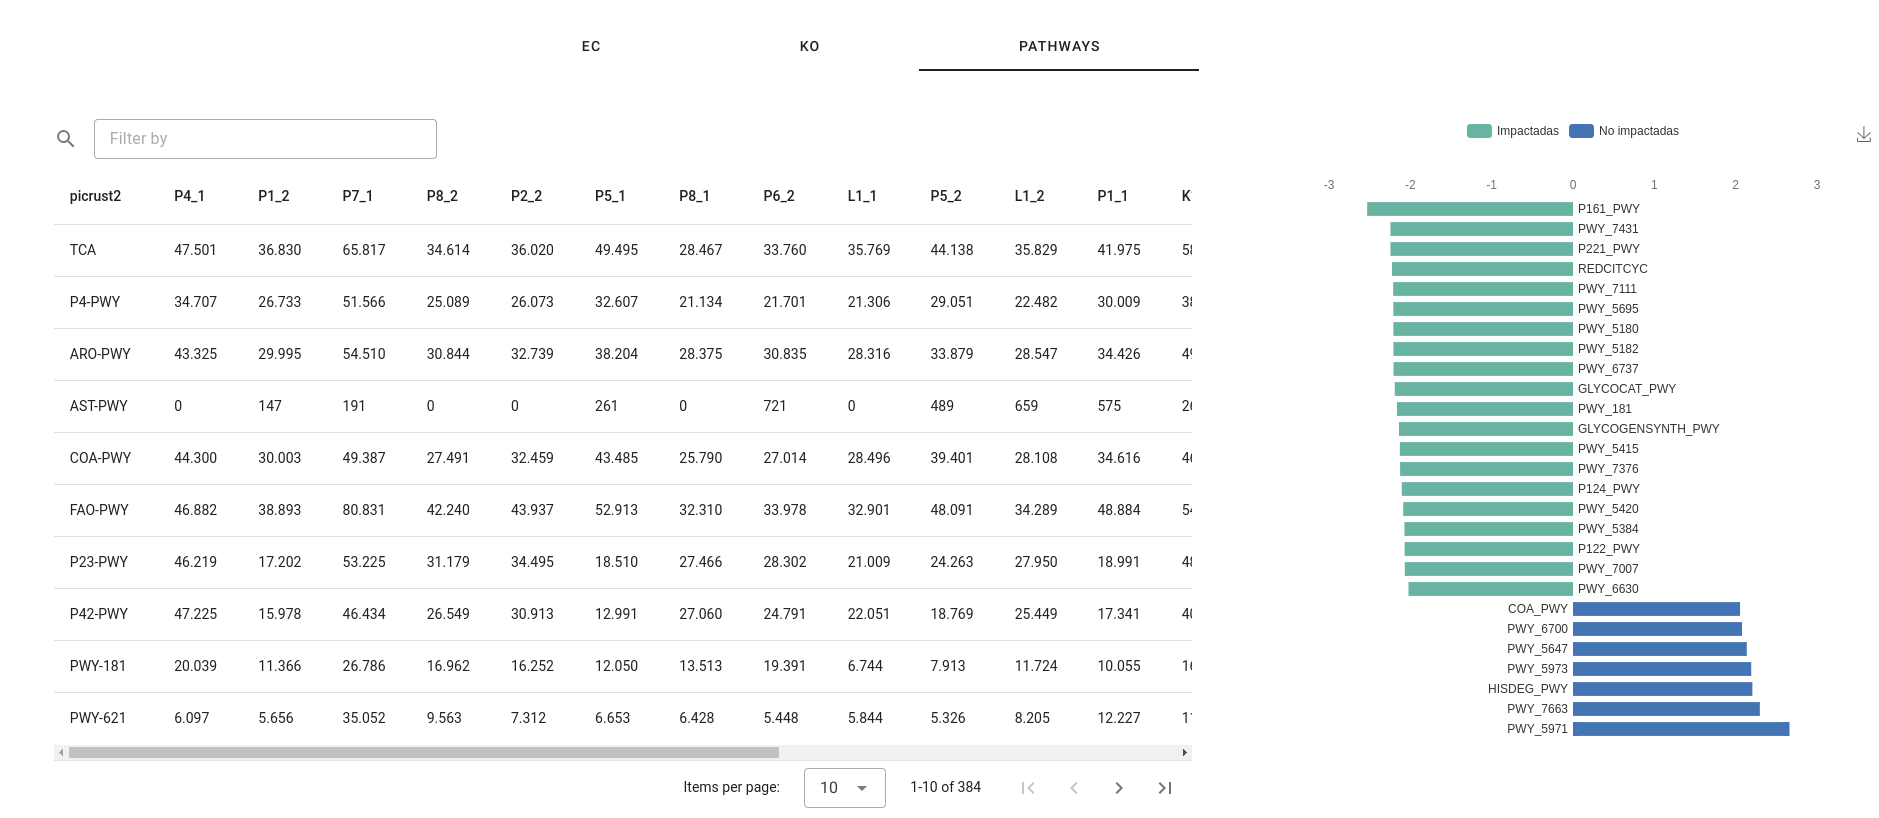
\includegraphics[width=1\linewidth]{images/app/results/functinoal_pred.png}
    % \captionsetup{justification=raggedright, width=0.45\linewidth, singlelinecheck=off}

    % \captionsetup{width=0.45\linewidth}
    \caption{Resultados de predicción funcional: Tabla obtenida mediante PICRUSt2 y gráficod de diferencias significativas obtenido mediante LefSE}
    \label{fig:app-results-functional-pred}
\end{figure}
\subsubsection{Descarga de los resultados}
En la parte superior derecha de la sección de resultados, se encuentra un botón con el texto \textit{Download data}. 
Al hacer click en este botón se descargará un archivo comprimido con toda los resultados generados por el pipeline.
A continuación se detallan los archivos:
\begin{itemize}
    \item CSV de asignación taxonomica por muestra y por grupo (en caso de ingresarse), y por porcentaje y cantidad de lecturas
    \item CSV de predicción funcional (EC, KO y pathways), en caso de haber seleccionado predicción funcional dentro de los análisis.
    \item CSV con los valores del cálculo de los indices de diversidad
    % \item \hl{PDF con los gráficos de barras apiladas, Sunburst y boxplot}
    % \item \hl{Archivo de texto con la información del pipeline (versión, parámetros, etc)}
\end{itemize}


\begin{figure}[H]
    
\includegraphics[width=1\linewidth]{images/app/donwload_button.png}
    % \captionsetup{justification=raggedright, width=0.45\linewidth, singlelinecheck=off}

    % \captionsetup{width=0.45\linewidth}
    \caption{Gráfico de similitud: Tooltip asociado a las muestras (resultados)}
    \label{fig:app-download-button}
\end{figure}

% \begin{figure}[H]
%     \includegraphics[width=1\linewidth]{images/app/results/downloadbutton.png}
%     % \captionsetup{justification=raggedright, width=0.45\linewidth, singlelinecheck=off}

%     % \captionsetup{width=0.45\linewidth}
%     \caption{Botón de descarga de resultados(resultados)}
%     \label{fig:app-results-download}
% \end{figure}

\subsection{Integración del flujo de trabajo y aplicación web}

Se diseñó una base de datos no relacional utilizando PostgreSQL.
Esta base de datos permite almacenar la información de los proyectos subidos por el usuario en la plataforma web y los resultados obtenidos al ejecutar el flujo de trabajo.
La base de datos funciona como intermedio entre el flujo de trabajo y la base de datos, permitiendo que la aplicación web escriba la metadata asociada al proyecto para que el flujo de trabajo pueda ejecutarse, y permitiendo además que la aplicación web pueda leer los resultados escritos por el flujo de trabajo, para poder convertir esta información en tablas y gráficos que permitan al usuario visualizar los resultados de manera sencilla.

La base de datos esta compuesta por siete tablas:
\begin{itemize}
    \item PlatformRoles: Almacena los roles de la plataforma (admin, basic user).
    \item Users: Almacena la información de los usuarios registrados en la plataforma.
    \item Projects: Almacena la información de los proyectos subidos por los usuarios.
    \item ProjectRoles: Almacena los roles de los usuarios dentro de los proyectos. Esto permite que un projecto y sus resultados puedan ser visualizados por varios usuarios a la vez.
    \item ProjectRolesUsers: Almacena la relación entre los usuarios y los roles de los proyectos. Permitiendo a los usuarios tener diferentes roles en diferentes proyectos (solo lectura, edición, eliminar).
    \item Results: Almacena los resultados obtenidos en la ejecución del flujo de trabajo.
    \item PipelineDefaultParams: Almacena los parámetros por defecto de cada versión del flujo de trabajo.
\end{itemize}

\begin{figure}[H]
    \centering
    \includegraphics[width=1\linewidth]{images/dbb.png}
    \caption{Base de datos}
    \label{fig:nanotax-db}
\end{figure}

Las tablas de Resultados y Proyectos estan compuestas por campos JSONB que permiten almacenar datos en formato JSON mediante una representación binaria permitiendo que los datos sean indexados y consultados de manera eficiente. 

Para la ejecución del flujo de trabajo se desarrollo un script en Python que escribe el archivo \textit{params.yml} con la información del proyecto y los parámetros ingresados por el usuario en la plataforma (y guardados en la base de datos).
Una vez que el pipeline finaliza su ejecucción mediante un script en Python se almacenan los resultados en la base de datos.

% \subsection{Documentación}
% En esta sección se despliega la documentación del pipeline, la cual cuenta con la información de los módulos, parámetros y herramientas utilizadas en el pipeline. La documentación se encuentra dividida por cada módulo, donde se muestra la versión de la herramienta utilizada y los parámetros por defecto y modificables por el usuario.
% \subsubsection{Basecalling y demultiplexación}
% \subsubsection{Control de calidad}
% \subsubsection{Asignación taxonómica}
% \subsubsection{Predicción funcional}
% \subsubsection{Indices de diversidad}


\chapter{Discusión}

La profundización en el estudio de la inteligencia artificial (\acrshort{ia}) nos conduce a un examen detallado de su impacto en múltiples facetas de la vida humana y la sociedad. Este campo, caracterizado por su dinamismo y potencial para la innovación, plantea tanto oportunidades como desafíos que merecen ser analizados con un enfoque crítico y constructivo.

\section{Impacto Social y Ético de la IA}

La inteligencia artificial (\acrshort{ia}) representa uno de los avances tecnológicos más significativos de nuestra era, ofreciendo un potencial extraordinario para el progreso humano pero también presentando desafíos éticos y sociales sin precedentes \cite{Smith2021}. A medida que integramos la \acrshort{ia} en diversos aspectos de la vida diaria, desde la asistencia sanitaria y la educación hasta la seguridad y el entretenimiento, es crucial reflexionar sobre su impacto en la sociedad y en los valores éticos fundamentales.

\subsection{Beneficios de la \acrshort{ia}}

La \acrshort{ia} tiene el potencial de transformar industrias, mejorar la eficiencia y resolver problemas complejos que han desafiado a la humanidad durante décadas \cite{Johnson2019}. Por ejemplo, en el sector de la salud, los sistemas de \acrshort{ia} pueden analizar grandes conjuntos de datos para diagnosticar enfermedades con mayor precisión y rapidez que los métodos tradicionales \cite{Garcia2020}. Asimismo, la \acrshort{ia} contribuye a la sostenibilidad ambiental mediante la optimización del uso de recursos en la agricultura y la producción energética \cite{Lee2018}, y fomenta la inclusión social al mejorar el acceso a servicios educativos y financieros para comunidades desatendidas \cite{Kumar2021}.

\subsection{Desafíos Éticos}

A pesar de estos beneficios, la implementación de la \acrshort{ia} plantea preguntas éticas fundamentales relacionadas con la privacidad, la seguridad, la equidad y la toma de decisiones autónoma \cite{Martinez2022}. La recolección y análisis de datos personales por sistemas de \acrshort{ia} pueden vulnerar la privacidad individual y exacerbar la vigilancia masiva \cite{Nguyen2020}. Además, la dependencia de \glspl{algoritmo} para tomar decisiones críticas, como en la justicia penal o en la contratación laboral, puede perpetuar sesgos y discriminación si no se diseñan y gestionan con cuidado \cite{Robinson2021}.

\subsection{Equidad y Justicia Social}

La \acrshort{ia} también plantea desafíos significativos en términos de equidad y justicia social \cite{Hernandez2023}. Existe el riesgo de que los beneficios de la \acrshort{ia} se distribuyan de manera desigual, exacerbando las desigualdades existentes entre diferentes grupos sociales y regiones geográficas. Además, la automatización impulsada por la \acrshort{ia} puede llevar a la pérdida de empleos en ciertos sectores, planteando preguntas sobre el futuro del trabajo y la seguridad económica \cite{Fisher2019}.

\subsection{Desarrollo Sostenible}

Finalmente, el impacto de la \acrshort{ia} en el desarrollo sostenible merece una atención especial \cite{Owen2022}. Aunque la \acrshort{ia} puede contribuir significativamente a los Objetivos de Desarrollo Sostenible (ODS) de las Naciones Unidas, como la mejora de la salud y el bienestar, la educación de calidad y la acción por el clima, su desarrollo y aplicación deben guiarse por principios de sostenibilidad ambiental, social y económica para evitar efectos adversos no intencionados \cite{Santos2020}.

En conclusión, el impacto social y ético de la \acrshort{ia} es multifacético y complejo, requiriendo un enfoque equilibrado que fomente la innovación tecnológica mientras se asegura que su desarrollo y uso sean responsables, justos y beneficiosos para toda la sociedad \cite{Williams2021}.

\section{Desarrollo Responsable y Ética de la IA}

El desarrollo responsable de la inteligencia artificial (\acrshort{ia}) es fundamental para asegurar que la tecnología se implemente de manera que beneficie a la sociedad, respetando al mismo tiempo los derechos humanos y los principios éticos \cite{Thompson2022}. Este enfoque implica la colaboración multidisciplinaria entre tecnólogos, filósofos, sociólogos y legisladores para abordar los desafíos éticos, legales y sociales que presenta la \acrshort{ia}.

\subsection{Principios Éticos en la \acrshort{ia}}

La adopción de principios éticos universales en el desarrollo de la \acrshort{ia} es crucial para guiar las decisiones de diseño y uso de manera que promuevan el bienestar humano y eviten el daño. Estos principios incluyen la justicia, la equidad, la transparencia, la responsabilidad y el respeto a la privacidad \cite{Williams2022}. Por ejemplo, la transparencia en los \glspl{algoritmo} de \acrshort{ia} permite a los usuarios entender cómo se toman las decisiones que los afectan, mientras que la responsabilidad asegura que los desarrolladores y usuarios de la \acrshort{ia} sean conscientes de las consecuencias de su implementación.

\subsection{Participación Pública y Transparencia}

Una participación pública amplia en el desarrollo de la \acrshort{ia} es esencial para construir sistemas que reflejen los valores y necesidades de la sociedad \cite{Martinez2023}. Esto incluye involucrar a las comunidades afectadas en el proceso de diseño y decisión, asegurando que los sistemas de \acrshort{ia} sean accesibles y útiles para todos. La transparencia en los procesos de desarrollo y en los criterios de toma de decisiones de los sistemas de \acrshort{ia} también es fundamental para ganar la confianza del público y facilitar la rendición de cuentas.

\subsection{IA y Derechos Humanos}

La integración de consideraciones de derechos humanos en el desarrollo de la \acrshort{ia} es vital para evitar la discriminación y proteger las libertades fundamentales \cite{Robinson2023}. Esto significa diseñar sistemas de \acrshort{ia} que respeten la privacidad, promuevan la igualdad y estén libres de sesgos. Es crucial que los desarrolladores de \acrshort{ia} se comprometan con las normas internacionales de derechos humanos y trabajen en estrecha colaboración con expertos en derechos humanos para evaluar y mitigar los riesgos potenciales asociados con el uso de la \acrshort{ia}.

\subsection{Colaboración Internacional}

Dado el alcance global de la \acrshort{ia} y su potencial para trascender fronteras, la colaboración internacional es esencial para desarrollar normas y estándares éticos universales \cite{Kumar2024}. Esto incluye el intercambio de mejores prácticas, la armonización de regulaciones y el trabajo conjunto en iniciativas de investigación para abordar los desafíos éticos de la \acrshort{ia} de manera colectiva. La cooperación internacional puede facilitar un enfoque equilibrado que promueva la innovación y al mismo tiempo asegure que el desarrollo de la \acrshort{ia} sea responsable y ético.

Conclusión: El desarrollo responsable y ético de la \acrshort{ia} es un imperativo global que requiere un esfuerzo colectivo y multidisciplinario. Al adherirse a principios éticos universales y fomentar la participación pública, la transparencia y la colaboración internacional, podemos asegurar que la \acrshort{ia} se desarrolle de una manera que beneficie a toda la humanidad y proteja nuestros valores y derechos fundamentales \cite{Hernandez2024}.

\section{Conclusión y Reflexiones Futuras}

En resumen, este trabajo ha explorado diversas facetas del desarrollo y la implementación de la inteligencia artificial (\acrshort{ia}), destacando tanto su potencial transformador como los desafíos éticos y sociales inherentes. A través de la discusión sobre el impacto social y ético de la \acrshort{ia}, así como el enfoque en un desarrollo responsable y ético, hemos subrayado la importancia de guiar la evolución de la \acrshort{ia} de manera que beneficie a la sociedad en su conjunto, respetando los principios éticos universales \cite{Hernandez2024}.

La \acrshort{ia} tiene el potencial de revolucionar sectores como la salud, la educación, el transporte y la seguridad. Sin embargo, para que este potencial se realice de manera ética y responsable, es crucial una reflexión continua y una colaboración activa entre investigadores, desarrolladores, legisladores y la sociedad \cite{Williams2022}. El desarrollo de la \acrshort{ia} no debe ser únicamente una cuestión técnica; debe ser también un proceso informado por consideraciones éticas, sociales y legales, asegurando que las tecnologías emergentes fomenten la inclusión, la equidad y la justicia.

Mirando hacia el futuro, es esencial que la comunidad internacional continúe trabajando juntos para establecer y mantener estándares éticos en el desarrollo de la \acrshort{ia}. Esto incluye la creación de marcos regulatorios que no solo promuevan la innovación sino que también protejan los derechos humanos y fomenten una gobernanza ética de la tecnología \cite{Kumar2024}. Asimismo, la educación y la sensibilización sobre la ética de la \acrshort{ia} deben ser una prioridad, preparando a las futuras generaciones para participar activamente en el diálogo y la toma de decisiones relacionadas con la \acrshort{ia}.

Finalmente, mientras avanzamos hacia un futuro cada vez más influenciado por la \acrshort{ia}, es imperativo que sigamos cuestionando y reevaluando nuestros enfoques para garantizar que la tecnología sirva al bien común. La investigación futura deberá centrarse no solo en los avances tecnológicos sino también en el desarrollo de herramientas y metodologías para evaluar el impacto social de la \acrshort{ia}, asegurando que podamos navegar por los desafíos que surjan de manera efectiva y ética \cite{Robinson2023}.

\textit{“La inteligencia artificial tiene el potencial de ser una de las fuerzas más beneficiosas en nuestra sociedad, pero solo si la comunidad global se une para garantizar que su desarrollo sea ético y en beneficio de todos. El futuro de la \acrshort{ia} es un lienzo en el que todos tenemos un papel que desempeñar.”}



\backmatter

\begin{multicols}{2}[\printbibheading]
	\printbibliography[heading=none]
\end{multicols}

\clearpage

% imprimir glosario y acrónimos, en caso de que sea en inglés se puede quitar `toctitle` y `title` para que no aparezca en español
\printnoidxglossary[toctitle=Glosario]

\printnoidxglossary[type=\acronymtype, toctitle=Acrónimos y Abreviaturas, title=Acrónimos y Abreviaturas]

\end{document}